% --------------------------------------------
% \documentclass[twocolumn]{aastex6}
% \documentclass[apj]{emulateapj}
\documentclass[iop]{emulateapj} %iop
\usepackage{amsmath}


preamble.tex
\slugcomment{To be Submitted}

\makeatletter
\renewcommand\normalsize{\@setfontsize\normalsize\@xpt{12.5}}
% \renewcommand\normalsize{\@setfontsize\normalsize{10.56}{11.4}}      % 11.5, 12.5
\makeatother

\usepackage{xcolor}
\definecolor{apcolor}{HTML}{b3003b}
\definecolor{dlcolor}{HTML}{FF7F00}
\newcommand{\AP}[1]{({\bf \color{apcolor} AP: #1})}
\newcommand{\DL}[1]{({\bf \color{dlcolor} DL: #1})}

\citestyle{aa}
\shorttitle{Dynamical Properties of Molecular Cloud Complexes in $z$\ssim6 Prototypical Galaxy
}
\shortauthors{Leung et al.}

\begin{document}
\title{
Dynamical Properties of Molecular Cloud Complexes in a Redshift 6 Prototypical Galaxy at the Epoch of Reionization
}


\author{T. K. Daisy Leung\altaffilmark{1, 2}}
\author{Andrea Pallottini\altaffilmark{3, 4}}
\author{Andrea Ferrara\altaffilmark{4, 5}}
\author{Mordecai-Mark Mac Low\altaffilmark{2, 6, 7, 8}}

\altaffiltext{1}{Department of Astronomy, Space Sciences Building, Cornell University, Ithaca, NY 14853, USA}
\altaffiltext{2}{Center for Computational Astrophysics, Flatiron Institute, Simons Foundation, 162 Fifth Avenue, New York, NY 10010, USA}
\altaffiltext{3}{Centro Fermi, Museo Storico della Fisica e Centro Studi e Ricerche ``Enrico Fermi'', Piazza del Viminale 1, Roma, 00184, Italy}
\altaffiltext{4}{Scuola Normale Superiore, Piazza dei Cavalieri 7, I-56126 Pisa, Italy}
\altaffiltext{5}{Kavli Institute for the Physics and Mathematics of the Universe (IPMU), The University of Tokyo, 5-1-5 Kashiwanoha, Kashiwa 277-8583, Japan}
\altaffiltext{6}{Institut f{\"u}r Theoretische Astrophysik, Zentrum f{\"u}r Astronomie der Universit{\"a}t Heidelberg, 69120 Heidelberg, Germany}
\altaffiltext{7}{American Museum of Natural History, 79th St.~at Central Park West, New York, NY 10024, USA}
\altaffiltext{8}{Department of Physics, Disque Hall, Drexel University, Philadelphia, PA 19104, USA}
\email{tleung@astro.cornell.edu}



\begin{abstract}
We study the dynamical properties of molecular clouds complexes and their temporal evolution in a prototypical galaxy 
at the Epoch of Reionization (EoR) using state-of-the-art cosmological zoom-in simulation, 
which includes a chemical network to determine the formation of molecular
hydrogen, heating and cooling of the ISM by metals, and stellar feedback.
We use a clump finder algorithm and a set of H$_2$ volumetric densities ($n_{\rm cut}$) 
to identify molecular complexes (MC) and their sub-structures.
We extract properties such as mass, size, Mach number, velocity dispersion, gas surface density, and virial parameter for each MC.
We find that the MC of \flower are highly supersonic, with high velocity dispersions ($\sigma\approx$\,200\,\kms) comparable to 
those observed in gas-rich galaxies in the local universe and at the peak epoch of cosmic \SF. 
The mass scale of the MCs is of the order of $10^{6.5-9}$\,\Msun. The $\sim$200\,pc-scale MCs found with a low density threshold 
correspond to the arms of the disk of \flower which break down into smaller $\lesssim$100\,pc-scale MCs at higher density thresholds. 
The more massive and bigger MCs in \flower compared to the Milky Way 
likely result from the higher gas mass fraction, surface density, and velocity dispersion, 
which set the scale for fragmentation.
% consistent with what has been found previously in higher resolution isolated simulation (our zoom-in sim here allows us to examine 
% the influence on the dynamics of MCs due to continuous gas accretion from the surrounding IGM).
We compare the dynamics of MCs in \flower to those observed in the local Universe in the context of the Larson's relation.
The MCs of \flower are found to have higher $\sigma$ and $\Sigma$ systematically regardless of the $n_{\rm cut}$ adopted.
The velocity dispersion remains $\gtrsim$100\,\kms even when we increase the $n_{\rm cut}$ and even for the 
the molecular substructures, likely resulting from 
the strong supernova and stellar feedback \flower experienced over the multiple episodes of bursty \SF.
Virial analysis indicates that the MC/arms of the main disk of \flower are unbound, but the substructures have lower virial parameter. 
This is consistent with the notion that collapsing structures result from gravitational instability within globally stable structures, which are 
supported by turbulence and rotation on large scale.
We also find $\alpha_{\rm vir}$\ssim1 for the MCs in the satellite galaxies, which we interpret as a result of the weaker stellar feedback as they have
experienced less episodes of \SF compared to \flower (also supported by the lower stellar-to-gas mass ratio of the latter).
MCs in the satellites are therefore likely collapsing structures. This paints a picture, in which at the EoR, \SF continues 
as gas is being accreted from the IGM.
We find no temporal variations in the MC dynamics over the course of 700\,Myr traced in our simulation, at least in terms of the scaling relations examined. 
Our results are independent of the volume density threshold adopted, except for the slope of the cumulative 
mass distribution, which steepens as we increase $n_{\rm cut}$. 
High resolution imaging of the first galaxies with ALMA and the ngVLA 
will be useful to test our findings and the validity of our simulation to shed
light on \SF since the cosmic dark ages.
\end{abstract}
\keywords{methods: data analysis --
          galaxies: high-redshift --
          galaxies: ISM --
          galaxies: evolution --
          galaxies: formation --
          galaxies: starburst --
          stars: formation}


\def\figpath{./Fig}

%--------------------------------------------------------------------------
%                                Introduction
%--------------------------------------------------------------------------
\section{Introduction}    \label{sec:intro}

The growth of galaxies and their subsequent evolution are governed by the baryon cycle ---
galaxies accrete gas from the intergalactic medium (IGM) to fuel \SF (and feed their supermassive blackholes)
and subsequent feedback replenishes and enriches the circumgalactic medium with part of this material.
The general consensus is that the growth of \highz galaxies are triggered and supported by massive
gas inflows from mergers and/or the cosmic web at early cosmic time, when the IGM and galaxies themselves 
are more gas-rich in their star-forming molecular
gas contents compared to present-day galaxies.
% while at a given snapshot, the gas mass fraction maybe low (esp. at high-z when
% the gravitational potential is still increasing), but their gas reservoirs
% are continuously being replenished.
These massive gas inflows in turn trigger gravitational instability and lead
to the formation of gas structures that are typically more massive and denser than those
observed in nearby galaxies, with masses of $M_{\rm cloud}$\eq10$^9$\,\Msun
and sizes on sub-kpc scales (e.g., \citealt{Gabor13a, Hopkins14a, Inoue16a}).
Some theoretical works argue that the
migration of such giant massive clumps are responsible for contributing to the
buildup of the bulges of massive galaxies at \z$\sim$0 \citep[e.g.,][]{Ceverino10a}.

Given that \highz galaxies are the early stages of evolution of present-day galaxies, studying their ISM properties is essential for understanding how \SF proceed under these more extreme conditions, thereby driving the evolution and assembly history of galaxies 
since the cosmic dark ages.
Current consensus is that at higher redshifts, galaxies have higher 
star formation rates \citep[SFR; ][]{Behroozi13b, Sparre15a, Maiolino15a, Dunlop17a} and 
smaller sizes \citep[e.g.,][]{Bouwens11a, Ono13a} compared to those found in the local Universe.
The former are thus expected to have more \ion{H}{2} regions, ionized gas, and more intense radiation stellar feedbacks. 
Since their metallicity and dust content are also expected to be lower as they are assembling, 
this affects the shielding of UV photons, heating and cooling mechanisms in these early systems. Such differences in turn 
affect the regulation of thermal and chemical structures of their ISM. 
Their multi-phase ISM and the dynamics of the star-forming molecular cloud complexes (MC)
are therefore expected to differ from nearby galaxies.
Even in the local Universe, where the most detailed \obs can be attained, variations in cloud properties have been 
observed between different galaxy populations (see e.g., \citealt{Hughes10a, Hughes13b}).
It is thus obvious and reasonable to pose the question: what are the dynamical states of the MCs of the first galaxies and 
how do they differ from the local Universe, and are they analogous to any seen in the local \galpop?
% 

The FIR fine-structure lines (e.g., \cii, \nii, and \oiii), and CO/[\ci]~lines are the key diagnostics for
constraining the ISM conditions of galaxies and
provide highly complementary information tracing the different phases of the ISM (ionized,
atomic, molecular; e.g., \citealt{Scoville74a, Rubin85a, Malhotra01a}).
Global measurements of these diagnostics in \highz galaxies
have informed us on their galaxy-wide properties (e.g.,
gas masses, gas temperature, and radiation field intensity).
However, spatially resolving their ISM is needed in order to understand their role in galaxy evolution and
the physics behind their intense \SF (SFR\ssim100$-$3000\,\Msun\,yr\pmOne).
To date, spatially resolved ISM properties of \highz galaxies
have only been examine observationally in a handful of (strongly-lensed)
galaxies, using tracers such as
dust continuum, CO, and \cii lines (e.g., \citealt{Swinbank11a, Hodge15a, Ferkinhoff15a, Hodge16a},
Leung et al. 2018, submitted).
These studies find that galaxies at $z$\ssim2 galaxies, close to the peak of cosmic \SF, are more
molecular gas-rich, turbulent, and clumpy than nearby galaxies.
That said, it remains unclear how \SF proceed in the (sub-)$L^*$ galaxy population at \z$\gtrsim$\,6 --- 
at the epoch of reionization  ---
which is responsible for producing the
ionizing photons that reionized the Universe.

While ALMA has enabled the detections of
ISM diagnostic lines e.g., the \cii158\,$\micron$ and CO line emission in
normal (SFR$<$\,100\,\Msun\,yr\pmOne) galaxies at \z$>$\,6 over the past few years \citep[e.g.,][]{Smit18a},
we are still far from mapping their molecular ISM due to the cosmological dimming.
As such, we have undertaken a study, exploiting
state-of-the-art cosmological zoom-in hydrodynamic simulation
\ncode{Serra} (Greenhouse in Italian; \citealt{Pallottini17a, Pallottini17b}), to examine
the dynamical properties of the molecular cloud complexes in a \z$\sim$6 prototypical (i.e., $L^*$) 
galaxy.

This paper is structured as follows.
\AP{TBM}
In \Sec{sim}, we describe the setup of our simulation and the properties of our galaxy (\flower),
and describe the method used to identify its molecular gas complexes (MC).
In \Sec{results}, we present scaling relations based on
the MC identified and compare them with observations of molecular
(sub-)structures seen in nearby and \z$>$\,0 galaxies.
We present Toomre stability analysis in \Sec{Q} and
the cumulative mass distribution of the MCs in \flower in \Sec{cmf}.
In \Sec{diss}, we discuss the results and implications of our findings,
and present our conclusions in \Sec{conclusion}.
Throughout this paper, we adopt a concordance cosmology, with total matter, vacuum and baryonic densities
in units of the critical density $\Omega_{\Lambda}$\eq0.692, $\Omega_m$\eq0.308, $\Omega_b$\eq0.0481,
Hubble constant $H_0$\eq100\,$h$\,km s\pmOne\,Mpc\pmOne with $h$\eq0.678,
spectral index $n$\eq0.967 and $\sigma_8$\eq0.826 \citep{Planck14a}.


% ------------------
\section{Method: Simulation and ``Clump''-finding} \label{sec:sim}


\subsection{\ncode{Serra} Simulation\footnote{Serra means greenhouse in Italian which is motivated by the
fact that our simulation includes a chemical network to calculate the abundance of H$_2$, which in turn
dictates the formation of CO.
}}
The simulation used in this work is described by \citealt{Pallottini17a} and is briefly summarized here.

\ncode{Serra} is a cosmological zoom-in simulation performed using Eulerian hydrodynamics and
adaptive mesh refinement (AMR) technique to achieve high spatial resolution in the region of interest (i.e., regions of high baryonic density).
In particular, it uses a modified version of \ncode{ramses} \citep{Teyssier2002a} as the AMR backend.
%\ncode{Serra} uses sub-grid models that simultaneously account for the radiative transfer, clumpy structure, and photoevaporation feedback in the neutral diffuse and molecular gas.
Our simulation covers a co-moving box of 20\,Mpc $h$\pmOne in size, resolving down to a physical scale of 30\,pc (at \z$\sim$\,6) and a (baryonic) mass resolution of $m_b\simeq$\,10$^4$\,\Msun in the finest level. Such a physical scale is close to the size scale of molecular cloud complexes and giant molecular clouds (GMCs), as seen in nearby galaxies \citep[e.g.,][]{Sanders85a, Federrath13a, Goodman14a}.
% (Giant molecular clouds: L>22pc, m>10^5 Msun) in MW.
We include chemical network in the simulation to trace $\rm{H}$, $\rm{H}^{+}$, $\rm{H}^{-}$, $\rm{He}$, $\rm{He}^{+}$, $\rm{He}^{++}$, $\rm{H}_2$, $\rm{H}_2^{+}$ \citep{Grassi14a,Bovino16a}.
Of particular importance to our study here is that our simulation includes non-equilibrium formation of molecular hydrogen (done on-the-fly) to determine the H$_2$ abundance (see \citealt{Pallottini17b} for effects of chemistry affected by non-equilibrium versus equilibrium H$_2$ formation).

% radiative feedback --> NT pressure
Star formation is modeled using a H$_2$-based prescription of the Schmidt-Kennicutt relation \citep{Krumholz09a}. We adopt stellar tracks from \ncode{starburst99} and include stellar feedback from supernovae and OB/AGB stars to account for energy dissipations. To couple the feedback to the gas, we employ sub-grid modeling for blastwaves, e.g., to account for the potential lost of energy inside the cell when supernovae explode. The energy dissipated is then injected into the ISM in the form of kinetic and thermal energy. Radiation pressure on the dust and gas is also included (see \citealt{Pallottini17a} for details).

Details on the properties of \flower\ --- the main galaxy in our simulation --- are discussed in \citet{Pallottini17b}.
Briefly, by \z$\sim$6, \flower is a Lyman-break galaxy (LBG) hosted in a dark matter halo of mass $M_{\rm DM}\simeq$\,10$^{10}$\,\Msun at the center of a cosmic web knot, and accretes mass from the IGM mainly via three filaments of length $\simeq$\,100\,kpc. At \z$\sim$6, \flower has a stellar mass of $M_*\simeq$\,3\E{10}\,\Msun, a metallicity of $Z\simeq$\,0.5\,$Z_{\odot}$, a molecular gas mass of $M_{\rm H2}\simeq$\,5\E{7}\,\Msun, and a globally-integrated SFR of $\simeq$\,100\,\Msun\,yr\pmOne. It is therefore a prototypical galaxy at \z$\sim$6.

The simulation data contain information such as the density ($\rho$) and velocity ($v_x$, $v_y$, and $v_z$) fields, from which we calculate 
the physical properties of each MC, such as mass and velocity dispersion.
Due to the nature of our AMR simulation, we regrid the simulation data into uniform grids for the analysis presented in this paper. 
The grid size is defined 
based on the highest resolution of the simulation data (i.e., the less refined regions are supersampled in the resulting uniform grids). 



\subsection{Star Formation History} \label{sec:sfh}
One of the advantage of studying the dynamical properties of molecular structures at
$z$\ssim6 in simulation is the fact that we can examine how their properties evolve
as a function of time.
This is advantageous especially at early cosmic epochs,
when the densest structures are beginning to form;
gas is constantly being accreted onto the central galaxy from the cosmic web and
satellite galaxies, thereby leading to bursts of \SF.
Meanwhile, tidal forces resulting from interactions with these surrounding
galaxies can disrupt the main disk and arms, likely leading to different dynamical states
for the molecular structures compared to more evolved galaxies found at 
a later cosmic time (e.g., some molecular structures may disperse while others may agglomerate into more massive
ones). % mainly expecting differences in alpha_vir, sigma, M_cl.

We show the \SF history of \flower in \Fig{SFH}, where
the SFR of \flower varies between $\sim$30$-$80\,\Msun\,yr\pmOne\footnote{
The SFR plotted in Figure 2 of \citet{Pallottini17b}
is a factor of two higher than shown here since they also include contributions from
massive satellites galaxies within the surrounding $\approx$50\,kpc, which
are accreted onto \flower at \z$\lesssim$\,2.}
as it evolves from an actively accreting phase to
a starburst phase after a major merger, and then back to a relatively quiescent phase
over the few hundred Myr simulated in our simulation.
The SFR of \flower is calculated based on existing young stellar population, which is
defined to have an age of $t_{\rm age}<$\,10\,Myr.

Given the stochasticity in the \SF history of \flower,
we show the scaling relations found for two particular snapshots/evolutionary stages of \flower
as examples in \Sec{singless} to illustrate the salient points of the discussion,
since they represent the extreme evolutionary stages of \flower (and thus, likely bracket the
most extreme variations in the cloud dynamics) --- one of which \flower is
actively accreting materials from its surrounding 
and another of which \flower is undergoing
a starburst phase after a major merger (see \Fig{SFH}).

\begin{figure*}[htbp]
\centering
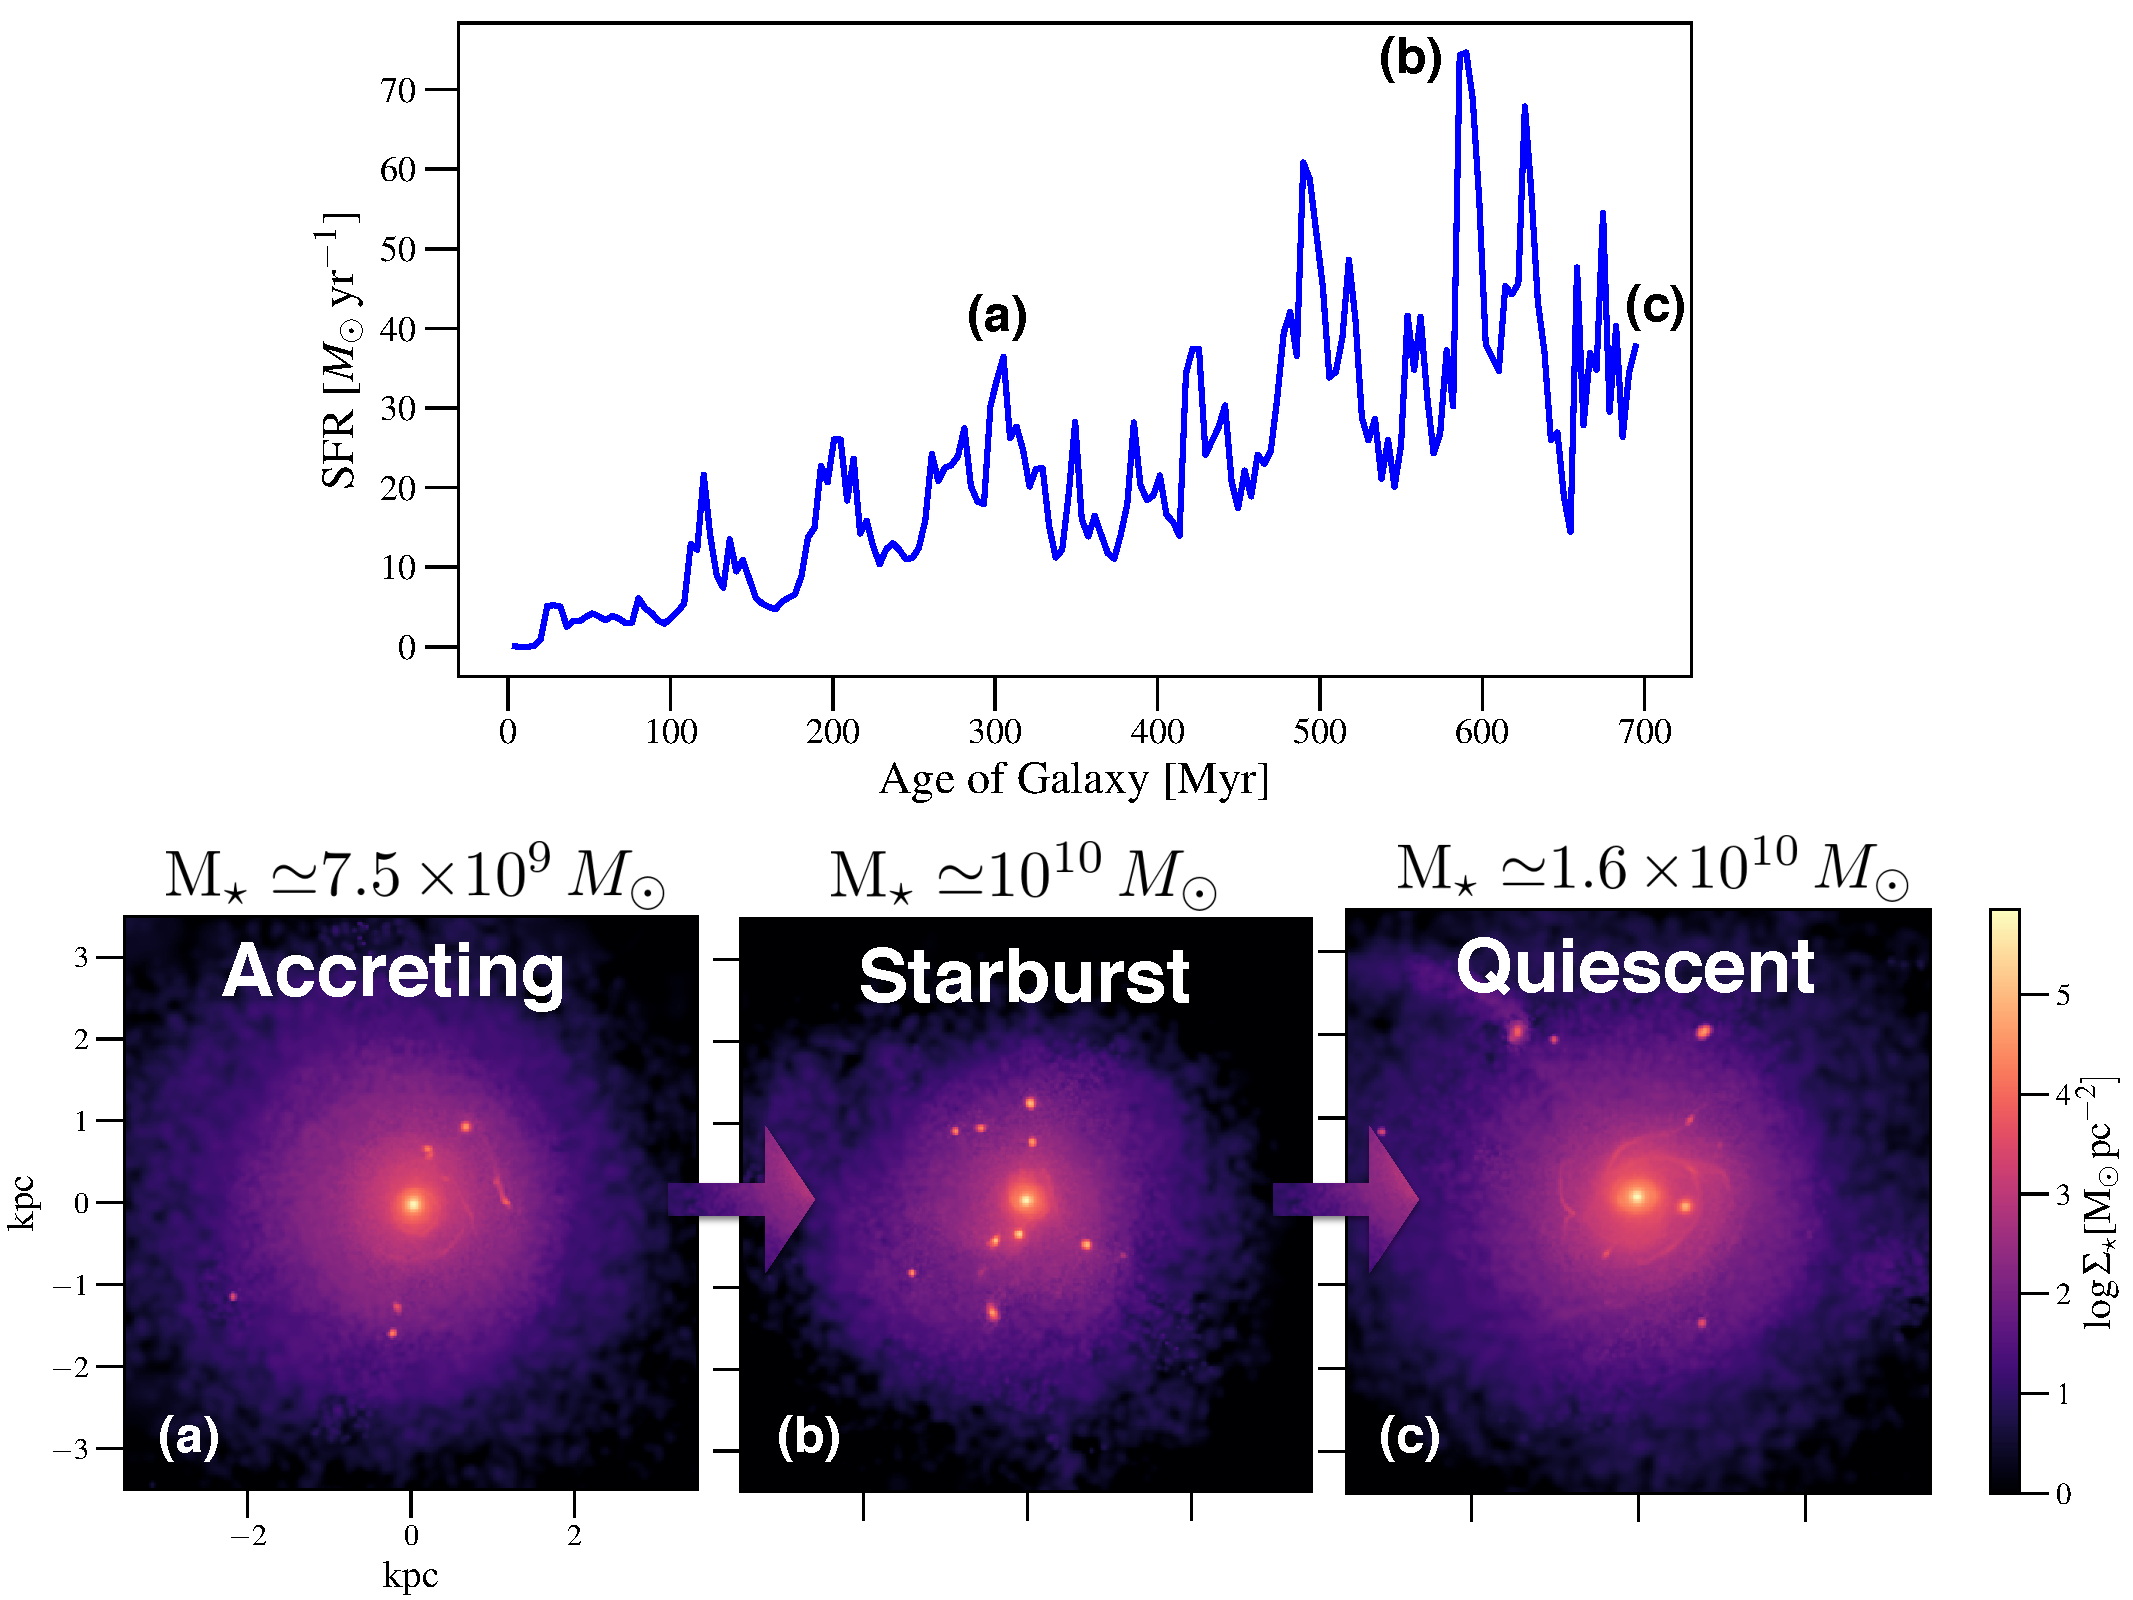
\includegraphics[trim=10 0 0 0, clip, width=0.65\textwidth]{\figpath/sfh.pdf}
\caption{
	Star formation history of \flower (top right) and
	projected stellar mass distribution of \flower during one of its accretion phases
	at its early stage of evolution {\it (a)}; during one of its major starburst phases
	after a major merger {\it (b)}; and in a relatively quiescent phase post-starburst {\it (c)}.
% f_gas history?
\label{fig:SFH}}
\end{figure*}


\subsection{Structure identification} \label{sec:method}
To identify the molecular complexes, we use a customized version of the clump finder algorithm available in the \ncode{python} package \ncode{yt} \citep{Turk2011a}, which was initially described in \citet{Smith09a}, but this function has been modified since then.
%
The latest version of the default \ncode{yt} clump finder decomposes the zones in the simulation into non-overlapping tiles, which are stored in a k-dimensional tree (aka k-d tree). It then identifies the contours of a variable field (here, the density field) within a tile and connects them across the tiles. 
In the customized version used for this study, we modify the function to enhance the stability of the code (which essentially means we fixed the bugs in order for it to actually work).

In the ``clump-finding'' process, we employ a set of different density thresholds defined based on the
molecular hydrogen density of \flower taken at different cosmic times (between $z$\eq6.0\,$-$\,7.2).
We note that this process is in essence similar to
identifying molecular structures based on the noise levels of surface density maps
observers obtain with telescopes, using molecular line tracers such as CO, CS, and HCN,
as commonly adopted in observational studies (e.g., identifying
``clumps'' based on/after applying $\sigma$-clipping,
using tools such as \ncode{aips}'s task \ncode{serch}, \ncode{clumpfind},
and \ncode{cprops}; \citealt{Williams94a, Oka01a, Rosolowsky06a}).
We note that, owing to the nature of \obs, such structures are identified 
in position-position-velocity (PPV) space, whereas in simulations, one has the 
full 6D spatial-kinematic information, and can therefore cleanly identify structures directly using the density field in position-position-position (PPP) space.
% Many concerning the correspondence between  ... , dating back to the work by \citep{Adler92a}.
Existing studies find a good correspondence in the dynamical properties extracted in
PPV- versus PPP-space (\citealt{Ballesteros-Paredes02a, Heitsch09a, Shetty10a, Beaumont13a, 
Pan15a, Ibanez-Mejia16a}, but see also \citealt{Shetty10a} for a discussion on caveats and limitations). 
% large scale structure in PPP may be identified as numerous lower mass structures in the PPV cube due to gradients in the LOS and conversly, superposition when spatially distinct components with the same velocity are "merged" into one component in the PPV space when observed along the LOS (see Fig. 1 of Beaumount13a). (may be worth putting more thoughts on this after the report is due).


\begin{figure}[htbp]
\centering
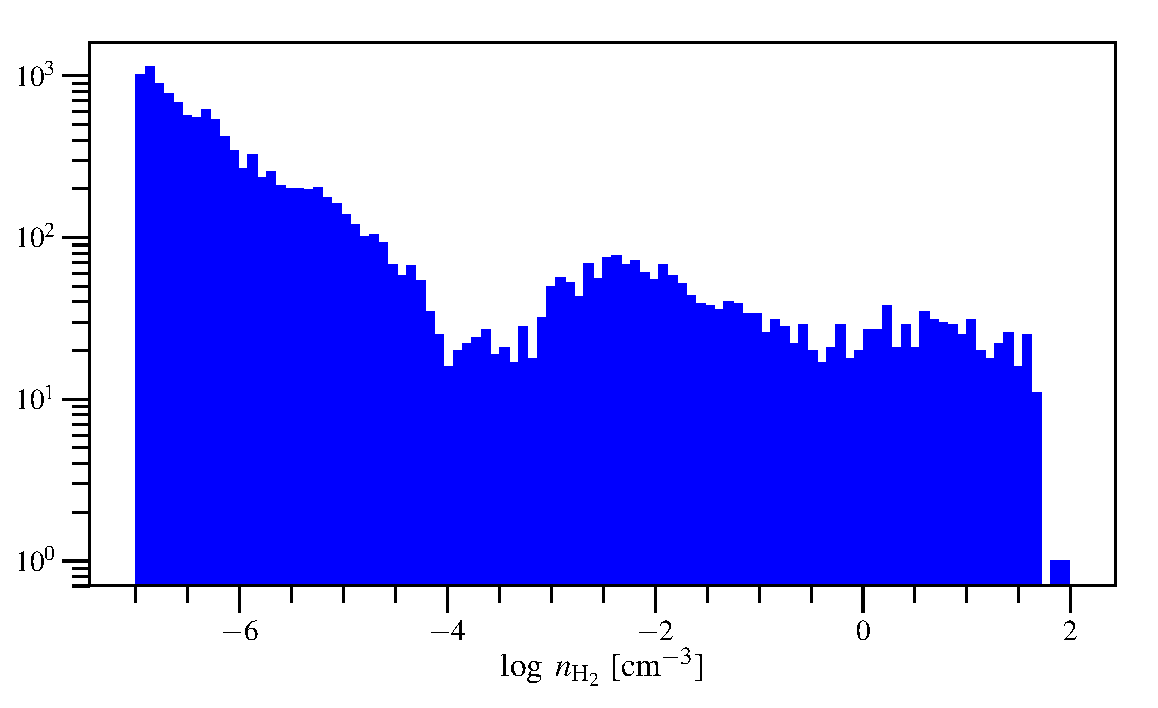
\includegraphics[trim=35 0 10 35, clip, width=0.55\textwidth]{\figpath/hist_test_16.pdf}
\caption{
Volumetric H$_2$ density distribution of \flower taken from a single snapshot, corresponding to the 
accreting phase shown in \Fig{SFH}.
\label{fig:h2density}}
\end{figure}


\begin{figure*}[htbp]
 \centering
  \includegraphics[scale=0.65]{\figpath/{dual_16_ncut_0.53}.png}
  \\[-5.5em]
  \includegraphics[scale=0.65]{\figpath/{dual_16_ncut_6.81}.png}
  \\[-5.5em]
  \includegraphics[scale=0.65]{\figpath/{dual_16_ncut_18.96}.png}
\caption{
MC identified by applying
volumetric H$_2$ density cuts of
$n_{\rm cut}$\eq[0.32, 0.53, 0.88, 1.45, 2.45, 4.08, 6.81, 11.36, 19.00, 31.62]\,cm$^{-3}$.
	Color shows the projected H$_2$ surface density. {\bf this should be H2 density 1/cm$^{-2}$?!} \AP{if i recall correctly, this is not the projected h2 density, but the mass averaged h2 density field; additionally, we should convince yt to plot a proper label for the colorbar, and remove the trailing right axes labels (that are still there despite our efforts)}\DL{I tried more on Sept 7th, errrr, now all the ticks and labels for both panels disappear... hmm.. Not worth my time to fix this for the report.}
% yt.OffAxisProjectionPlot: weight the requested field by the weighting field and integrate along the line of sight.
\label{fig:MC}}
% \addtocounter{figure}{-1}
\end{figure*}

In \Fig{h2density}, we show an example of the volumetric H$_2$ density ($n_{\rm H2}$) distribution of \flower
for a given snapshot which includes contributions from its surrounding 7\,kpc (in diameter)\footnote{For reference,
the half mass radius of \flower is $\sim$0.5\,kpc and the dark matter ``virial radius'' at which the mean enclosed density is 200 times 
the critical density of the Universe % presumably defined at the redshift of \flower here?
is $r_{\rm 200}$\ssim15\,kpc.}.
We note that the distribution is almost flat for $n_{\rm H2}\gtrsim1\,\cc$ and it samples the range of density 
where ``clumps/structures'' are 
found based on the Euler characteristic, i.e., the fourth Minkowsky functional (see calculation presented by \citealt{Pallottini17b}).
In \Fig{MC}, we show an example of the molecular structures identified by applying volumetric H$_2$ density cuts of 
$n_{\rm cut}$\eq[0.32, 0.53, 0.88, 1.45, 2.45, 4.08, 6.81, 11.36, 19.00, 31.62]\,cm$^{-3}$\footnote{Based on 10$^n$, where $n$ represents the 10 elements that are uniformly spaced between [$-0.5, 1.5$] in linear space.
We also vary the range of
$n_{\rm cut}$ adopted and find no qualitative differences
affecting the results and conclusions of this work except in the slope of the CMF (see \Sec{ncut} and \Sec{cmf}).}
to the same snapshot as that
used to plot \Fig{h2density}.
Since the molecular structures identified could
easily appear as overlapping structures depending on the viewing angle, we
also plot them in different three-dimensional projections --- so that one can more
easily see that they are collections of disjoint structures.
We repeat this identification process for 14 snapshots between
redshift \z$\in$[6.0, 7.2], spaced by $\Delta t$\eq50\,Myr.


Limited by the spatial resolution of our simulation ($l_{\rm cell}\simeq$\,30\,pc), we impose an addition constraint such that an identified structure only survives if it spans at least 10 cells in PPP space. We caution that one caveats of such constraint is that we can only examine the parameter space of ``cloud'' scaling relations at ``cloud'' size $R\gtrsim100$\,pc.


\section{Results}     \label{sec:results}


\subsection{Cloud Scaling Relations}

\AP{I see 2 main possible approaches to the presentation of the results
%
(a) focus on a single snapshot, analyze the cloud scaling relation by varying the cuts and then by varying the snapshot; after that one can discuss the stability/toomre analysis of the clumps (help in discussing the origin) and the CMF.
%
(b) discuss each scaling relation one at a time; probabily an introductionary subsection is needed to explain that different cuts yields no qualitative differences.
%
Note that -- in both cases -- alternatively toomre analysis can be done at the beginning of the result section(s).
%
I think that (b) might be a little bit more appealing, since all the plot with similar quantities (e.g. the larson relation for multiple cuts and snapshots) are in the same place (or, even better, page).
}
\DL{agreed, but will move things around later, after the report and after most of the content is ready.}

Molecular clouds are the natal place for \SF, and thus,
their structure and dynamics hold important clues to understanding
the mechanisms and physics of formation and evolution of molecular structures and \SF.
Upon identifying the molecular structures, we extract parameters such as
the virial parameter ($\alpha_{\rm vir}$),
the ``cloud'' mass ($M_{\rm cl}$),
the ``cloud'' size ($R$),
the Mach number ($\mathcal{M}$),
the velocity dispersion ($\sigma$), and the
gas surface density ($\Sigma_{\rm gas}$)
to examine their dynamics.

The mass of an MC is calculated from the uniformly-gridded 3D density field,
integrating over all zones of the MC, multiplied by its volume. 
The size of an MC ($R$) is defined assuming spherical geometry (i.e., 
the size is parameterized via the radius of a sphere, which has a volume corresponding to that of the identified MC).
Since in \obs, dense gas contributes more to the observed linewidths than the more diffuse gas. We therefore calculate 
the one-dimensional non-thermal component of the velocity dispersion ($\sigma_{\rm NT}$) of each MC as a density-weighted quantity:
\begin{equation}
\sigma_{\rm NT}^2 = \frac{1}{{3}}\frac{\sum_{xyz} \sum_{i}^N \rho_i \left(\mathbf{v} - \mathbf{\bar v}\right)_{xyz}^2}{\sum_i^N \rho_i},
\end{equation}
where $N$ is the number of zones of each MC.
The total velocity dispersion includes contributions from the thermal sound speed ($c_s$):
\begin{equation}
\sigma^2 = \sigma_{\rm NT}^2 + c_s^2.
\end{equation}
The local sound speed ($c_s$)
of all identified molecular complexes are generally much smaller compared to the their
turbulent velocities.
\AP{i would put the following as a footnote or this point might be moved; alternatively these points (see also the emails) can be treated when dealing with the stability analysis}
We find comparable velocity dispersion derived by taking the root mean square versus
that derived using thermal and non-thermal pressure, indicating that
rotation velocity is unlikely to be the dominant source entering the velocity dispersion reported here.
We quantify the contributions arising from galactic rotation and shear to the extracted velocity dispersions of the MCs in \Sec{Q}.
In the subsequent sections, we adopt the root mean square of the velocity field
as the velocity dispersion ($\sigma$).


We show in \Fig{dist} the MC distributions in terms of their
molecular gas masses, radii, gas mass fraction ($f_{\rm gas}$\eq$M_{\rm gas}$/($M_{\rm gas}$ +
$M_*$)).
We note that the distributions vary for different snapshots, depending on the evolutionary stage of \flower.
The highest surface density threshold of $n_{\rm cut}$ yields a ``minimum'' MC mass on
the order of 10$^{6.5}$\,\Msun for the densest MC identified.
We find $\sim$10$-$13 MCs with masses exceeding 10$^8$\,\Msun across all the
snapshots for each of the given $n_{\rm cut}$ (see \Sec{method}).

\begin{figure*}[htbp]
\centering
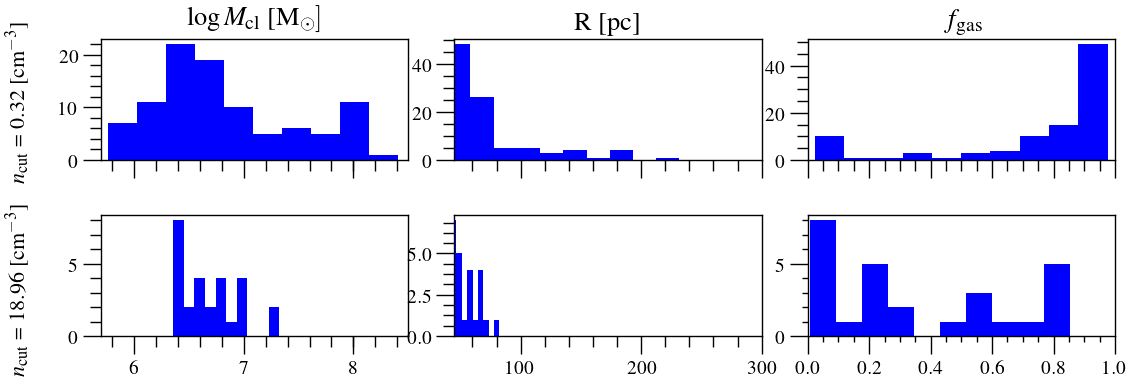
\includegraphics[trim=0 0 0 0, clip, width=0.85\textwidth]{\figpath/minmaxNcut_basicDistributions.png}
\caption{
Distributions of masses, sizes, and gas mass fractions of MCs identified using 
the lowest $n_{\rm cut}$ (left panels) and the highest $n_{\rm ncut}$ (right panels).
Note the y-axis scales are different between the left and the right panels, as less MCs are identified 
at higher $n_{\rm cut}$.
\label{fig:dist}}
\end{figure*}




In the following subsections,
we examine the MC properties in the context of the Larson's relations \citep{Larson81a}, which
describe interactions between gravity and turbulence and is the first set of 
relations used for studying star-forming molecular structure formation based on observables (linewidth-size,
density-size, and mass-size relations) and for comparing properties of molecular structures
in different galactic environments.
% Inner MW: R=2-8.5 kpc, most of the mass in the molecular ISM is in the form of GMCs with sizes $gtrsim$20\,pc and masses greater than 10$^5$\,\Msun \citep{Sanders85a}.
Observations of nearby gas-rich galaxies such as M64 and NGC\,253
show higher velocity dispersions compared
to the disk/mid-plane of the Milky Way which
are more consistent with those observed in the inner regions of
Milky Way \citep{Oka01a, Rosolowsky05a, Heyer09a, Leroy15a}.  % also higher $P_{\rm int}$,
% which is $\propto\rho\sigma^2$
While the velocity dispersions of the clouds in these nearby gas-rich galaxies are comparable
to the inner regions of Milky Way, they are found to be bigger in size (approximately
an order of magnitude) and mass (approximately two orders of magnitude).
These bigger clouds have been interpreted as a results of their higher gas mass fractions and
surface densities and velocity dispersions, since
fragmentation occurs near the Jeans length $L_J\propto\sigma^2/\Sigma$
and Jeans mass $M_J\propto\sigma^4/\Sigma$
for dispersion-supported structures.

\subsubsection{Formalism: Virial Equilibrium and Larson's Relations}  \label{sec:PVE}
% Relating Larson's law to stability and pressure (perhaps move this to other section?).
A spherically symmetric cloud of mass $M$ and radius $R$ embedded within
a medium of pressure $P$ is described using the virial theorem:
\begin{equation}
\frac{1}{2}\ddot I = 2(T - T_s) + W + B,
\end{equation}
where $\ddot I$ is the second time derivative of the Lagrangian moment of inertia,
$T$ is the volume term of the total kinetic energy (including thermal and
bulk motions), $T_s$ is the surface term due to external thermal pressure,
$W$ is the gravity term, and $B$ is the magnetic term.
In the case where magnetic field is excluded (i.e., $B$\eq0), we can express this in terms of:
\begin{equation}
\frac{1}{2}\ddot I = 3 M \sigma^2 - \frac{\Gamma GM^2}{R} - 4\pi P_{\rm ext} R,
\label{eqn:virial}
\end{equation}
where the first term on the right hand side (RHS) is the pressure term from velocity dispersion, the second
term is the gravity term, and the third term is the external pressure term.
For the case of simple virial equilibrium (SVE; i.e., equilibrium state without external pressure),
the LHS and the last term on the RHS vanish. The equation becomes:
\begin{equation}
\alpha_{\rm vir} = \frac{3\sigma^2}{\Gamma GM/R} = \frac{5\sigma^2R}{GM},
\end{equation}
where $\Gamma$ is set to 3/5 for a uniform sphere.
We can define
\begin{equation}
V_0^2\equiv\frac{\sigma^2}{R},
\end{equation}
which is related to the scaling in one of the Larson's relations (linewidth-size)
and can be re-written in the form of:
\begin{equation}
\sigma^2/R = \pi G \Sigma/5.
\end{equation}
For pressure-bounded virial equilibrium (PVE; i.e. equilibrium state with pressure), % external pressure
Equation~\ref{eqn:virial} becomes
\begin{equation}
P_{\rm ext} = \frac{3\sigma^2M}{4\pi R^3} - \frac{\Gamma G M^2}{4\pi R^4},
\label{eqn:pext}
\end{equation}
which describes the external pressure needed to confine the gas inside a volume $V$.
Rearranging the equation and substituting $\Sigma$\eq$M/\pi R^2$, we can express
this equation using the following:
\begin{equation}
\frac{\sigma^2}{R} = \frac{1}{3}\left(\frac{4P_{\rm ext}}{\Sigma} + \Gamma G \Sigma \pi \right).
\label{eqn:v0}
\end{equation}
Therefore, for a virialized cloud, one expects a one-to-one mapping between $V_0^2$ and $\Sigma$ since
$\sigma^2/R\propto\Sigma$, whereas
Equation~\ref{eqn:v0} represents the loci along which external pressures $P_{\rm ext}$ are
needed in order for MCs to have linewidths $\sigma$ for a given set of surface densities.
In other words, a cloud with $\sigma$ and $\Sigma$ offset from $\sigma^2/R\rightarrowtail\Sigma$
is in equilibrium with the external pressure (and therefore $V_0^2$ is not constant with $\Sigma$ but
varies depending on $P_{\rm ext}$; cf. expectation for SVE
$\sigma\propto R^{0.5}$; see e.g., \citealt{Heyer09a, Hughes10a, Hughes13b, Meidt13a}).


\subsubsection{Single Snapshots}  \label{sec:singless}

%
\AP{I would move the following when discussing the velocity dispersion; additionally, the large velocity dispersions was also noted in Vallini2018a, we can use some of those results to complement the discussion (e.g. shift for the CO sled at higher J then local galaxies).}

In each snapshot (see \Fig{MC} for example),
we identify a set of MCs with consistently high turbulences and surface densities
regardless of the H$_2$ density cuts adopted.
These are the MCs at the center of the main disk of \flower and
occupy the top right corner of the Larson's relation shown in \Fig{larsons_single}.
\AP{however a plot showing the clump stats has not been show yet at this point}
Their high velocity dispersions and surface densities are expected since
they are located in the nuclear regions of the
galaxy, where the potential well is also deeper. The higher velocity dispersions
in these MCs can also be understood as they have experienced more recent episodes
of \SF as \flower is assembling its stellar mass (they also have higher stellar-to-gas mass ratios of $\sim$60).
In fact, by $z\simeq$7.2 (i.e., the snapshot corresponding
to the top panel of \Fig{SFH} and \Fig{larsons_single}), \flower has assembled
a stellar mass of $M_*$\eq7.5\E{9}\,\Msun. Thus, the higher velocity dispersion
is due in part to the stronger stellar feedback compared to e.g., MCs in its satellite galaxies.
Based on the virial parameter, the MC identified in (the densest region of) the main disk of \flower
would indicate that the MC itself is gravitationally unbound, and is supported/confined 
by turbulence and rotation on large scales.
% clouds form in galactic disk typically have virial between 0.2-10 \citep{Dobbs08a, Tasker09a}.

As we increase the density threshold, some of the MC within the main disk break
into multiple sub-MCs.
As such, we effectively identify a population of denser molecular structures  (\Fig{MC}).
\AP{the following will be manifest only after the presentation of some results, e.g. \Fig{alpha16}}
This population of sub-MCs has dynamics largely
similar to those observed
in $z$\ssim2 spatially resolved studies of gas-rich SFGs, in
terms of their velocity dispersions, sizes, and gas surface densities (\Fig{larsons_single}; see
e.g., \citealt{Swinbank11a}),
with cloud sizes on the order of $R\simeq$100\,pc and velocity
dispersions of $\sigma\simeq$\,20$-$\,80\,\kms. Their $\alpha_{\rm vir}$
are lower than their ``parent'' MCs in the main disk of \flower. This is consistent with
the conventional wisdom that collapsing structures result from local gravitational
instability within globally non-collapsing structures,
which are supported by turbulence and rotation.
These 

We also identify MCs in the satellite galaxies of \flower. These MCs
tend to have lower velocity dispersions compared to those of \flower which are more comparable
to those observed in the inner Milky way and
nearby gas-rich galaxies (e.g., M64; \citealt{Oka01a, Rosolowsky05a, Heyer09a}),
along the locus of $\sigma\propto R^{0.56}$.
These MCs in the satellite galaxies also have
lower virial parameters compared to the (sub-)MCs in the main disk of \flower,
with $\alpha_{\rm vir}\simeq$1 (see top panels of \Fig{alpha16} and \Fig{alpha27}).
Differences in their $\alpha_{\rm vir}$ most likely result from the weaker
stellar feedback in the satellite galaxies as they have experienced less episodes of \SF compared to
\flower (i.e., lower stellar-to-gas mass ratios of $\sim$0.1). Given their low $\alpha_{\rm vir}$ parameter,
these structures are likely collapsing structures.
Based on the $\sigma^2/R - \Sigma$ relation and the virial parameter,
the MCs of the satellite galaxies of
\flower are close to being in virial equilibrium and are unlikely supported against collapse by external pressure. 


\begin{figure*}[htbp]
\centering
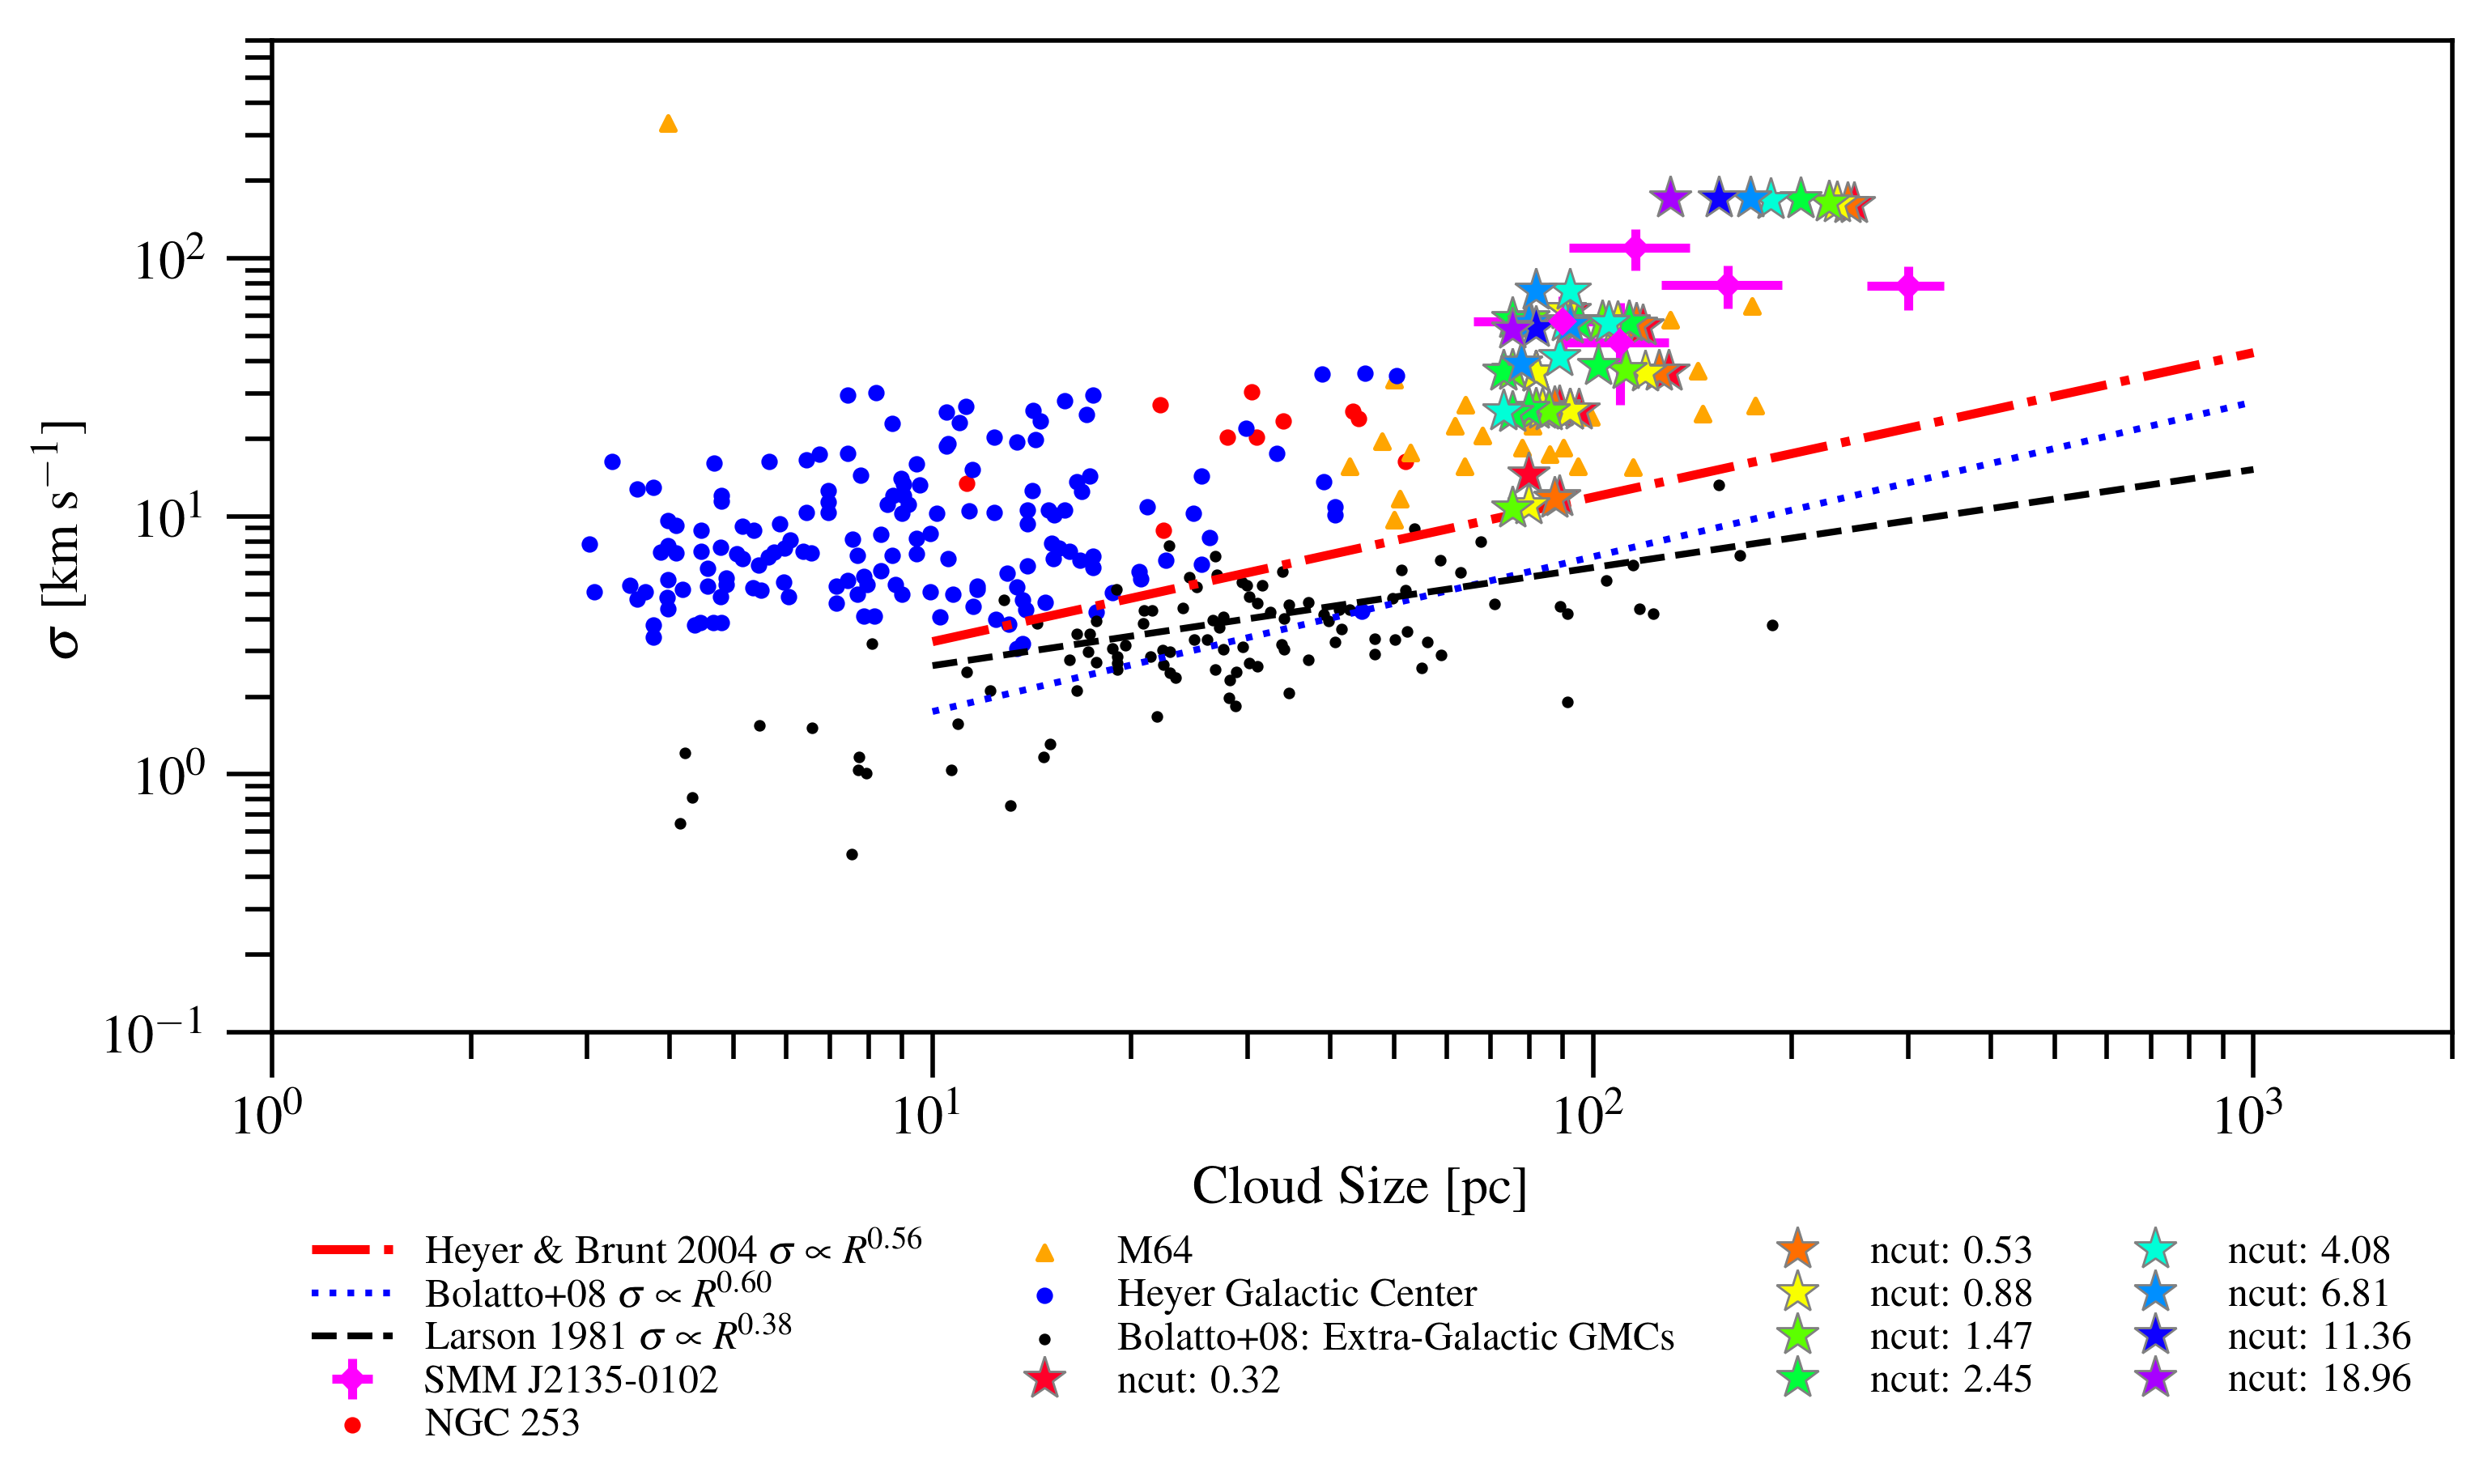
\includegraphics[trim=0 0 0 0, clip, width=0.85\textwidth]{\figpath/ss16_larsons.png}
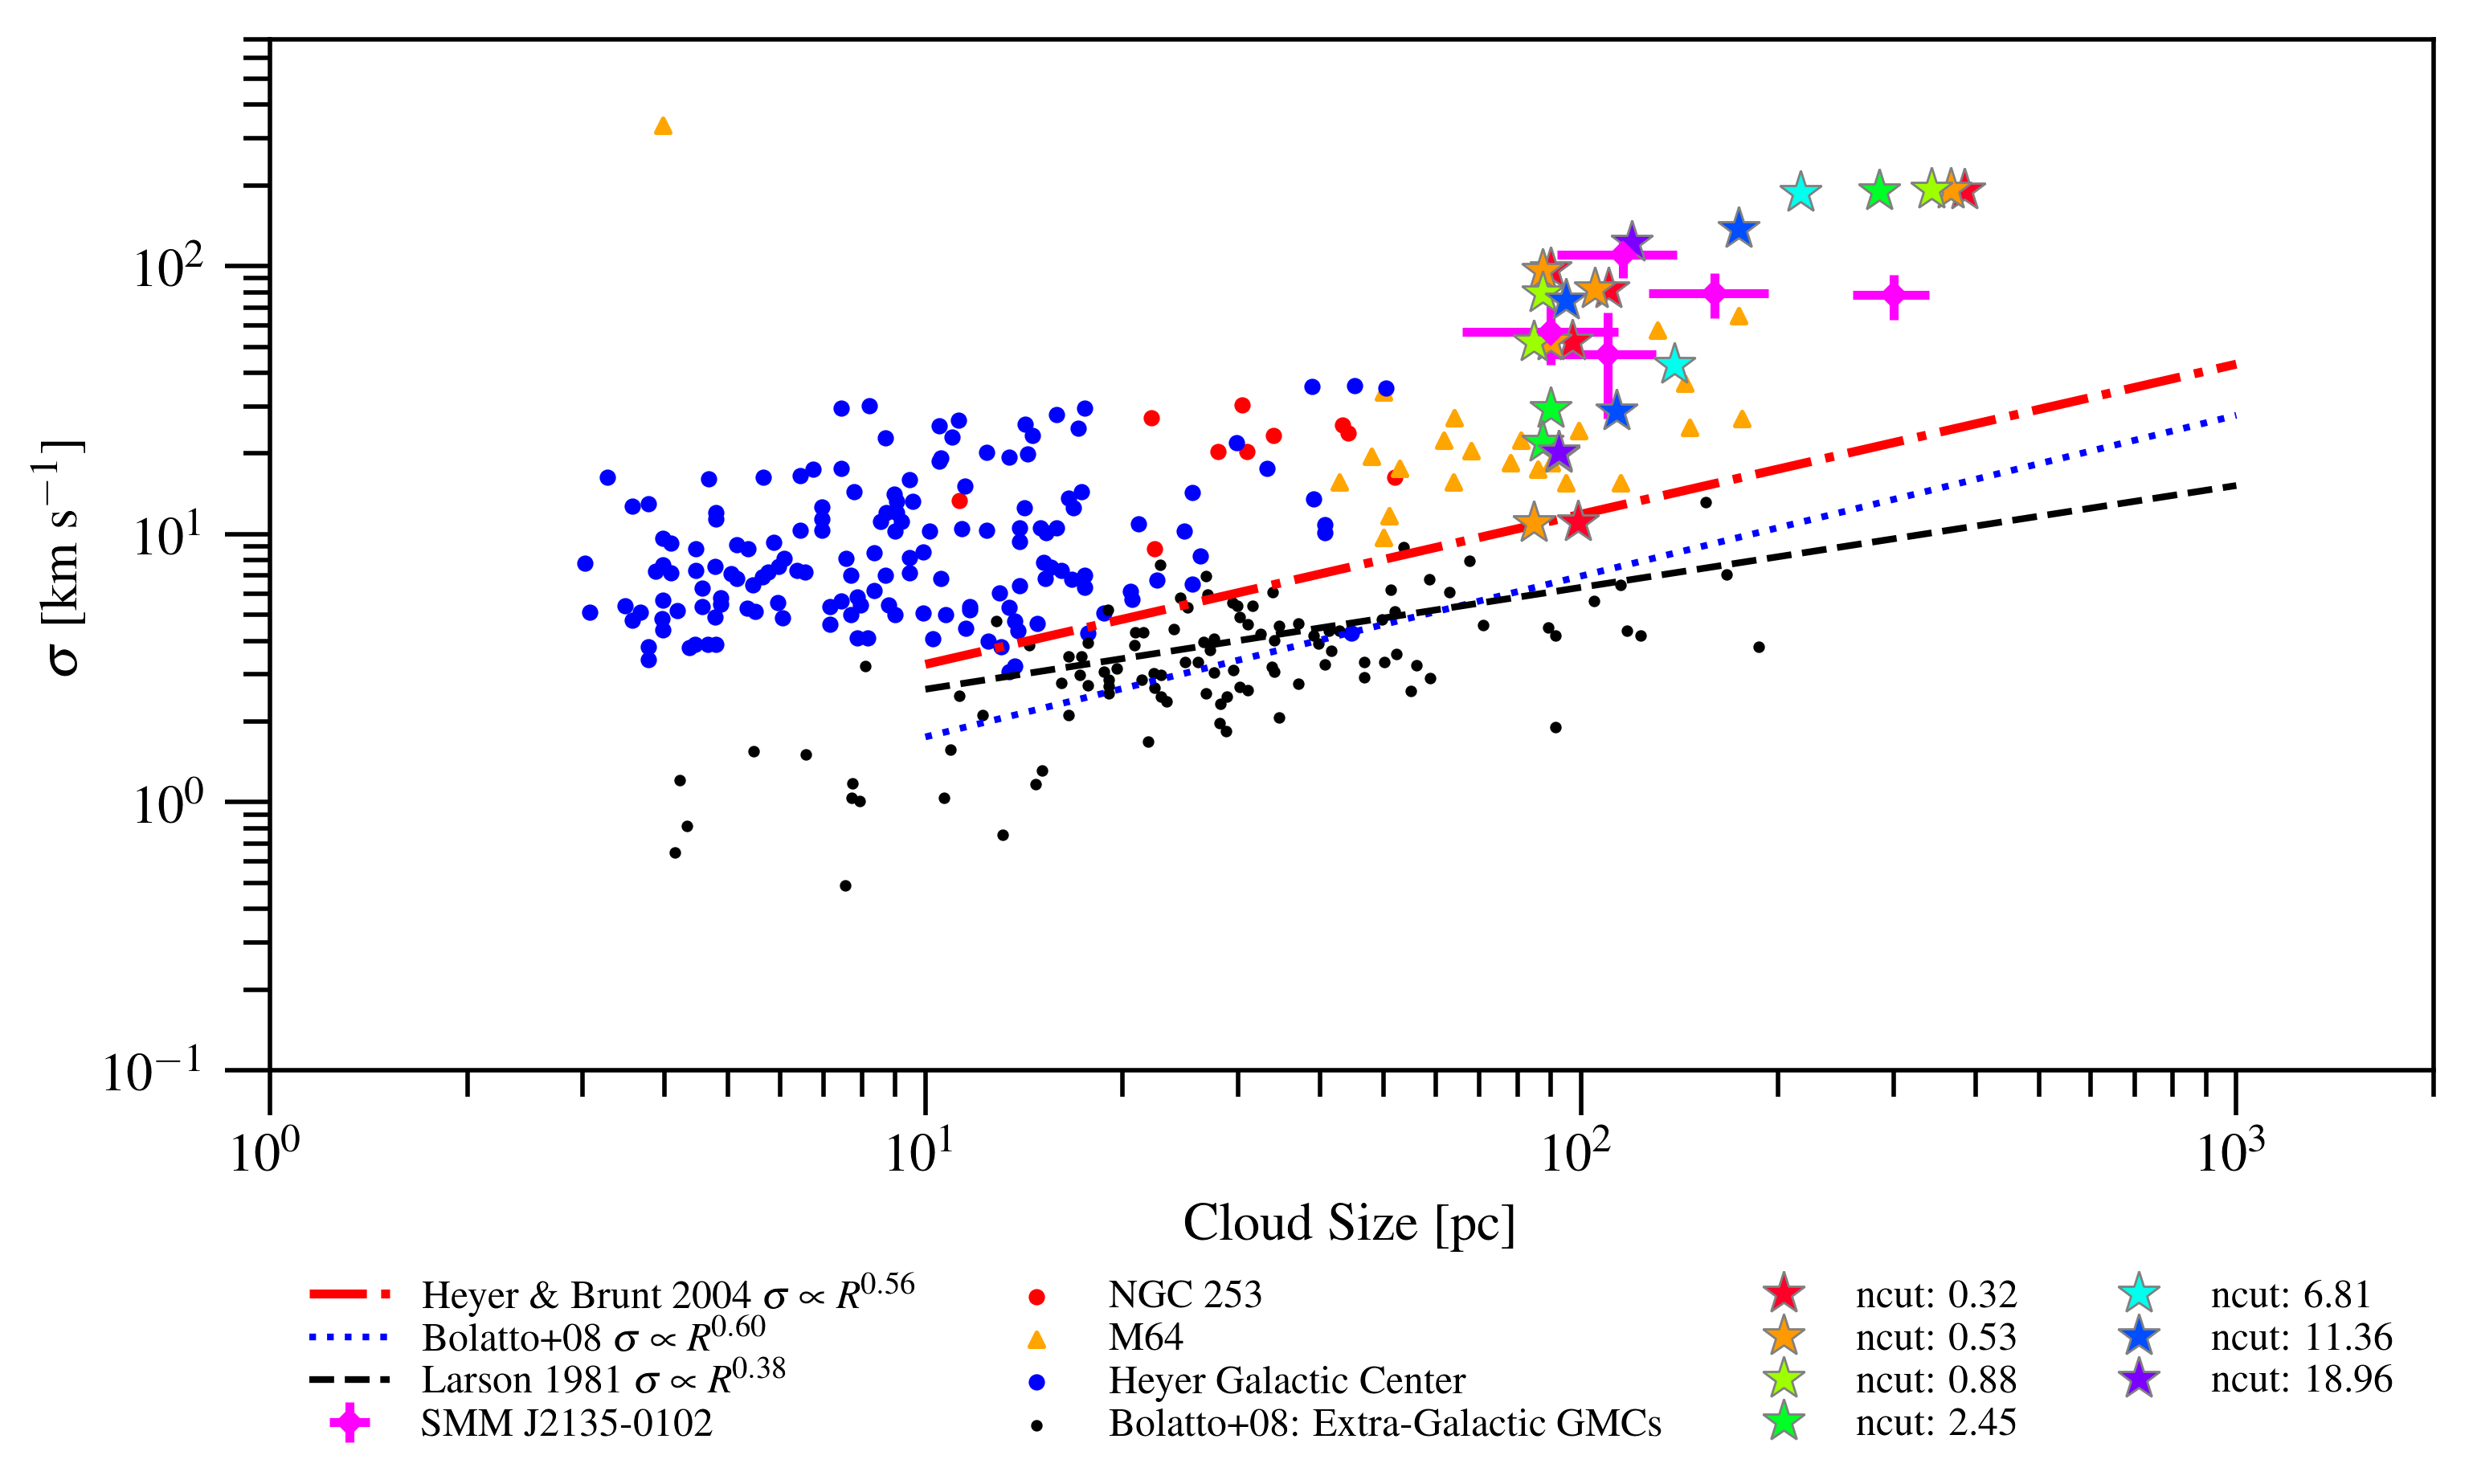
\includegraphics[trim=0 0 0 0, clip, width=0.85\textwidth]{\figpath/ss27_larsons.png}
\caption{
Larson's (linewidth-size) relation of \flower in
accreting phase (top) and
starburst phase (bottom) compared to
those observed in nearby and the \z$\sim$2 star-forming galaxy.
\label{fig:larsons_single}}
\end{figure*}


\begin{figure*}[htbp]
\centering
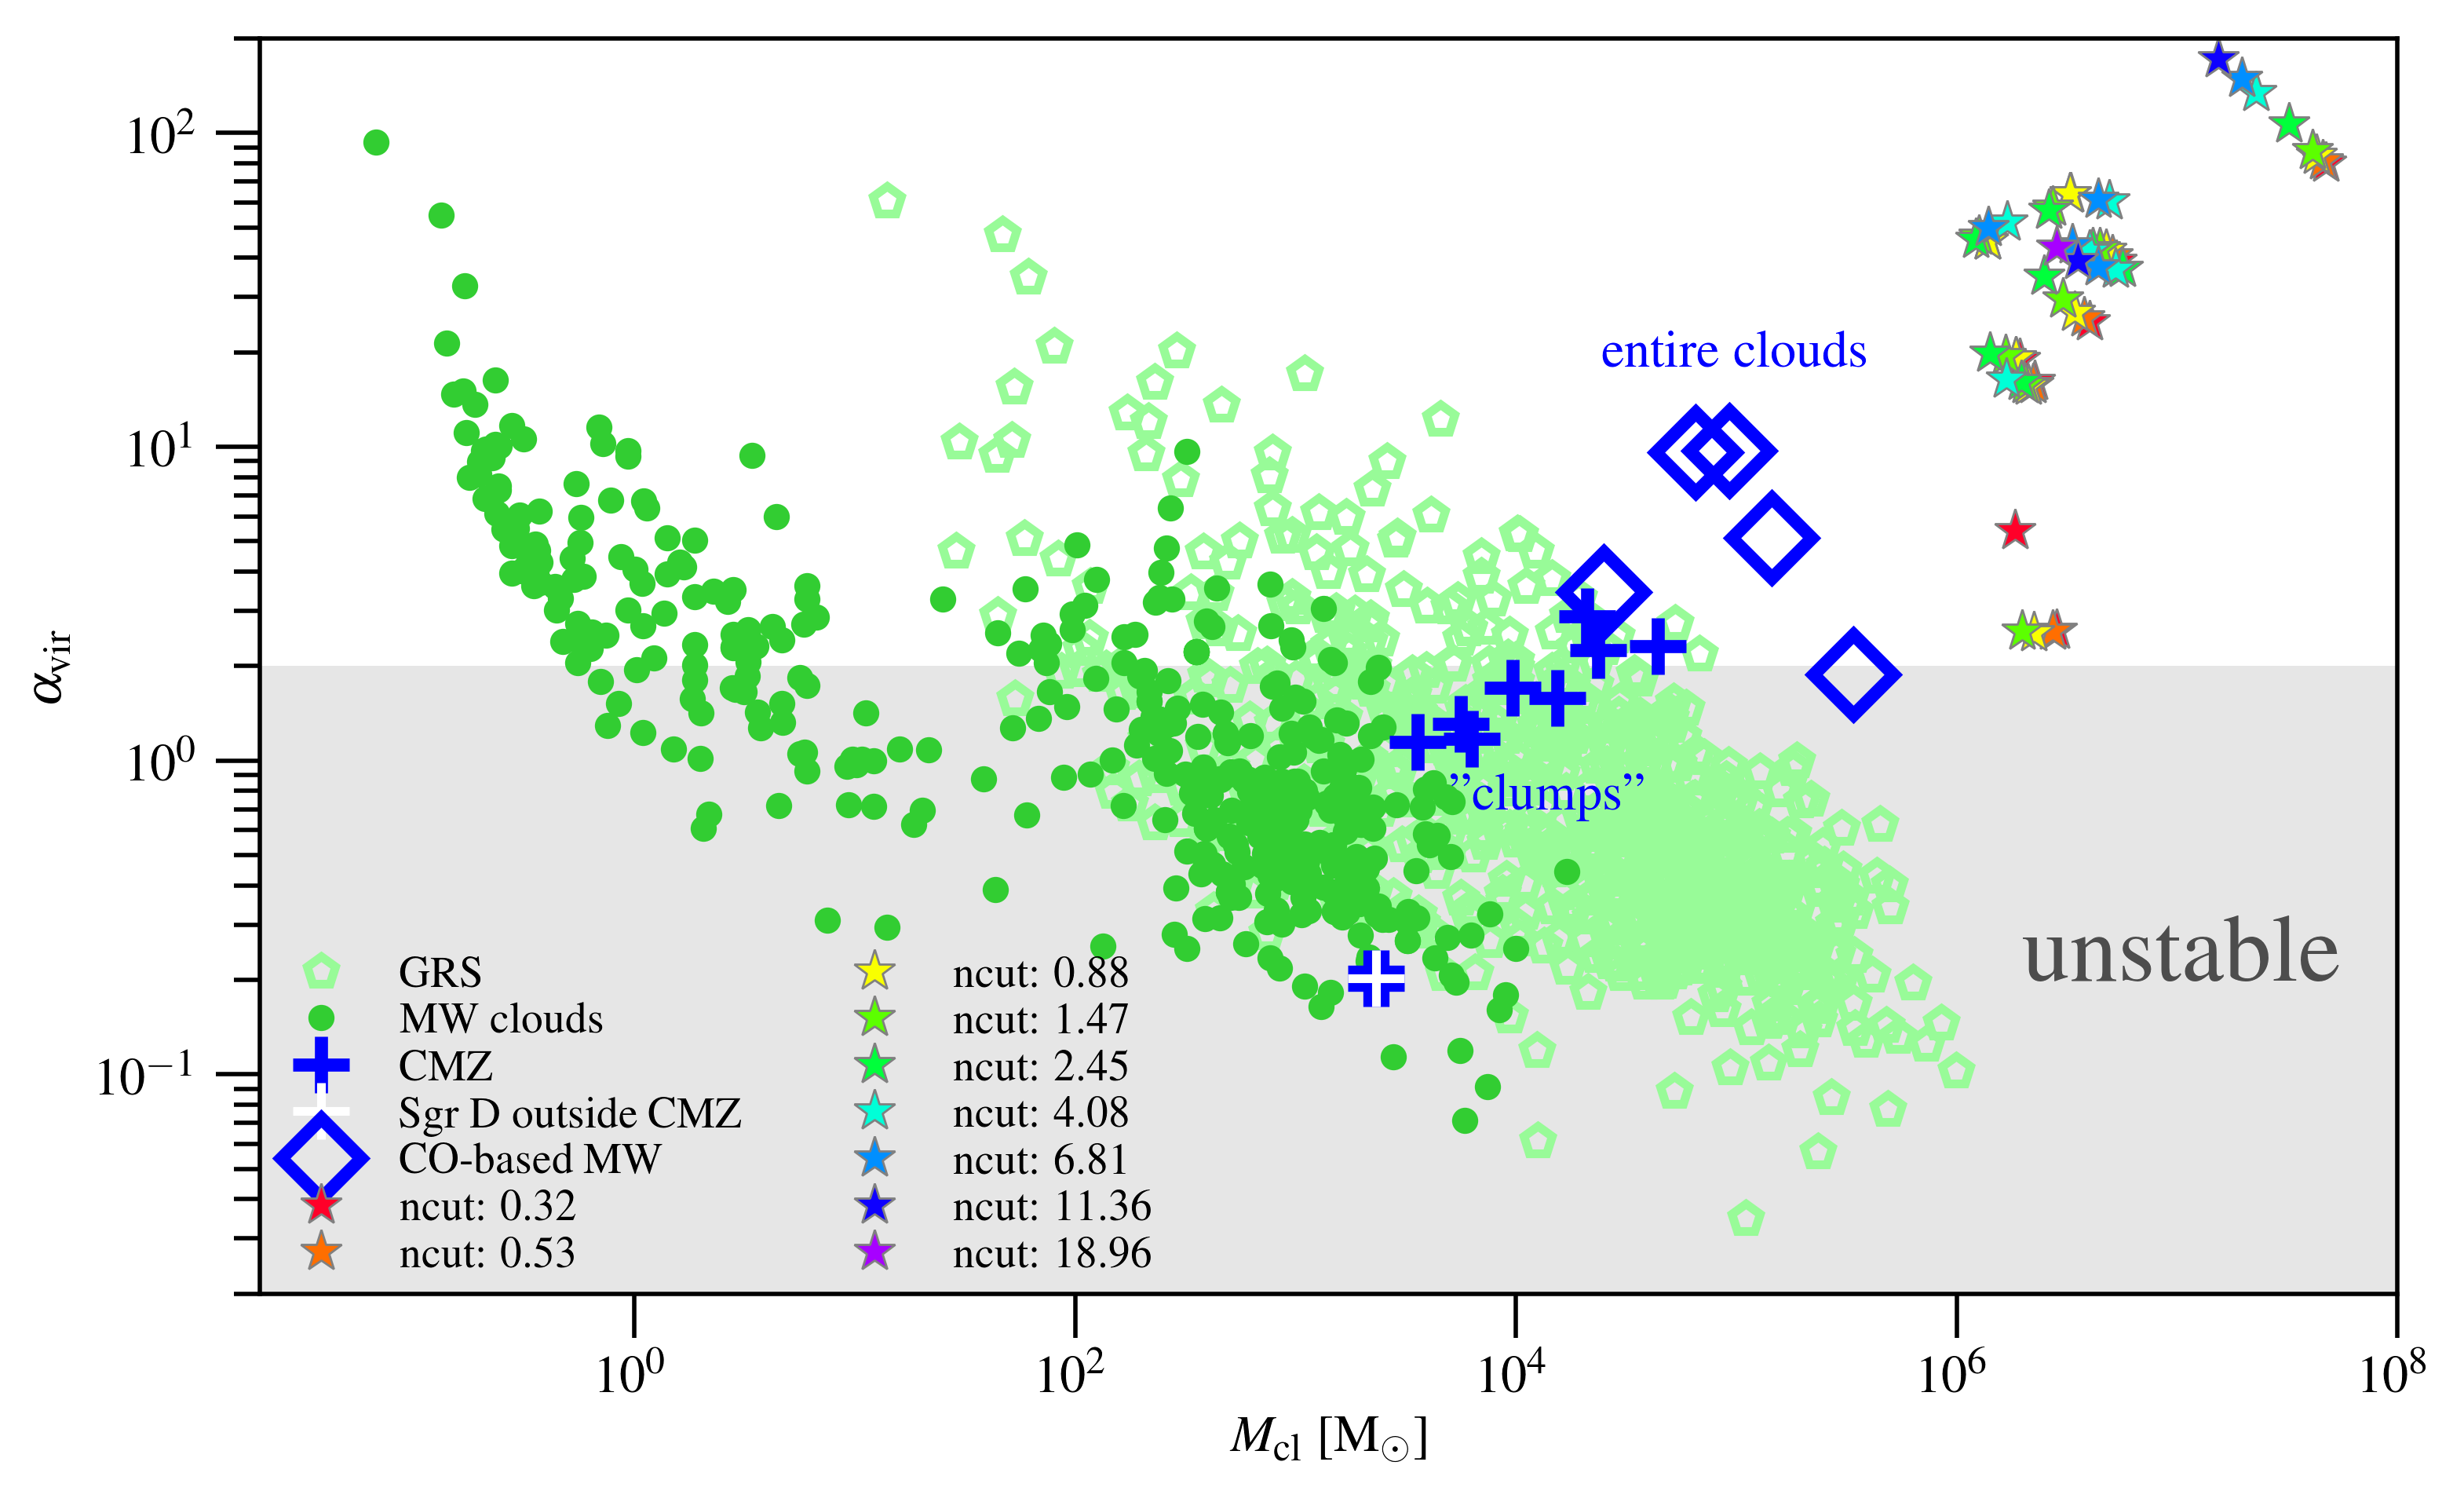
\includegraphics[trim=0 0 0 0, clip, width=0.85\textwidth]{\figpath/ss16_alphavir.png}
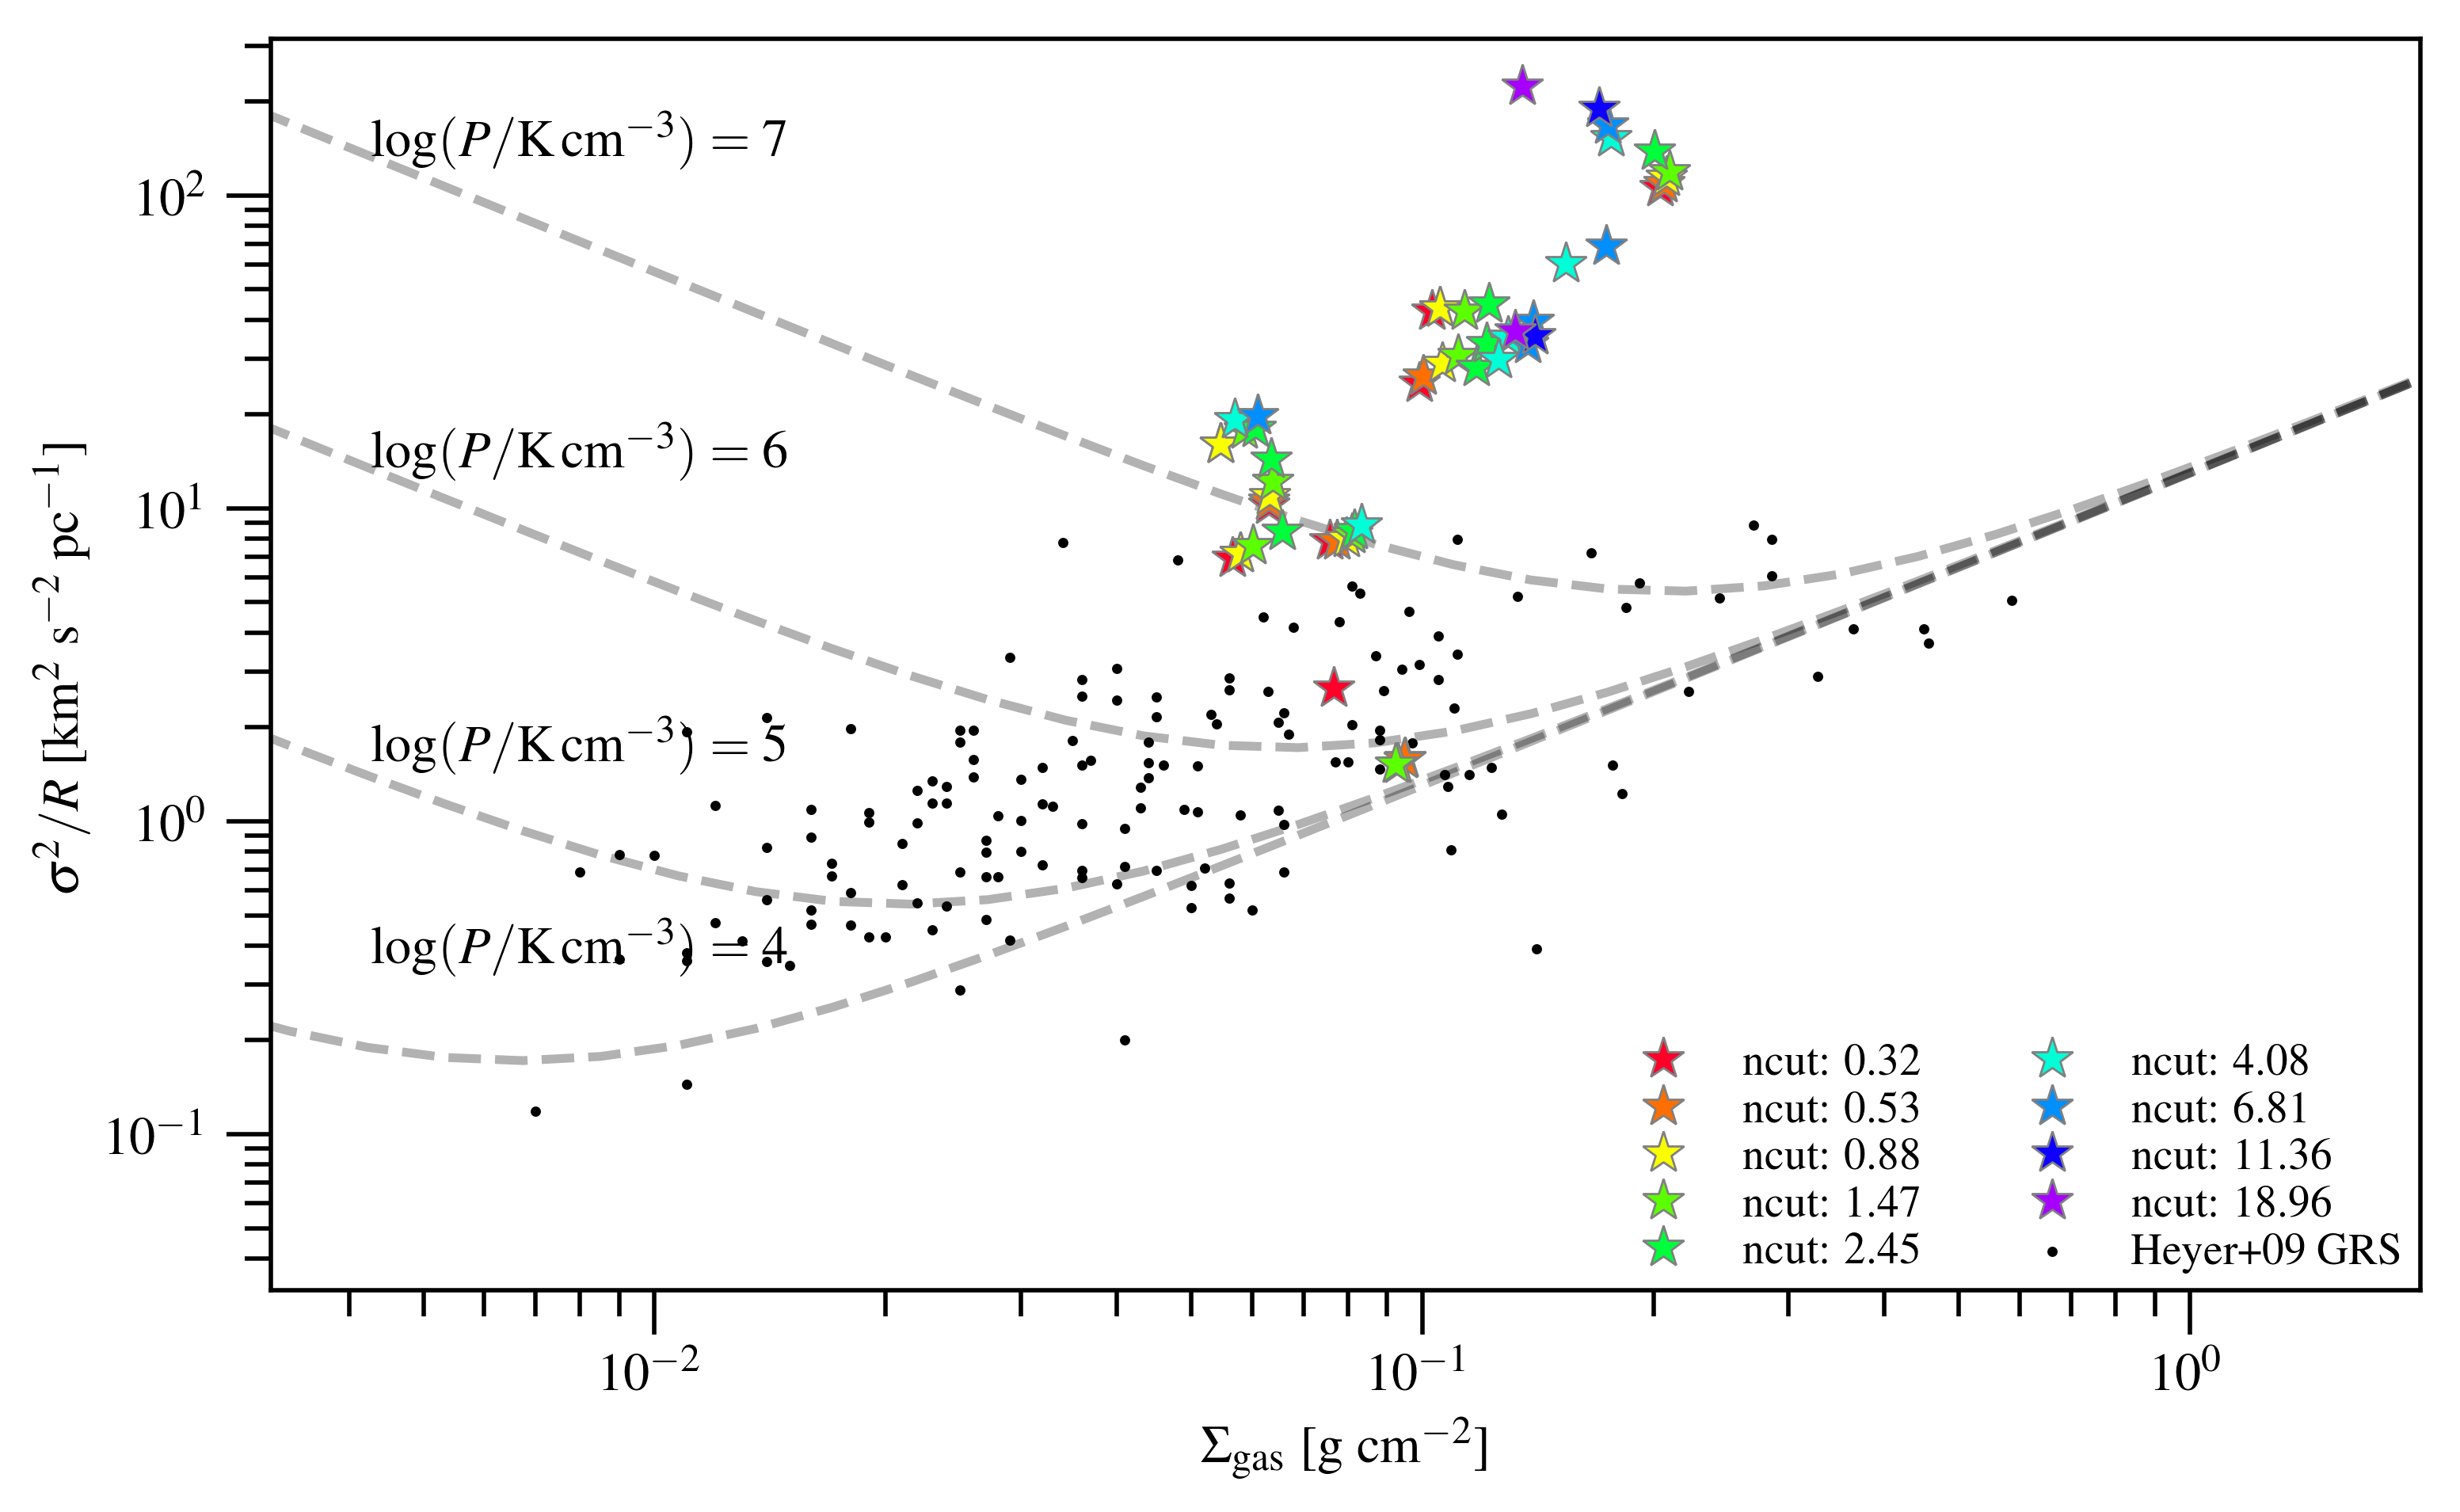
\includegraphics[trim=0 0 0 0, clip, width=0.85\textwidth]{\figpath/ss16_PVE.png}
\caption{
Top: Virial parameter and cloud mass of \flower of a given snapshot (accreting phase).
Bottom: $\sigma^2/R - \Sigma_{\rm gas}$ relation of MCs in the same snapshot.
The V-shaped dashed lines show locii along which the given external pressures
are needed in order for MCs to have linewidth $\sigma$ for a given set of surface densities. (see \Sec{PVE})
\label{fig:alpha16}}
\end{figure*}


\begin{figure*}[htbp]
\centering
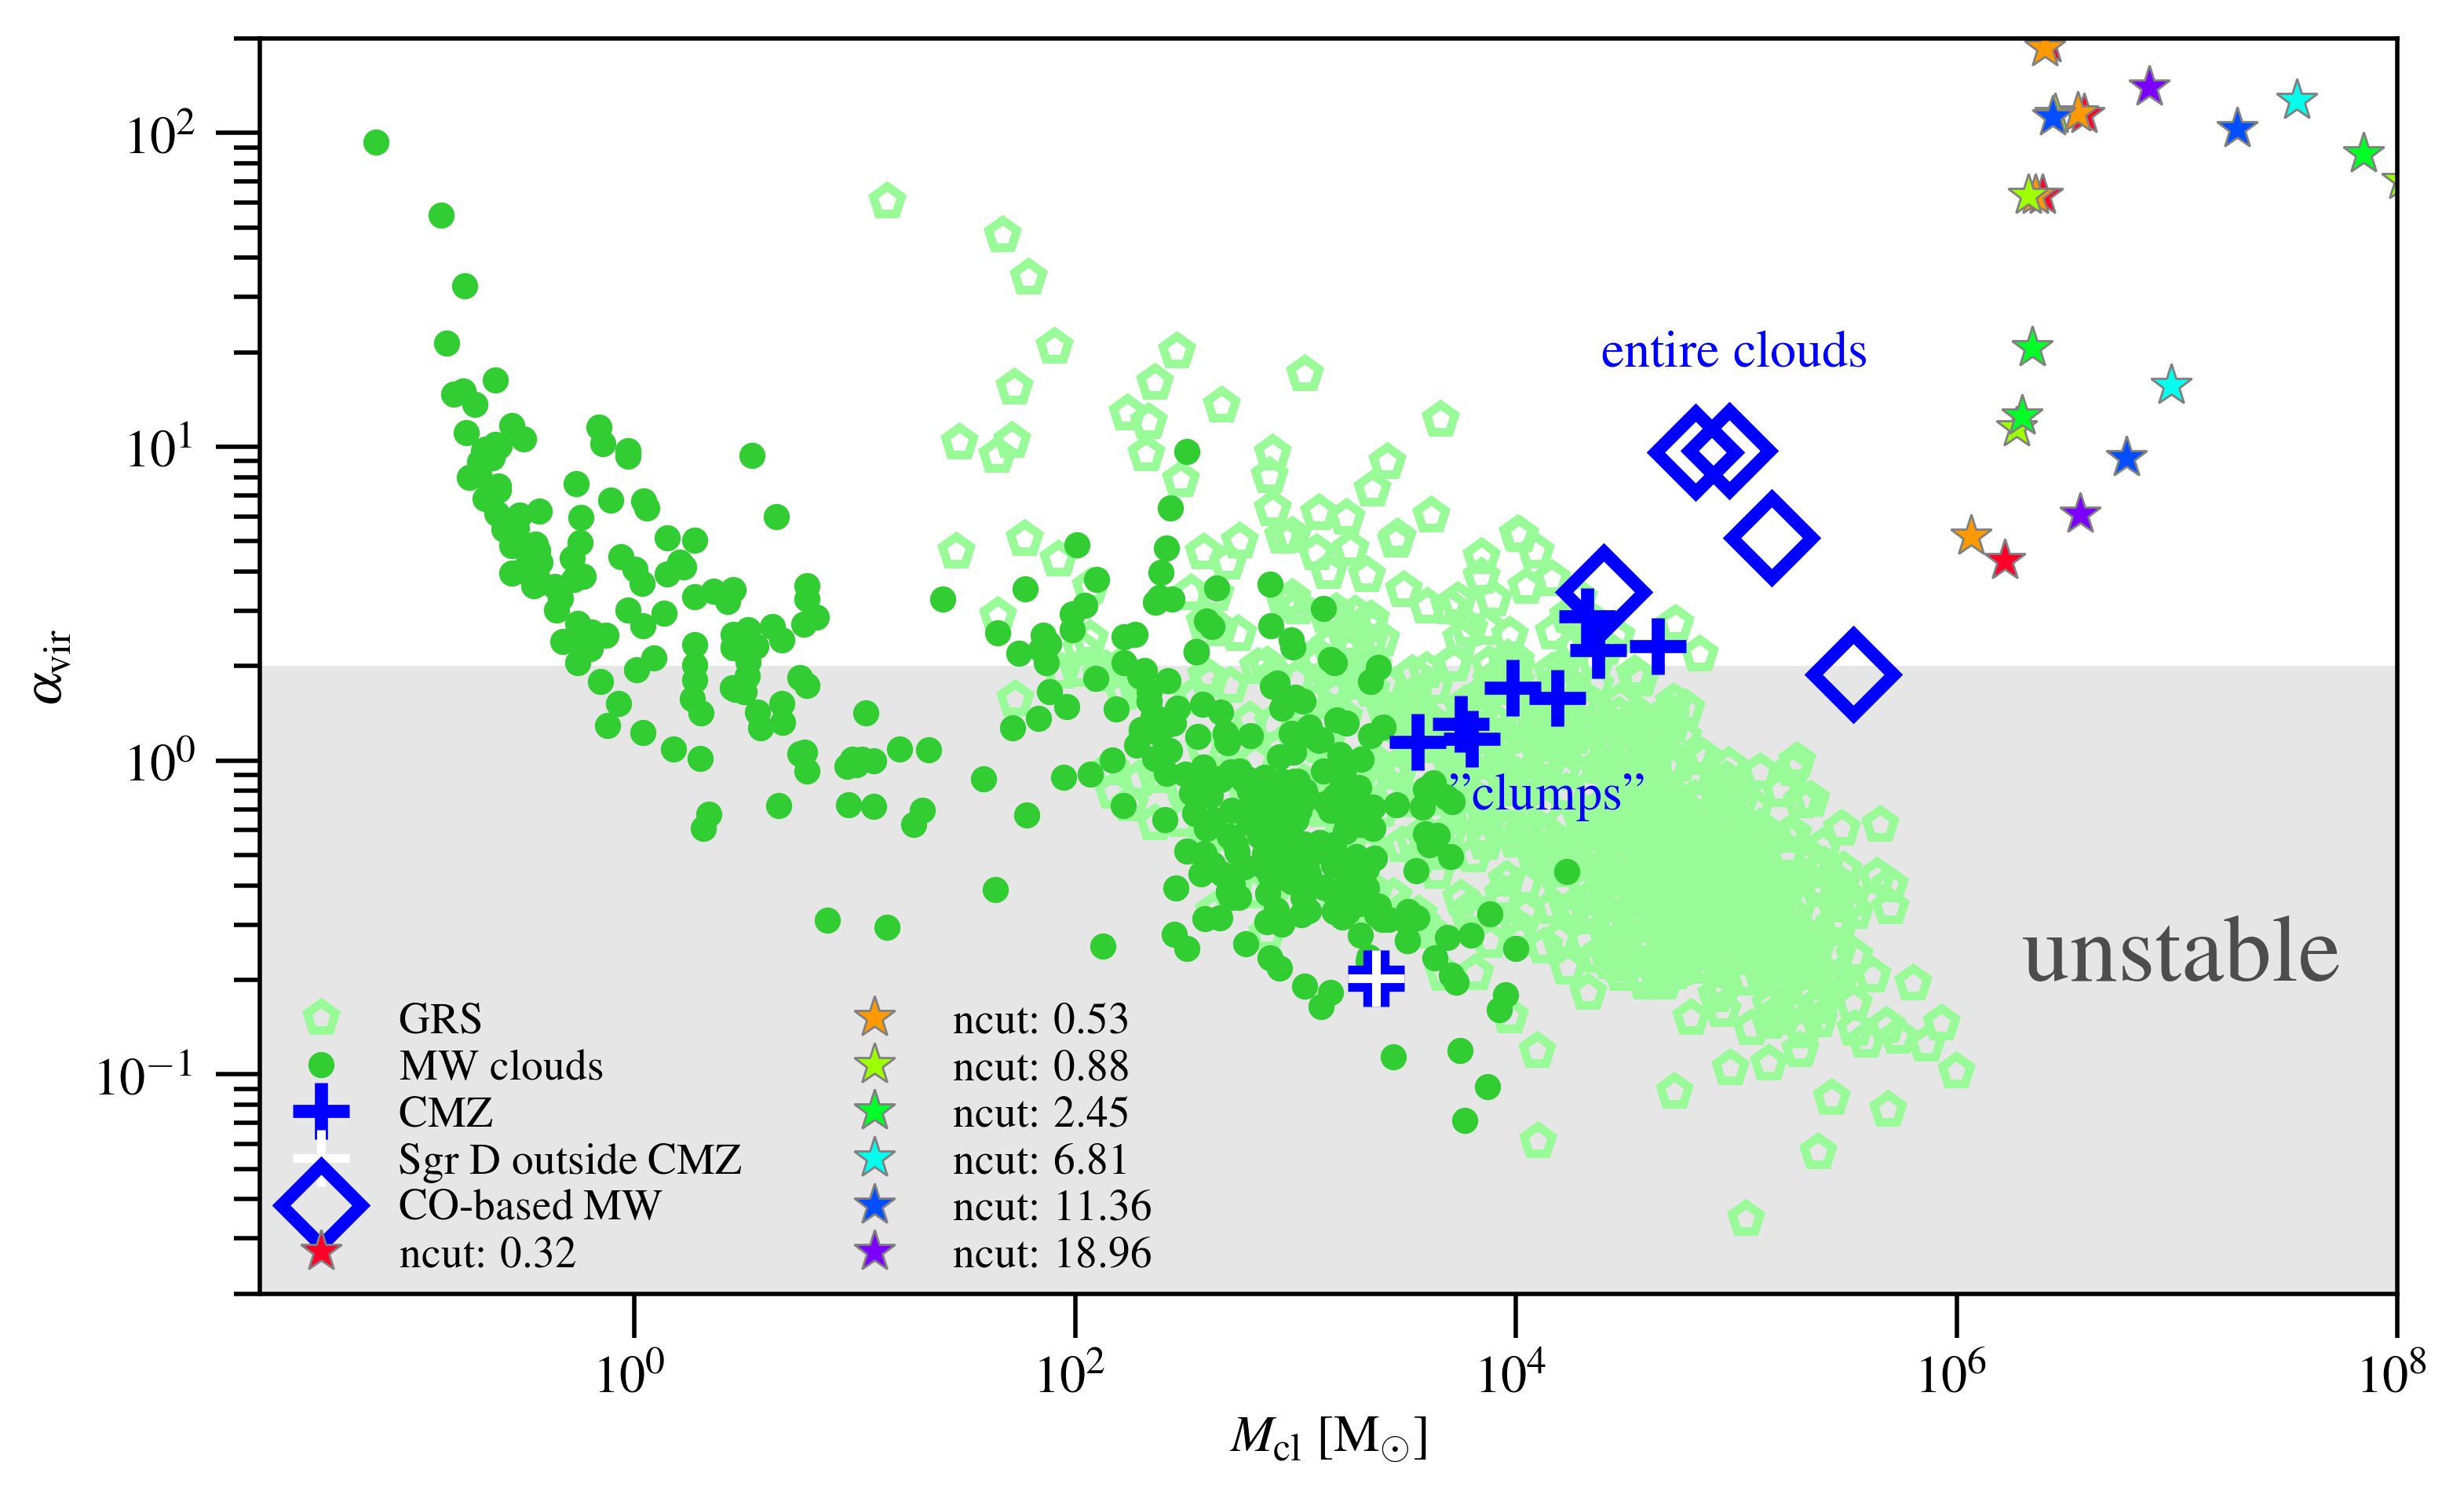
\includegraphics[trim=0 0 0 0, clip, width=0.85\textwidth]{\figpath/ss27_alphavir.png}
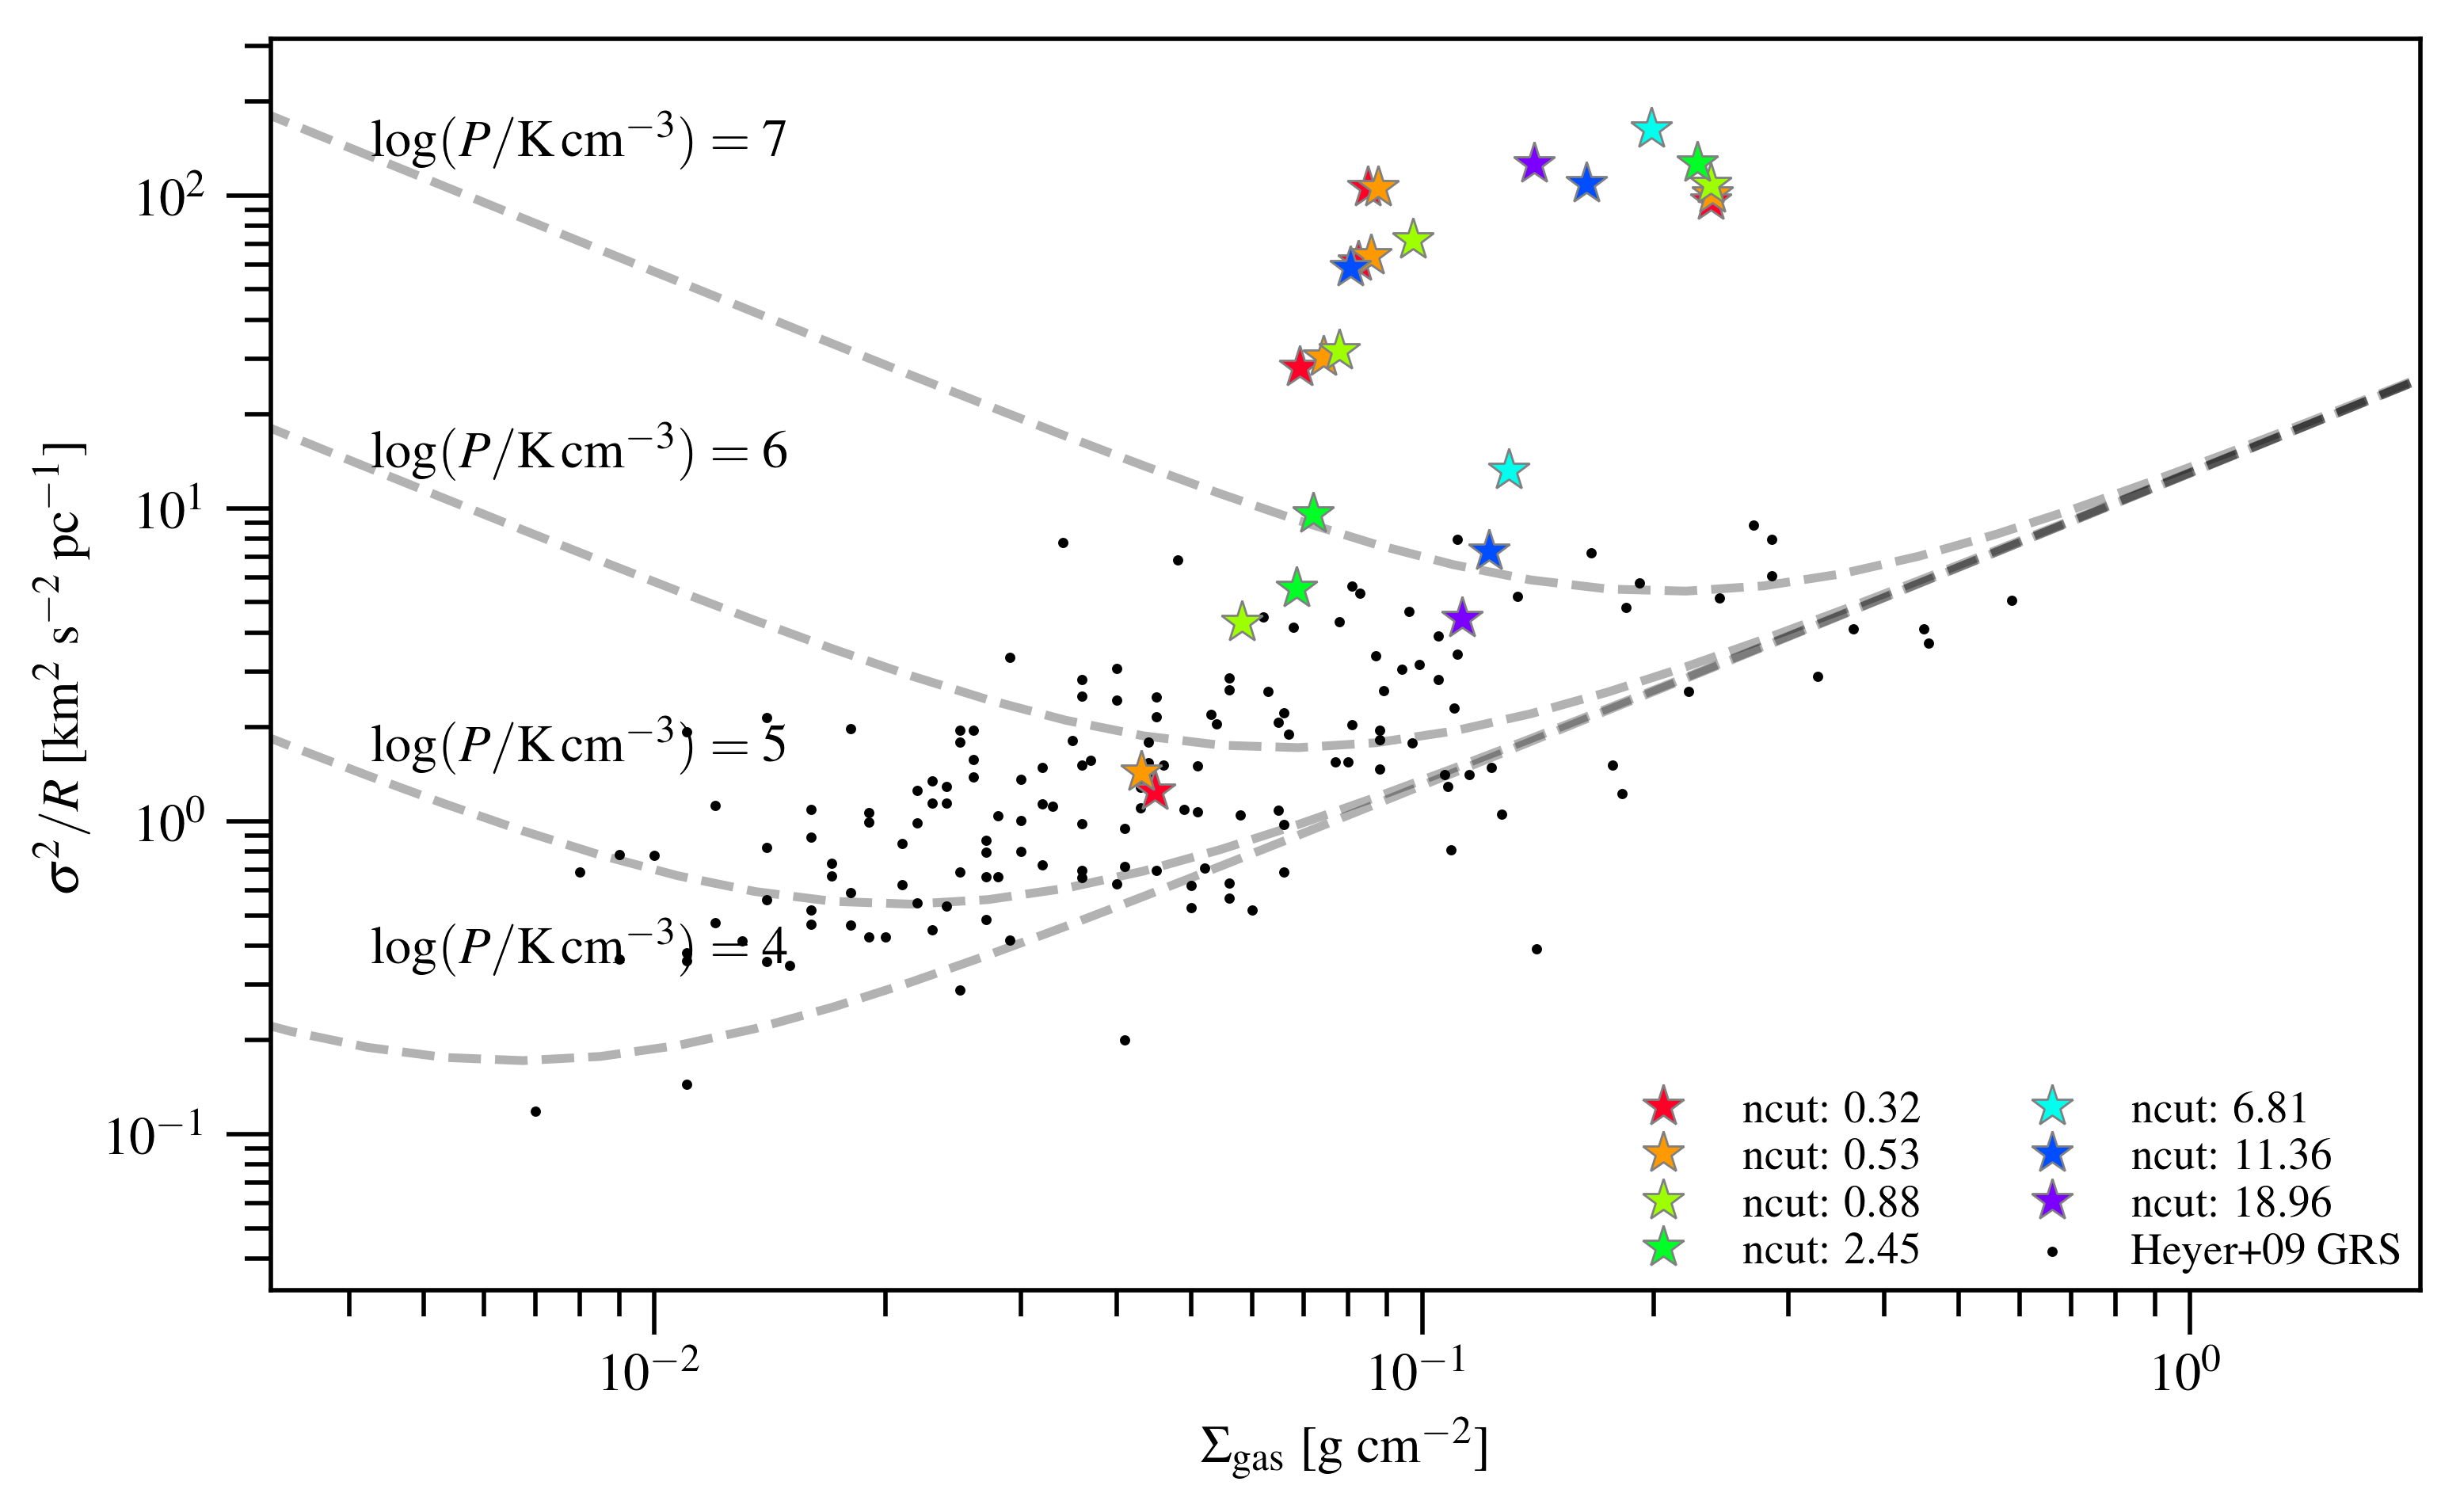
\includegraphics[trim=0 0 0 0, clip, width=0.85\textwidth]{\figpath/ss27_PVE.png}
\caption{
Top: Virial parameter and cloud mass of \flower of a given snapshot (starburst phase).
Bottom: $\sigma^2/R - \Sigma_{\rm gas}$ relation of MCs in the same snapshot.
\label{fig:alpha27}}
\end{figure*}




% -------------- all snapshots -----------


\begin{figure*}[htbp]
\centering
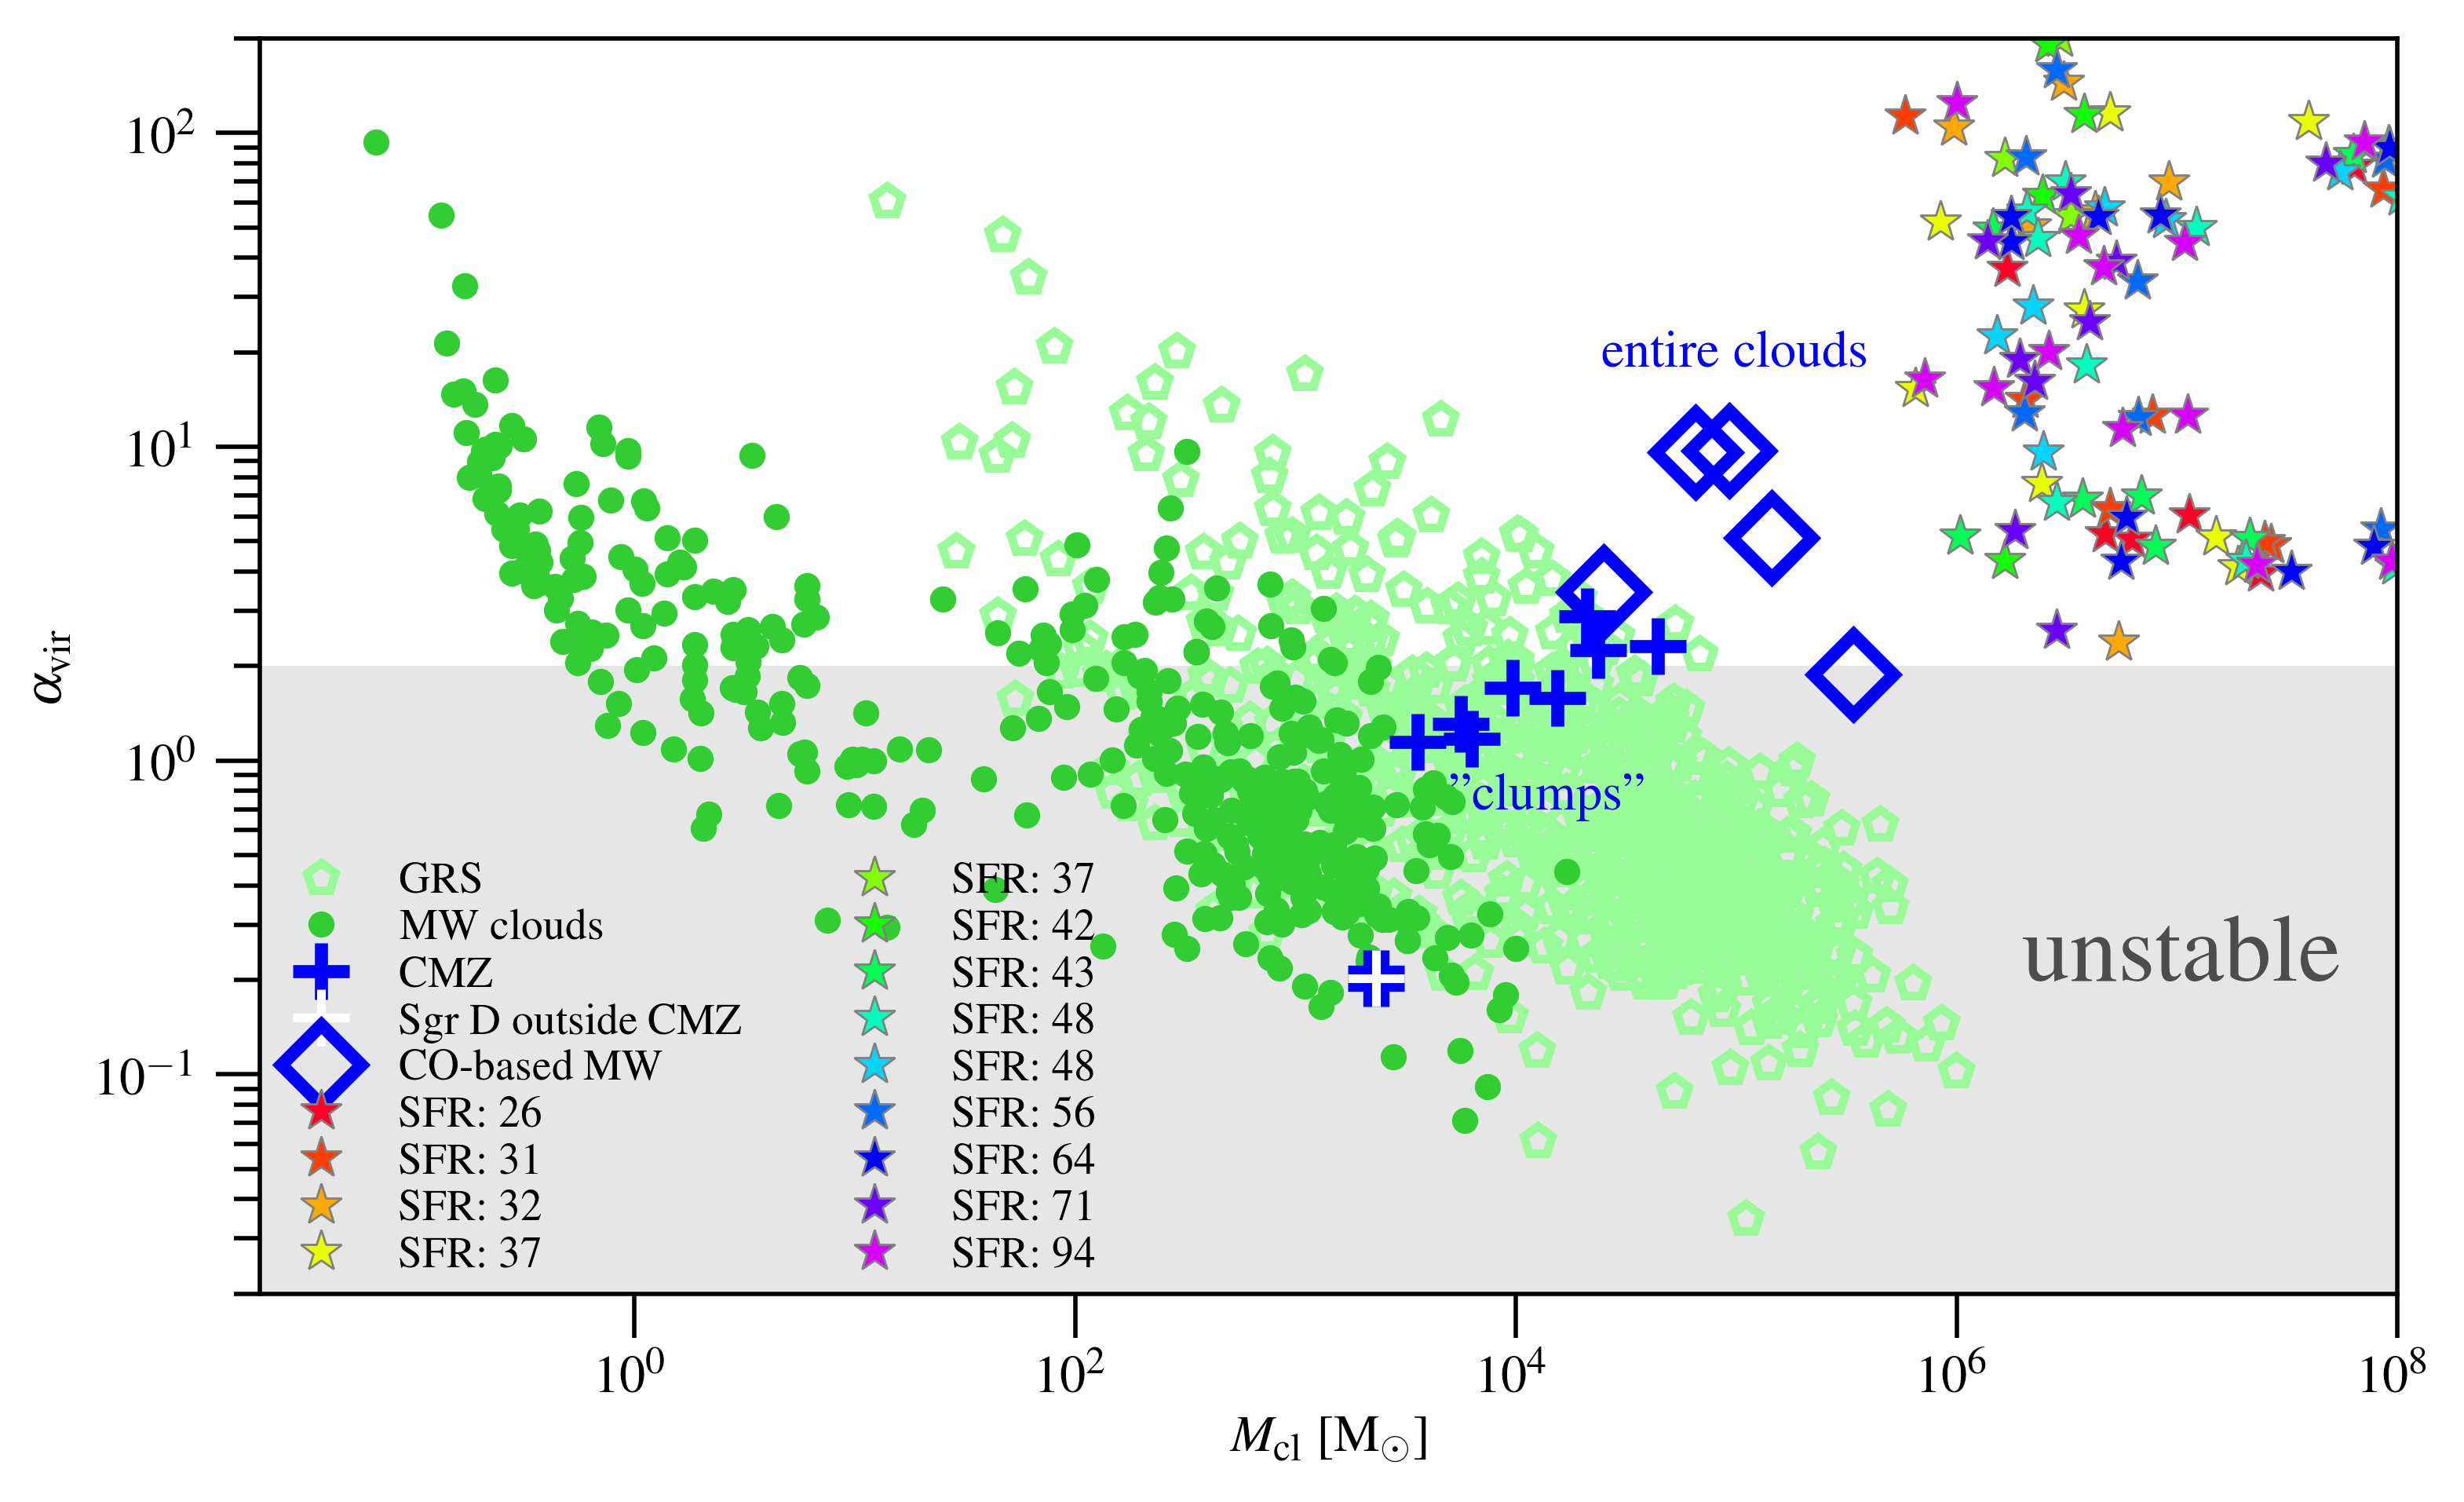
\includegraphics[trim=0 0 0 0, clip, width=0.85\textwidth]{\figpath/ss16-28_alphavir.png}
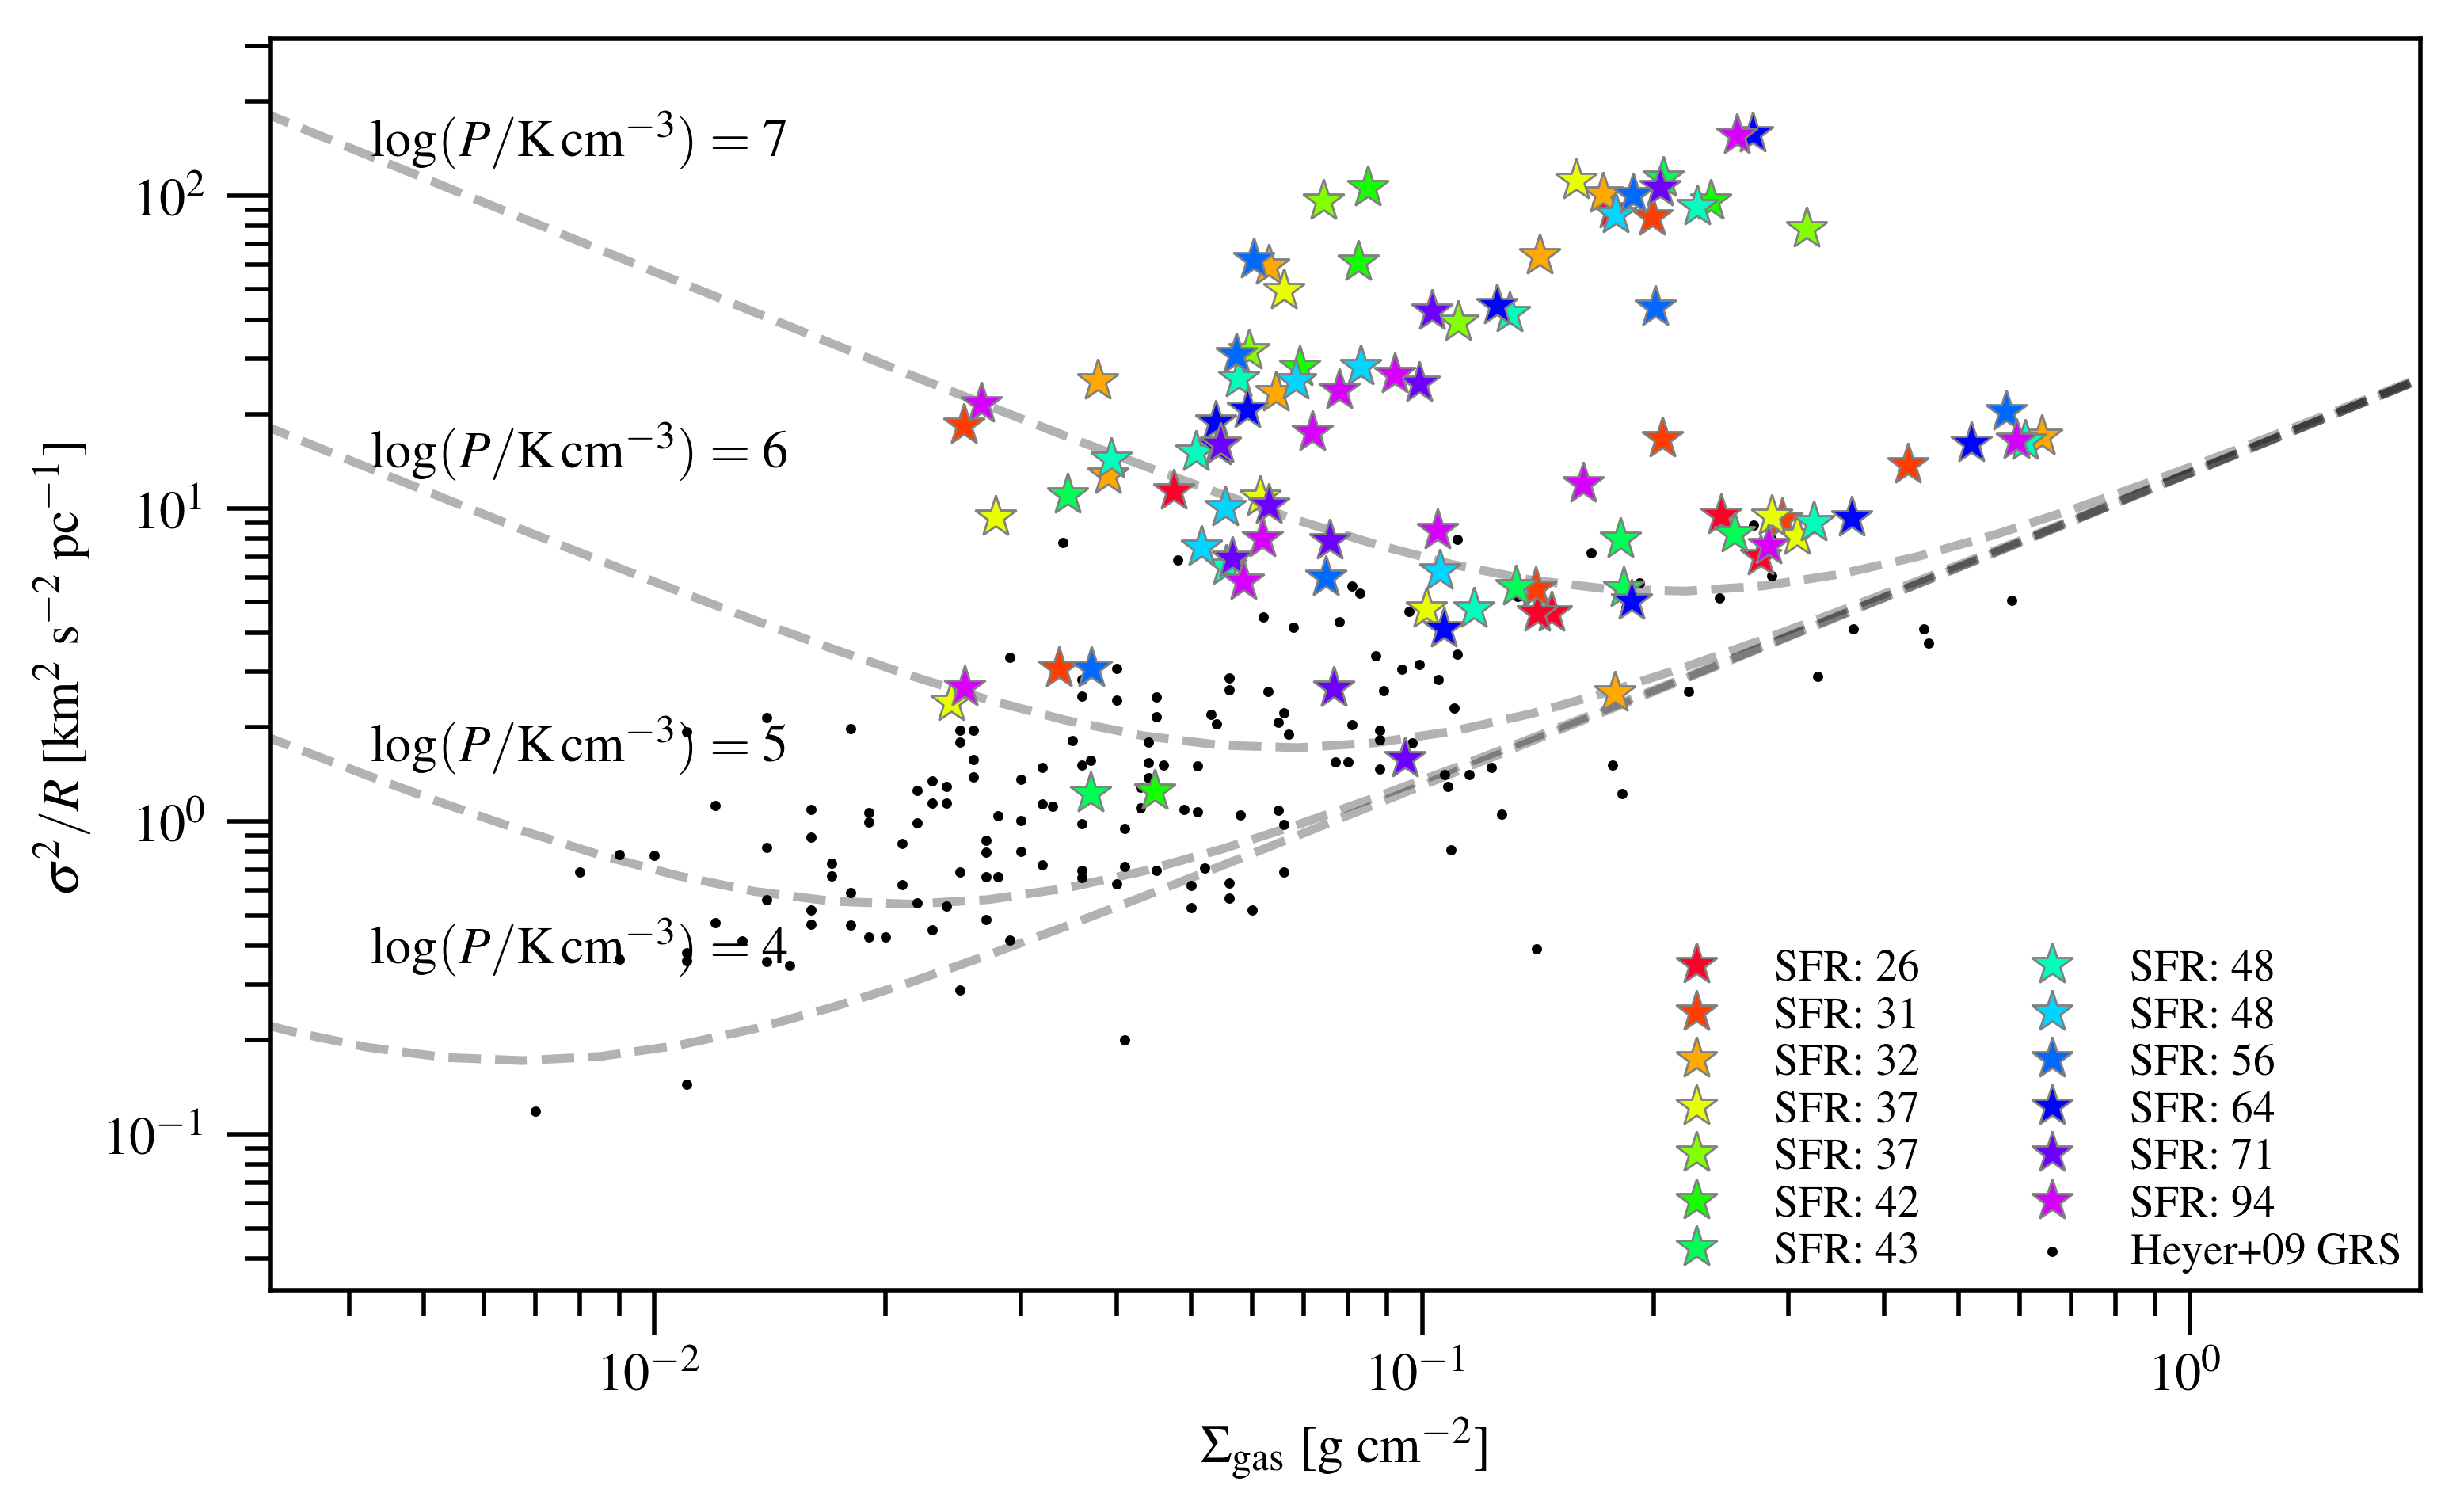
\includegraphics[trim=0 0 0 0, clip, width=0.85\textwidth]{\figpath/ss16-28_PVE.png}
\caption{
Top: Virial parameter and cloud mass of MCs in \flower identified across all snapshots.
Bottom: $\sigma^2/R - \Sigma_{\rm gas}$ relation of MCs.
\label{fig:alpha16-28}}
\end{figure*}

\begin{figure*}[htbp]
\centering
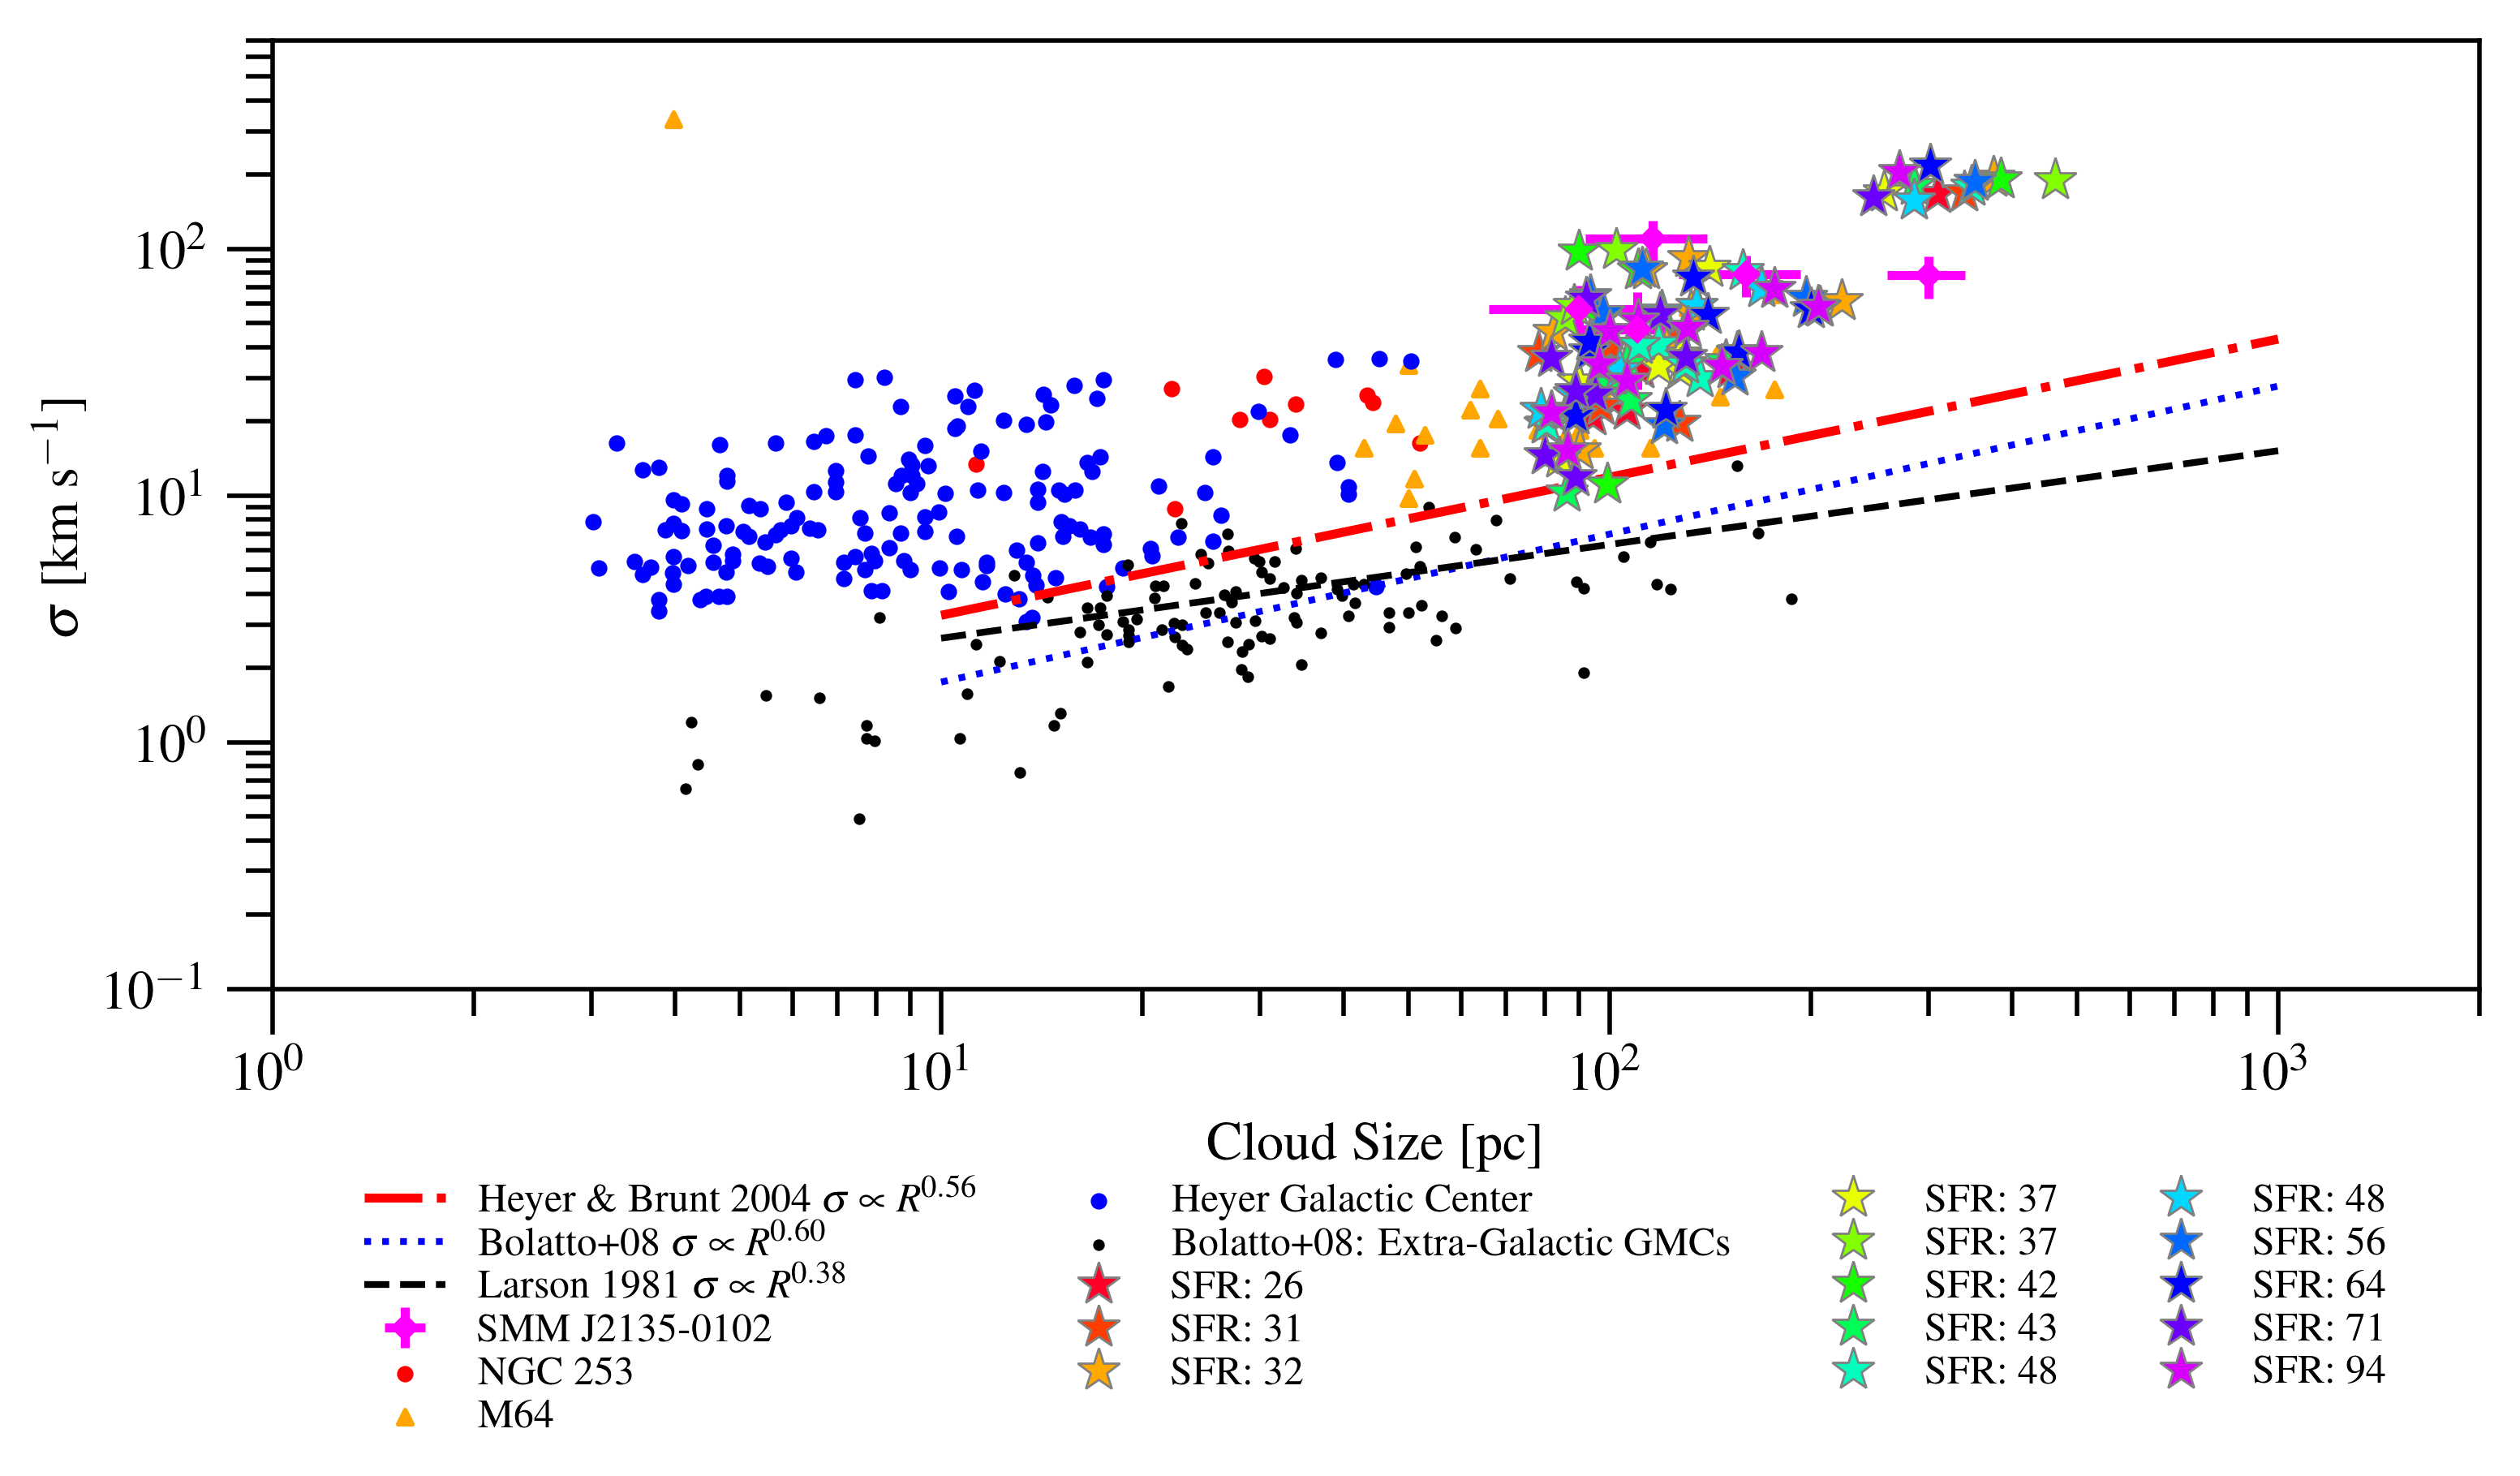
\includegraphics[trim=0 0 0 0, clip, width=0.85\textwidth]{\figpath/ss16-28_larsons.png}
\caption{
Larson's relation of \flower across all snapshots (showing MC properties in different evolutionary
phases) and
those observed in nearby and the \z$\sim$2 star-forming galaxy.
\label{fig:larsons16-28}}
\end{figure*}


\begin{figure*}[htbp]
\centering
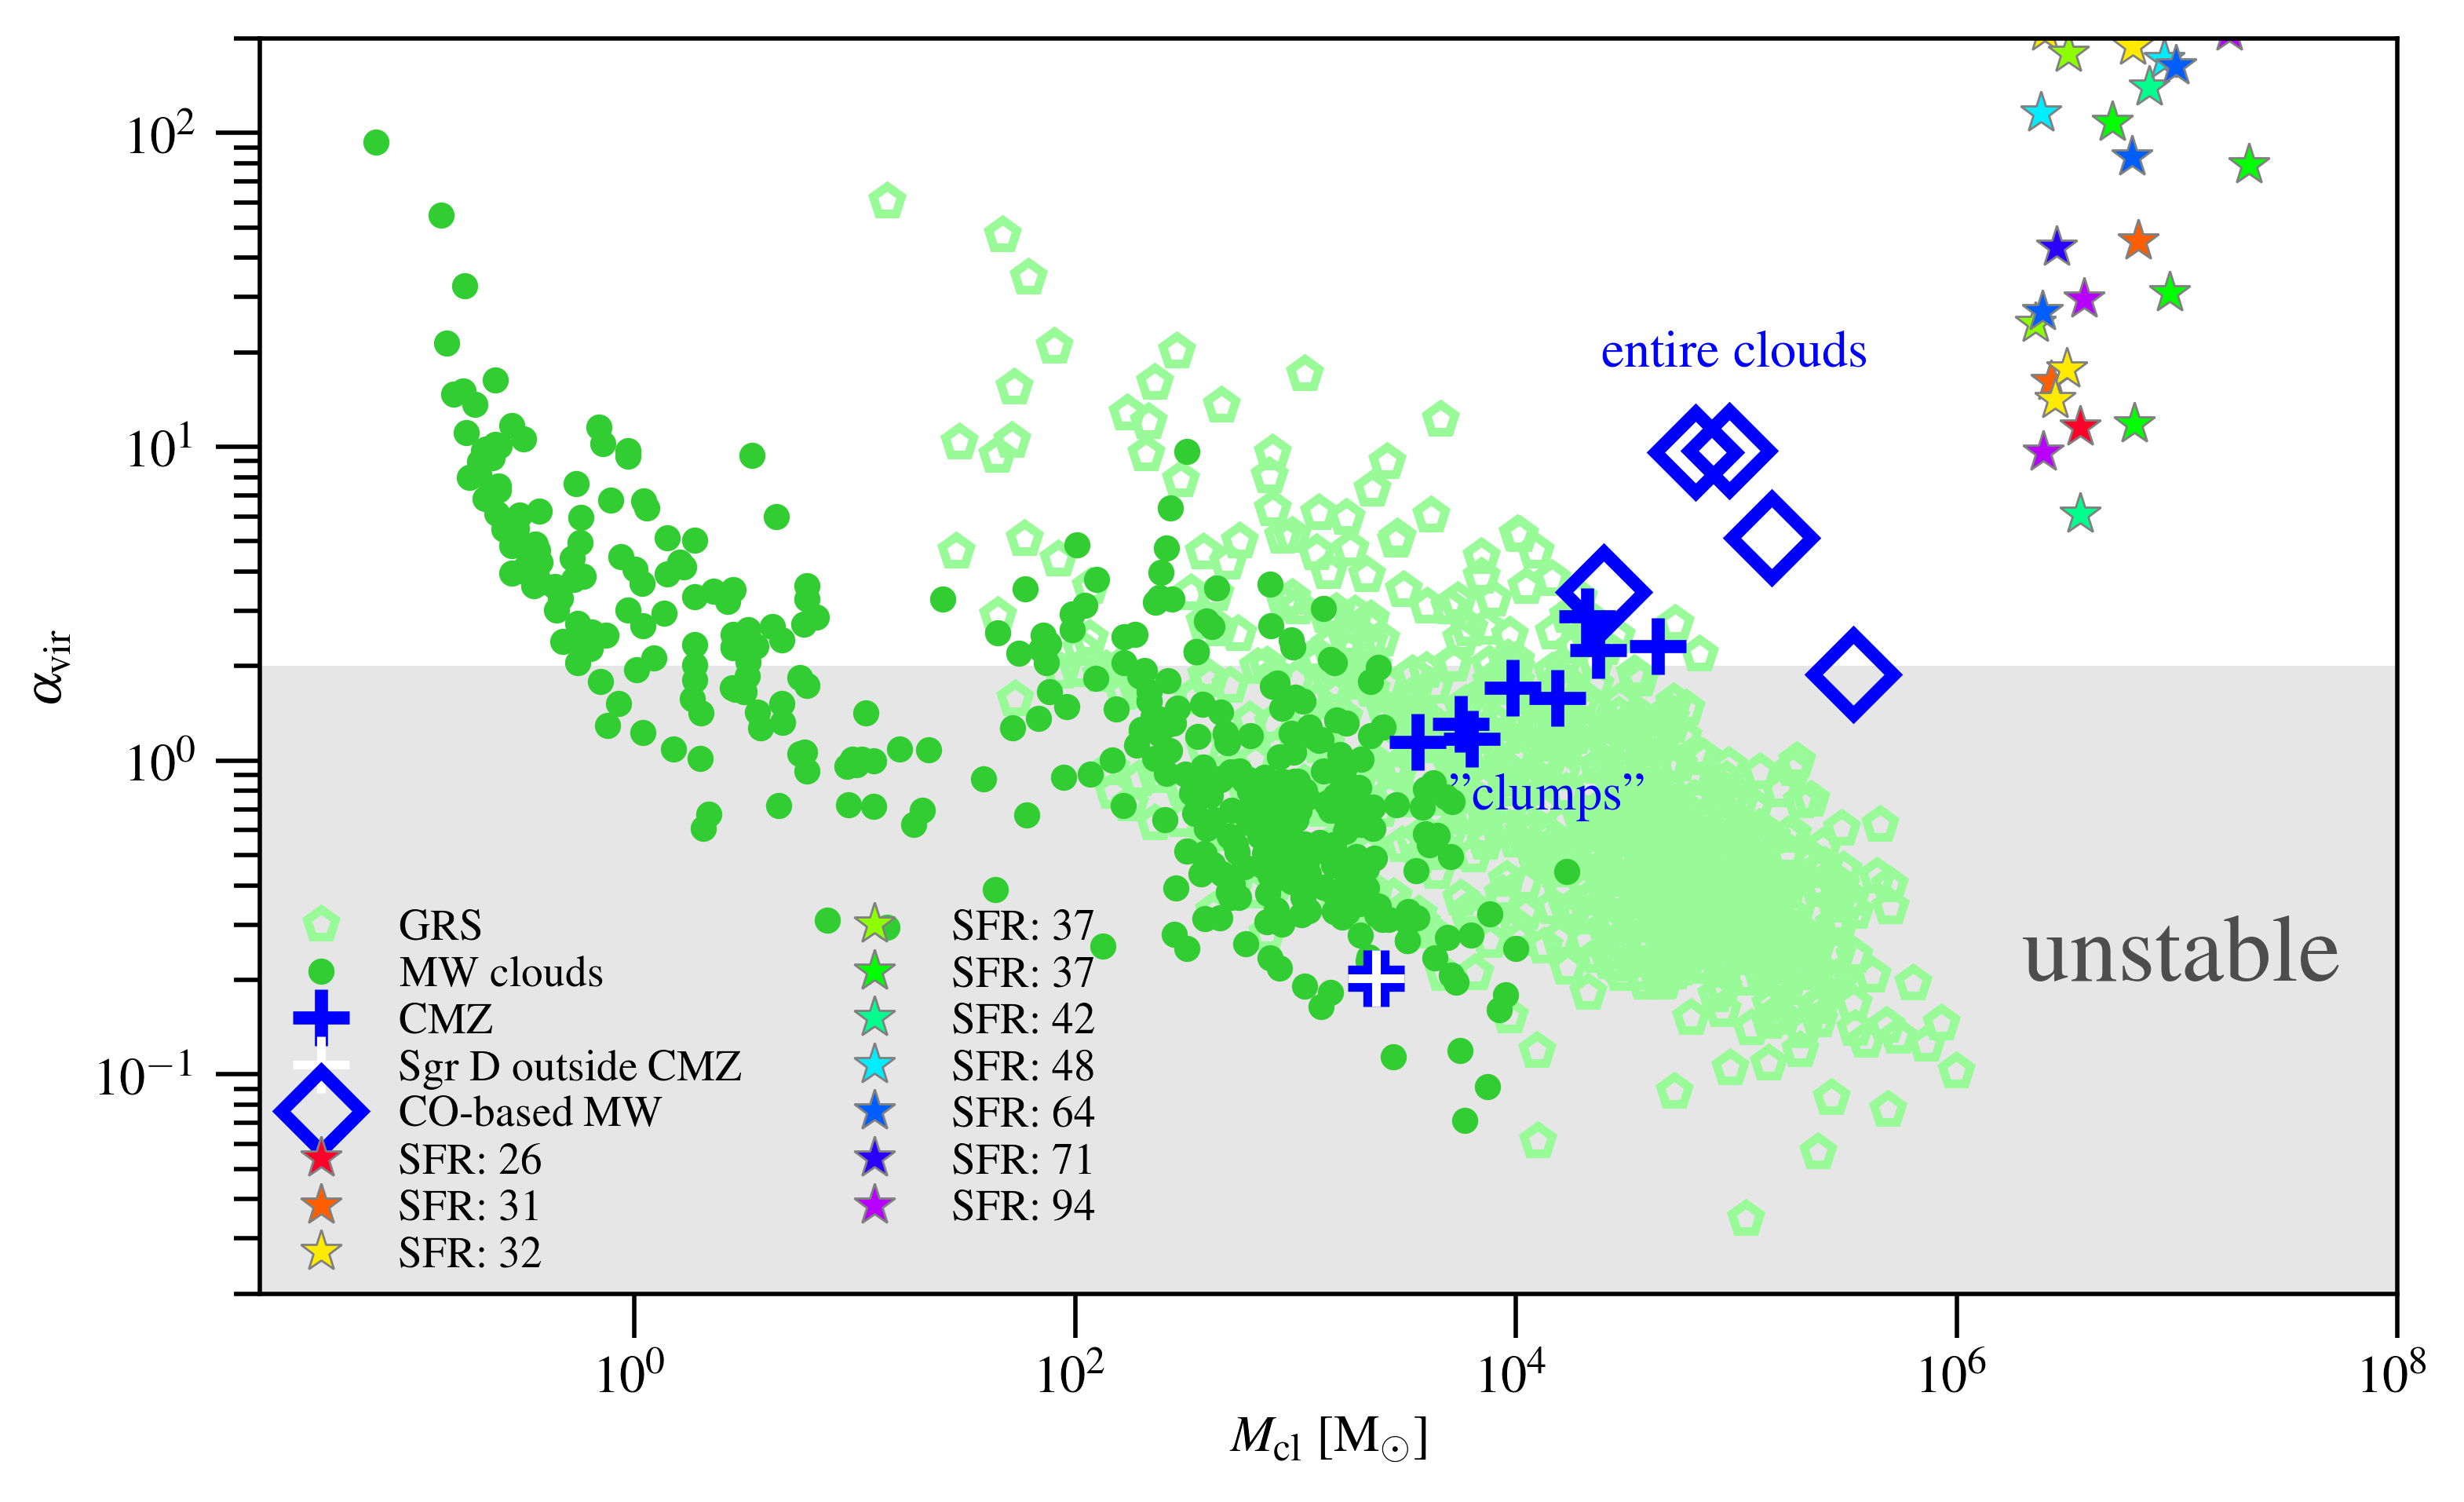
\includegraphics[trim=0 0 0 0, clip, width=0.85\textwidth]{\figpath/ss16-28-alphavir-highncut.png}
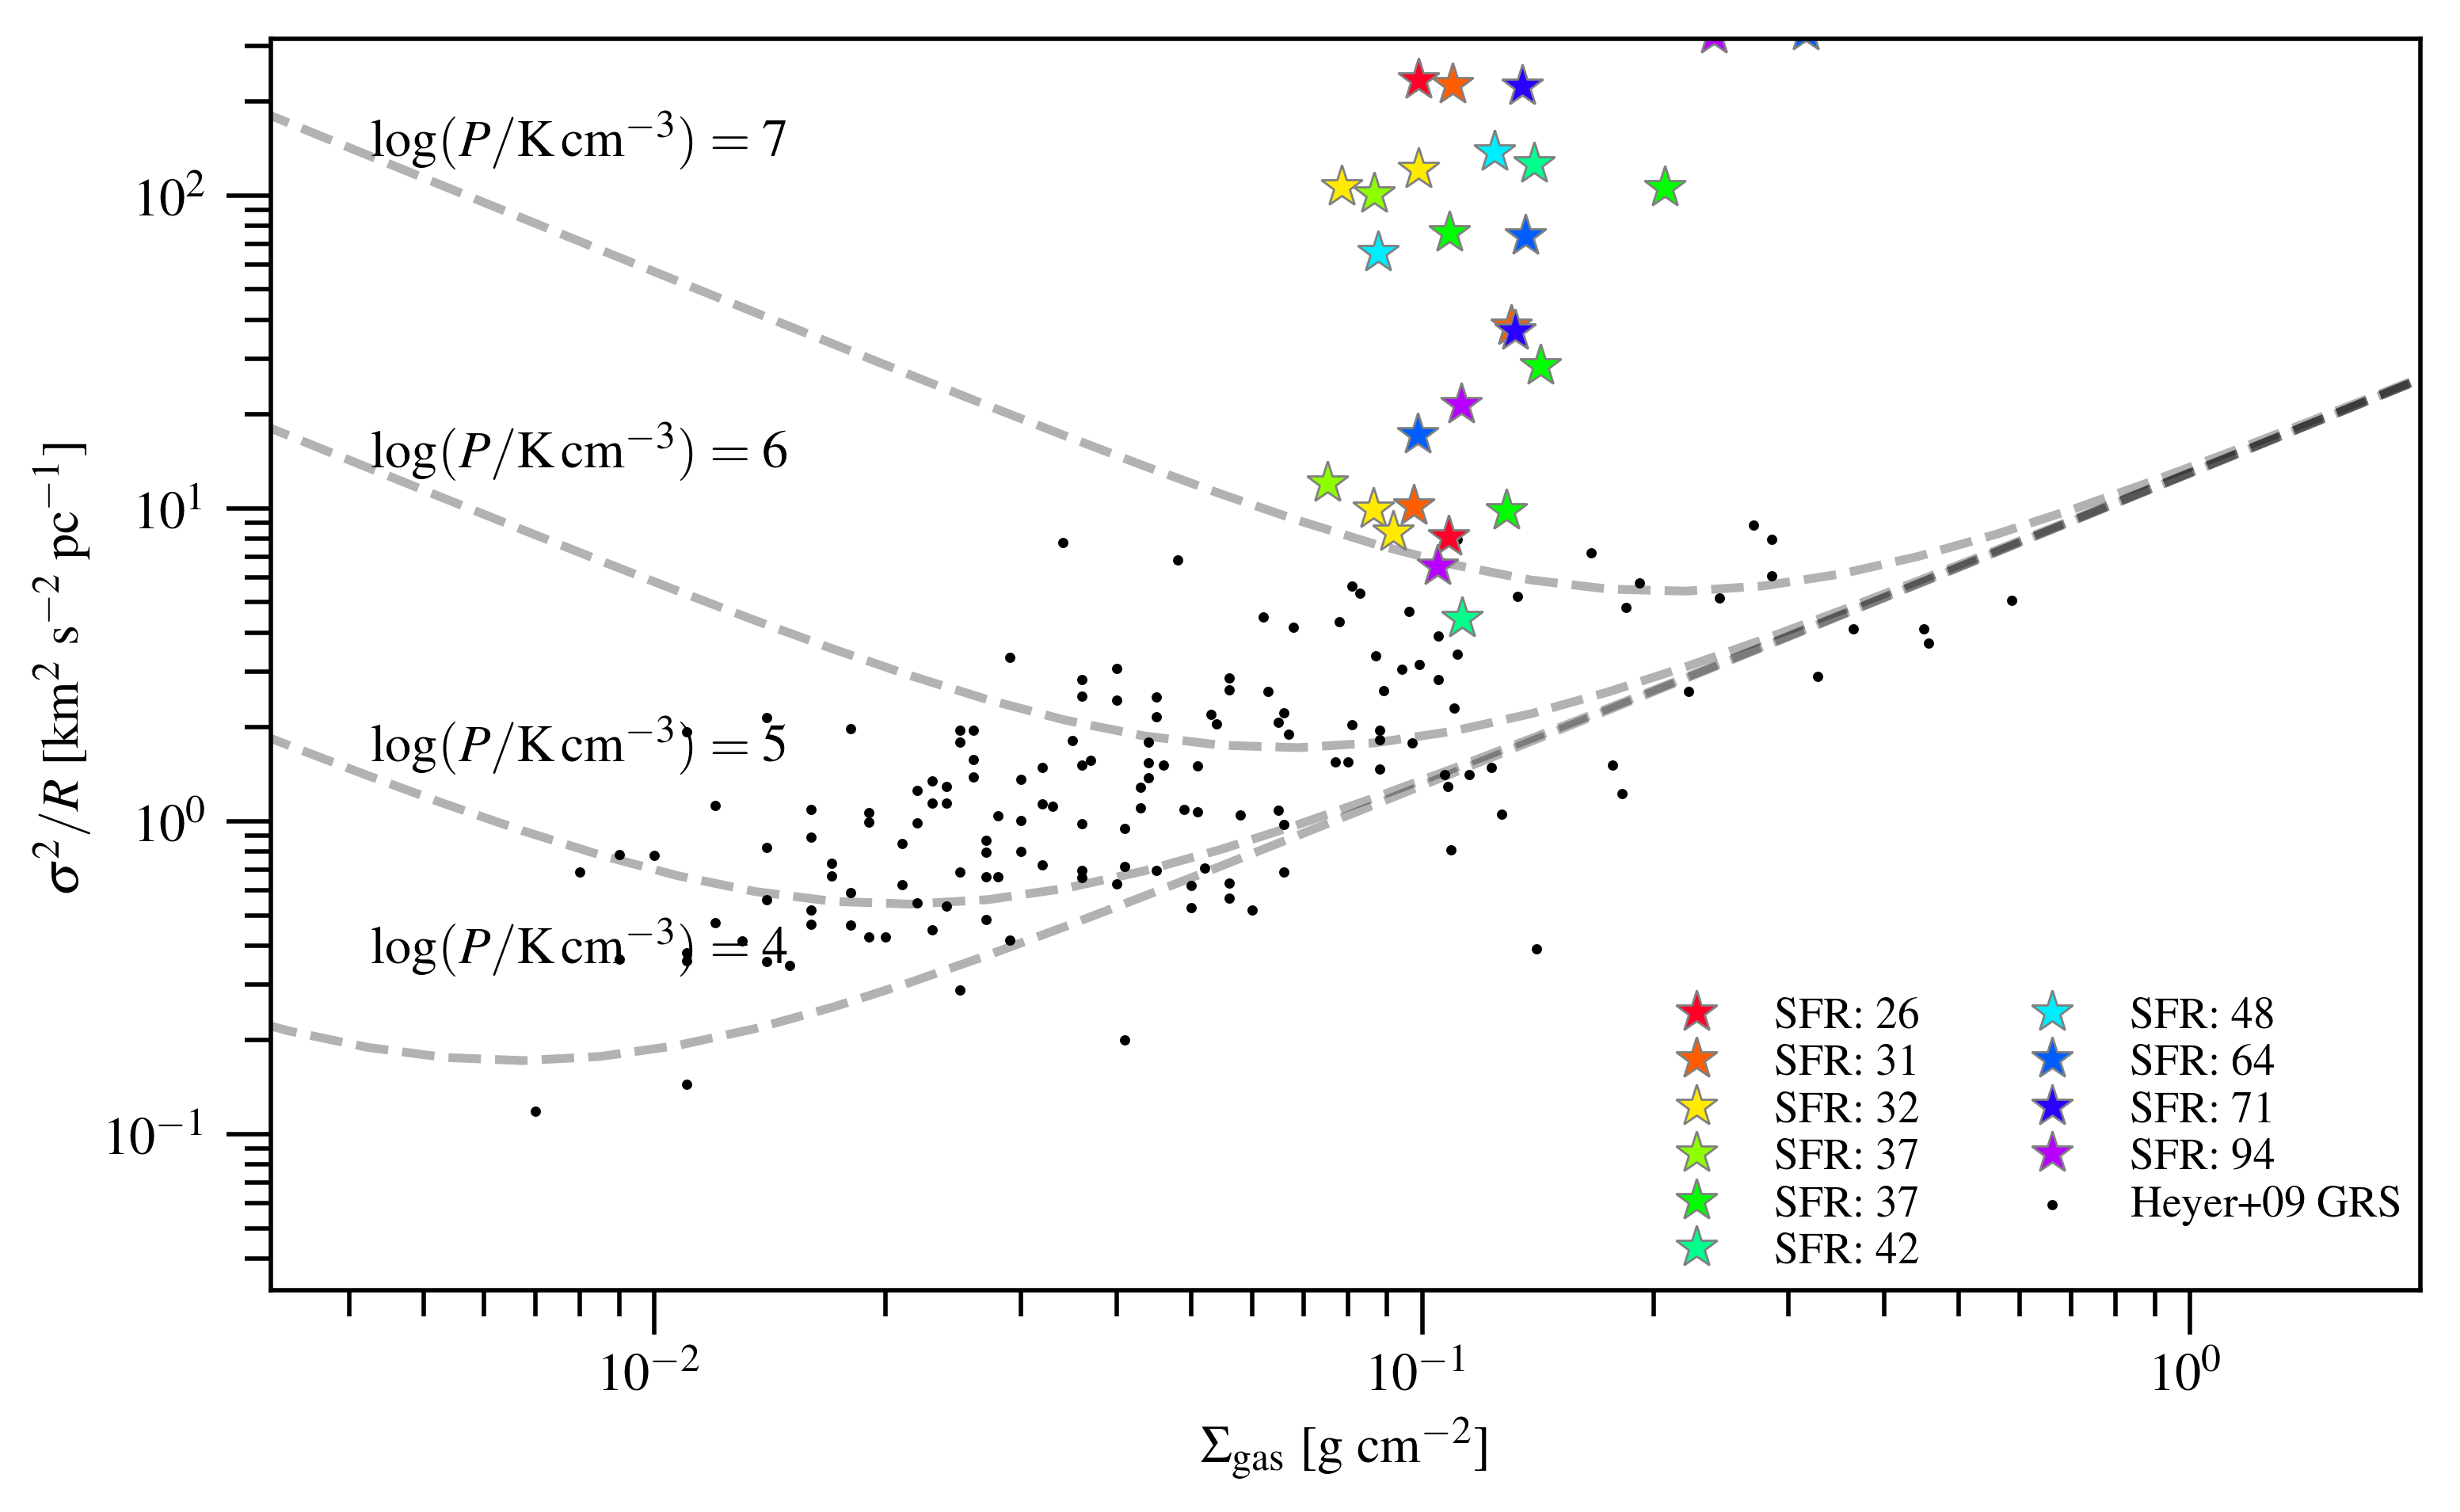
\includegraphics[trim=0 0 0 0, clip, width=0.85\textwidth]{\figpath/ss16-28-PVE-highncut.png}
\caption{
Same as \Fig{alpha16-28}, but MCs here are those identified from the highest $n_{\rm cut}$,
where only denser substructures of the main disk of \flower are included.
\label{fig:alpha16-28-highncut}}
\end{figure*}

\begin{figure*}[htbp]
\centering
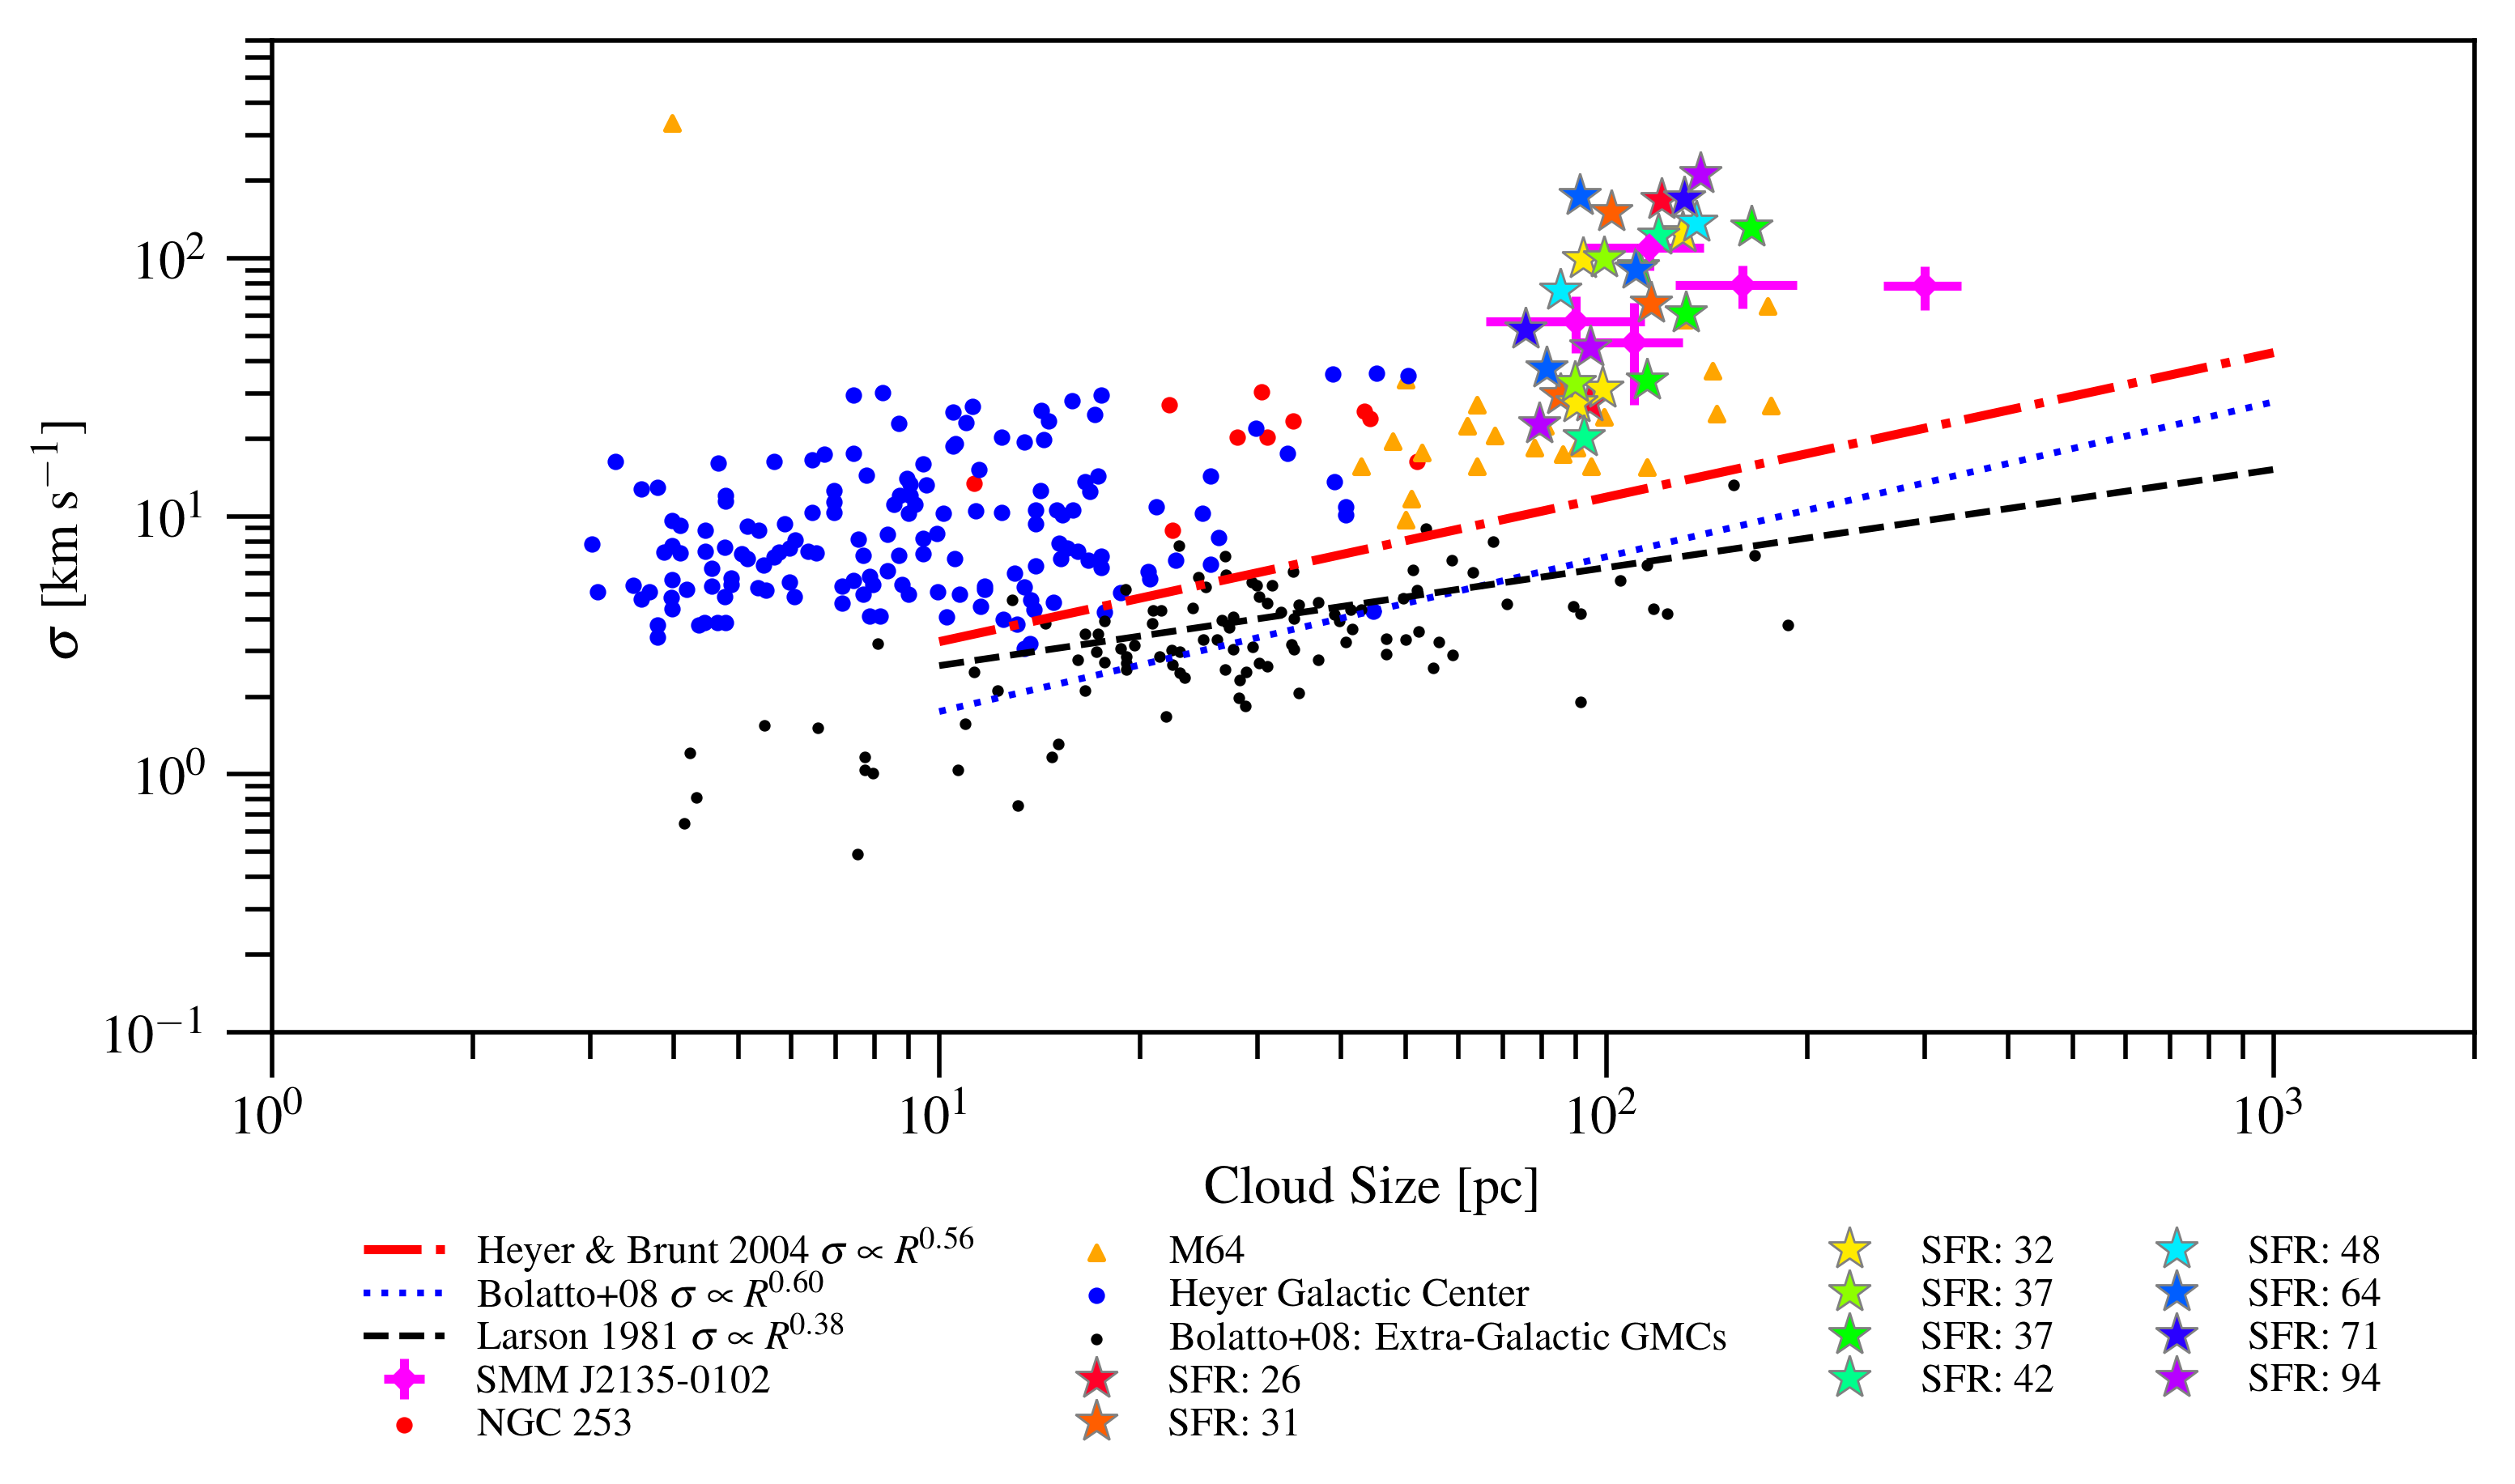
\includegraphics[trim=0 0 0 0, clip, width=0.85\textwidth]{\figpath/ss16-28-larsons-highncut.png}
\caption{
Same as \Fig{larsons16-28}, but MCs here are those identified from the highest $n_{\rm cut}$,
where only denser substructures of the main disk of \flower are included.
\label{fig:larsons16-28-highncut}}
\end{figure*}

% cloud structures at large and small scale
% Larson's: m = 460 M_sun (r_pc)^1.9 for structure w/in molecular clouds. --> $m \propto r^2$ \citep{McKee07a} (law of constant
% column density) as fundamental properties of molecular cloud structure.
Larson's third relation describes fundamental properties of molecular clouds, relating their structures on small and large scales 
via two physical properties: mass and size \citep{Larson81a, Mckee07a}. This is also known as the law of constant column density, 
since cloud mass in \obs is sometimes derived by integrating
over the mass surface density ($\Sigma$), which is related to the column density ($N_{\rm H2}$) obtainable from extinction maps ($A_V$).   
That is, $N_{\rm H2}\propto A_V$, $\Sigma\propto N_{\rm H2}$, and $M$\eq$\int \Sigma~dA$.
Therefore, cloud mass is related to $N_{\rm H2}$ and $A_V$.

We show in \Fig{MR} the size-mass relation of the MCs of \flower in the accreting phase (see \Sec{sfh})
compared to the empirical relation obtained based on 
Milky Way data (\citealt{Kauffmann10b, Kauffmann10c} and references therein),
which we extrapolate to match the mass and size scales of the MCs of \flower.
By comparing the masses and sizes found in clouds without massive \SF ($<$10\,\Msun) 
in the solar neighborhood ($\lesssim 500$\,pc; Taurus, Perseus, Ophiuchus, and the 
Pipe Nebula) with those with massive \SF in the Milky Way, \citet{Kauffmann10c} report a 
mass-size relation of $M \gtrsim 870$\,\Msun$\times\,\left(r/{\rm pc}\right)^{1.33}$ as the threshold for massive \SF. 
That is, cluster-forming cloud fragments are found to be more massive than those that are devoid of clusters 
at a given radius. As shown in \Fig{MR}, the MCs identified in the accreting phase of \flower lie above this relation, along to the locus 
with visual extinction of $A_V$\eq4\,mag. {\bf This may suggest ....}
We also examine the size-mass relation of the MCs identified in other snapshots, finding that they lie in the same 
parameter space as the accreting phase.

\begin{figure*}[htbp]
\centering
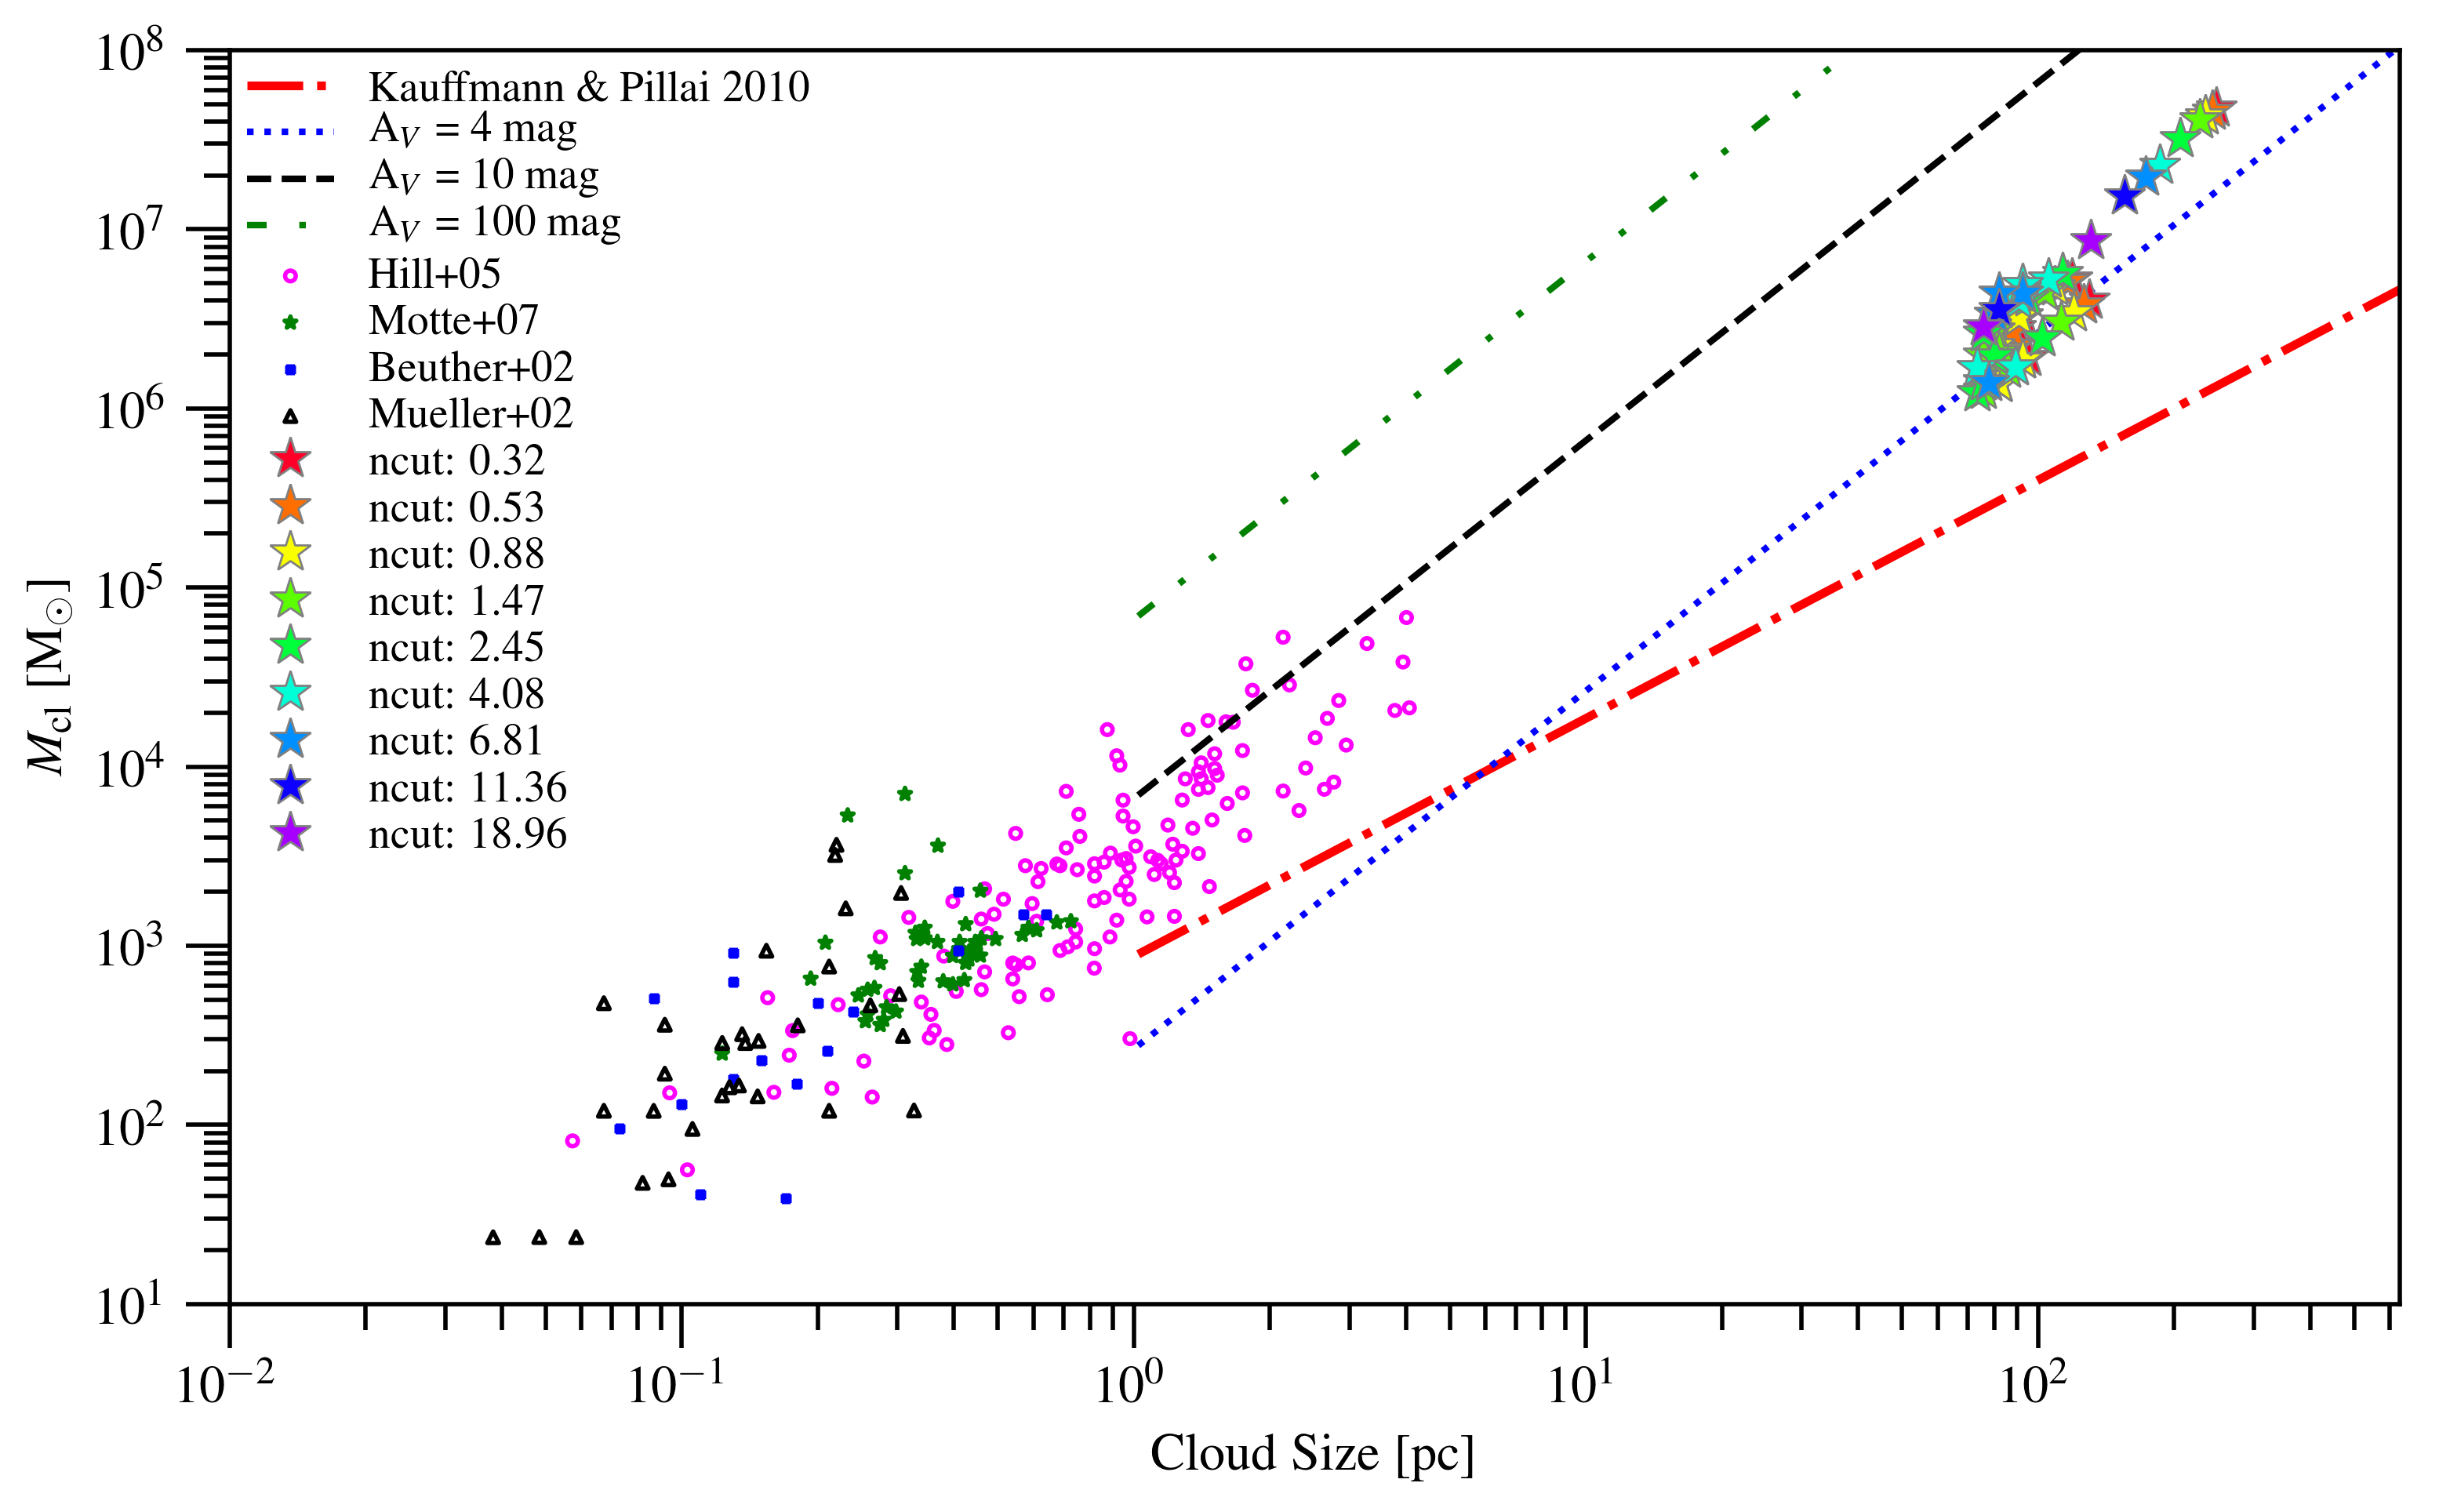
\includegraphics[trim=0 0 0 0, clip, width=0.85\textwidth]{\figpath/lf16_cloud-mass_size-pc.png}
\caption{
Size-mass relation of MCs in \flower compared to data and empirical established based on Milky Way \obs.
Star symbols show MCs identified in the accreting phase of \flower in our simulation, color-coded by increasing $n_{\rm cut}$.
Other symbols show the masses and sizes of molecular clouds with massive \SF observed in the 
Milky Way \citep{Beuther02a, Mueller02a, Hill05a, Motte07a}.
Red line shows the threshold for massive \SF reported by \citet{Kauffmann10b}.
\label{fig:MR}}
\end{figure*}


%\subsubsection{Single Snapshots: SFR-Mach-$\alpha_{\rm vir}$ Relation}
%%M~ 30 in normal spirals \citep{McKee99a}
%%M~ 100 in SBs \citep{Downes98a}
%In the following, SFR of each MC is calculated by integrating over the recent \SF history of stars within each MC. 
%More specifically, we sum up all the stellar masses with stellar age of $<$10\,Myr and  normalized 
%the mass over this period of time.
%In \Fig{}, we show the relation between SFR and the Mach number ($\mathcal{M}$) for the molecular
%complexes identified.
%We find a positive correlation between the two quantities, with a Pearson-$R$ coefficient of xxx,
%which is unsurprising given that our simulations include the effect of stellar feedback. That is,
%the high $\mathcal{M}$ can be interpreted as a result of \SF resulting from feedback from
%massive stars.



\subsubsection{Variation in MC Properties Depending on the Choice of Density Cuts}	 \label{sec:ncut}
% single Snapshot
We investigate possible variations in the dynamics of the molecular structures of \flower and its satellites
to test
the robustness of our results against the choice of density threshold by adopting
different sets of $n_{\rm cut}$ in identifying the MCs.
That is, how sensitive are the structure properties, and thus, the results presented in \Sec{singless}
dependent on the choice of density thresholds.
We vary the choice of H$_2$ density for each of the snapshots and
find no obvious differences in our results (i.e., inferences on the dynamics of \z$\sim$\,6
MCs in relation to those observed in nearby and \z$\sim$2 galaxies in the context of
cloud scaling relations).
In addition, for the densest MC in the main disk of \flower, we find that while
its cloud size decreases as we increase $n_{\rm cut}$ --- as one would intuitively expect,
its velocity dispersion remain
approximately $\sigma\simeq$200\,\kms (\Fig{larsons_single}).
This lack of variation is reassuring, in the sense that at least on the scales studied here,
the dynamics of the MCs are not artifacts or biased by our choice of $n_{\rm cut}$.
Our results is therefore robust, haha.

%\begin{figure*}[tbph]
% \centering
%\includegraphics[width=\textwidth]{\figpath/.pdf}
%\caption{\label{fig:}}
%\end{figure*}




\section{Origin of the clumps: Mass Scales set by Toomre and Jeans Instabilities}   \label{sec:Q}
The onset of gravitational instability is considered to be tightly connected to (the conditions for) \SF \citep[e.g.,][]{Kennicutt89a, Li05b, Li06a}
and is widely discussed in the context of the Toomre stability criterion \citep{Toomre64a, Goldreich65b}.
For axisymmetric mode ($m$\eq0), the dispersion relation for the growth of density perturbation in a rotating turbulent disk
of finite thickness $h$
is described by:
\begin{equation}
\omega^2 = \kappa^2 - \frac{2\pi G \Sigma |k|}{1 + |k| h} + \sigma^2 k^2,
\label{eqn:3Ddisp}
\end{equation}
where $k$ is the wavenumber in the disk and $\kappa$ is the epicyclic frequency.
The first term on the RHS describes rotation support, second term describes self-gravity, and
the third term describes pressure support.
The epicyclic frequency is defined as:
\begin{equation}
\kappa^2\equiv\frac{2\Omega}{R}\frac{d}{dR}\left(R^2\Omega\right).
\label{eqn:kappa}
\end{equation}
% \kappa\propto\Omega
One can then define the so-called Toomre-Q parameter/criterion for stability as
\begin{equation}
Q\equiv\frac{\sigma\kappa}{\pi G \Sigma}.
\label{eqn:Q}
\end{equation}
We can then rewrite Equation~\ref{eqn:3Ddisp} in terms of
\begin{equation}
\omega^2 = Q^2 k^2 \left(\frac{\pi G \Sigma}{\kappa}\right)^2 - 2\pi G \Sigma |k| + \kappa^2.
\end{equation}
Thus, for $Q\lesssim$1, disk is unstable for some $k$ ($\omega^2 < 0$)
and fragmentation can happen
(e.g., instability impose by angular momentum from gas accretion from the cosmic web and
satellite galaxies and stellar feedback).
That is, local fragmentation takes place when gravity overcomes pressure support
from turbulence (thermal is small here) and shearing of differential rotation.

In the limit of a thin rotating disk, rotation can help stabilizes
self-gravitational contraction for wavelengths greater than the Toomre length:
\begin{equation}
\lambda_T = 4\pi^2 G\Sigma/\kappa^2,
\end{equation}
yielding a characteristic mass of $M_T$\eq$\frac{\pi}{4}{\lambda_T^2}{\Sigma}$\eq4$\pi^2\frac{G^2\Sigma^3}{\kappa^4}$,
which sets the ``upper limit'' to which MCs can form in a shearing disk.

{\bf still yet to make the ``Q''-map}






\section{Cumulative Mass Distribution}   \label{sec:cmf}

\begin{figure*}[htbp]
\centering
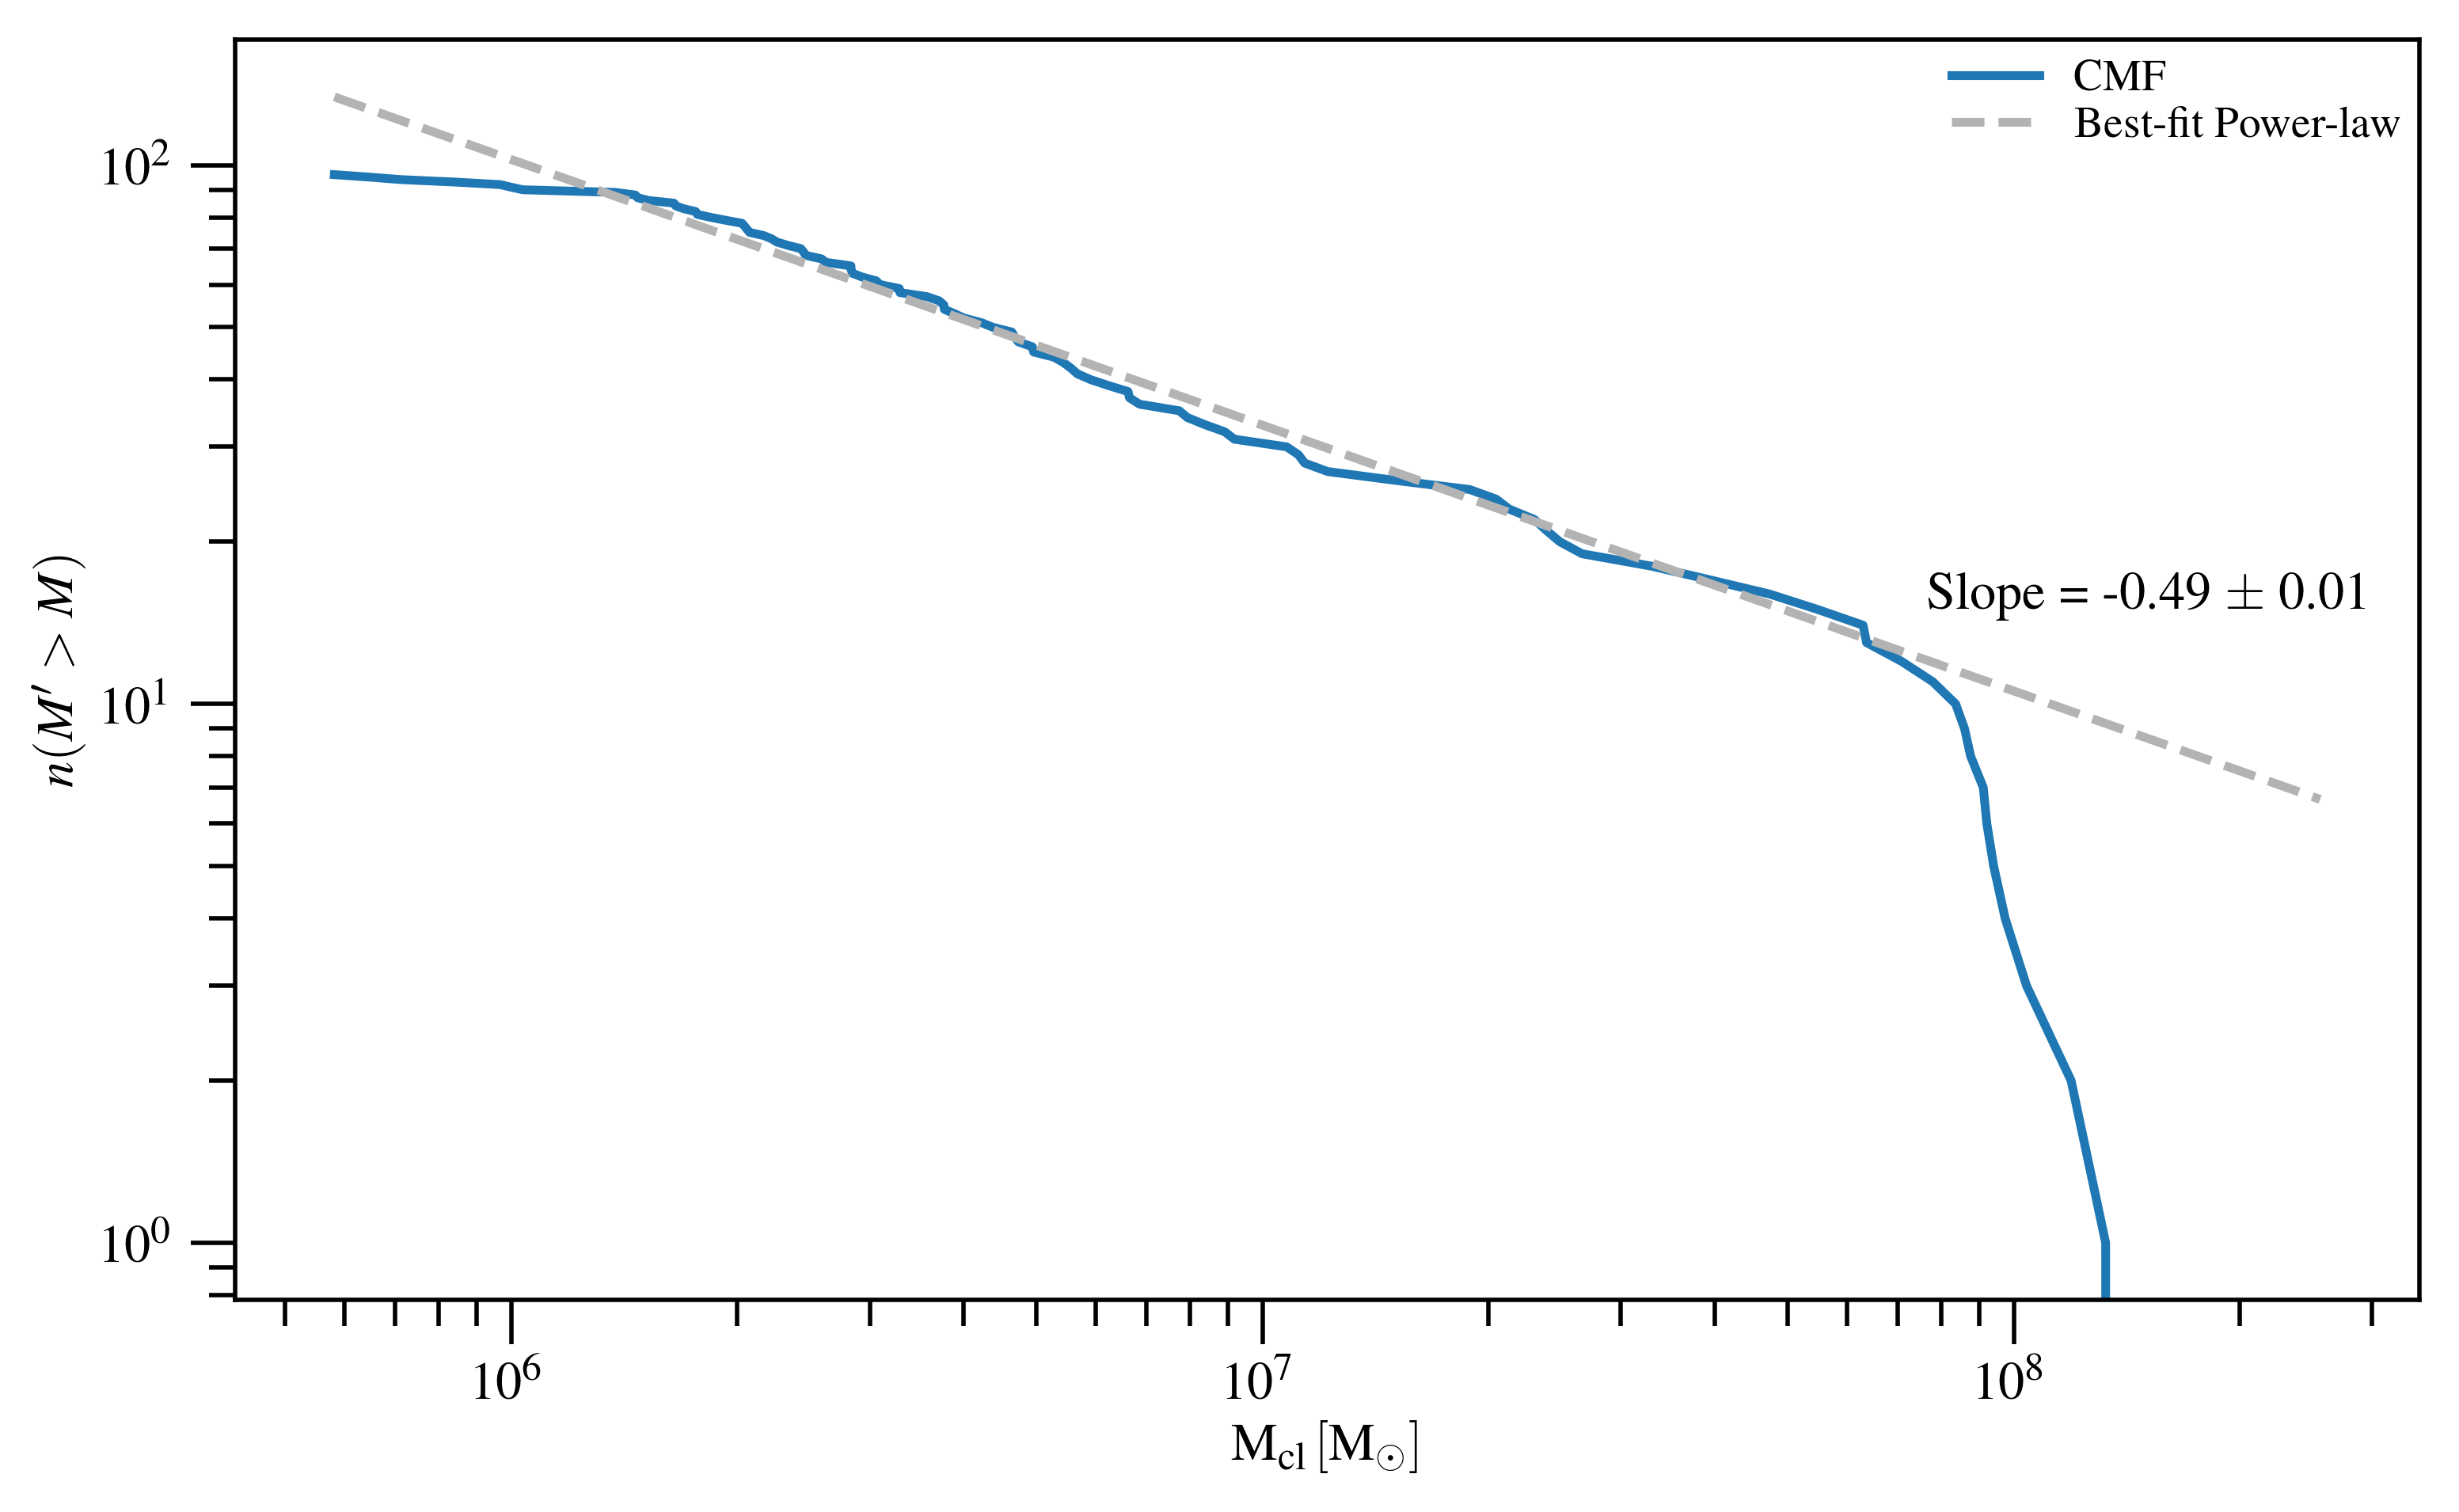
\includegraphics[trim=0 0 0 0, clip, width=0.85\textwidth]{\figpath/CMF_.png}
\caption{
CMF of MCs in \flower and best-fit power law.
\label{fig:cmf}}
\end{figure*}

The range of masses of the MCs identified are consistent with the mass range observed in \z$\sim$2 galaxies in $i$-band light (rest-frame visible),
between $M_{\rm cl}\approx$10$^{7-9}$\,\Msun \citep{Elmegreen07a, Elmegreen09a}.

Noisy due to resolution effect, since we only have one galaxy here. However,
we could improve the ``signal-to-noise'' ratio by including clouds identified from different
snapshots\footnote{This approach is valid unless in some snapshots,
the galaxy experience a violent event, which is relatively rare across the few 100\,Myr studied here.}.
We fit a power-law to the cumulative mass function (CMF), expressed in the form of 
\begin{equation}
n\left(M^\prime > M\right) \propto M_{\rm cl}^\alpha,
\end{equation}
where $n$ is the number of MCs with masses exceeding $M_{\rm cl}$ and $\alpha$ is the power-law index.
The slope varies from $-$0.49\pmm0.01 to $-$1.17\pmm0.06 for MCs identified using the lowest and the
highest $n_{\rm cut}$ adopted in this study.
The uncertainties here are the formal fitting uncertainties.
Regardless of the density threshold adopted, the slope of the CMF of \flower (\Fig{cmf})
is shallower compared to those observed in nearby galaxies (between $-$1.6 and $-$2.5; based on a sample of
$\sim$70 resolved GMCs in M31, M33, IC10 and the Magellanic Clouds; \citealt{Blitz07a}). % between -1.6 to -2.5, mostly -1.7, except for M33, which is -2.5

% interpretation
A higher $\sigma$ and $\Sigma_{\rm gas}$ is related to the higher
pressure. The higher $\Sigma_{\rm gas}$ is also related to more massive clouds being formed.
In M64, there are few clouds with masses $M_{\rm cl}>$10$^7$\,\Msun, such massive molecular
structures are unknown to local group, and are likely the ... from which massive clusters or OB associations are to be formed.
In CMZ, we have seen molecular clouds with high pressures $P/k_B > $10$^7$\,K\,cm$^{-3}$. % also, seen in massive star-forming regions, such as 30 Doradus.

% a bit on caveat
While our result, of particular relevance here is the slope of the CMF, is subject
to the uncertainties in the analysis method and the resolution of our simulation --- i.e., that is
we are likely biased to finding more massive clouds.
High resolution simulations will be useful to shed light on
the evolving dynamical properties of the lower-mass molecular structures in
galaxies at EoR; however, they are more expensive to run.
On the contrary, an advantage of using cosmological zoom-in simulations for this study
is that our computational boxes are not closed, allowing us to examine how
the molecular complexes' properties vary under the influence of gas inflow/outflow.




%--------------------------------------------------------------------------
%                                Discussion
%--------------------------------------------------------------------------
\section{Discussions and Implications}     \label{sec:diss}


\AP{This would be something like \quotes{origin of the cloud and implication of the found properties} if we put there toomre and CMF}

Yet.... at the epoch of reionization.... For instance, to resolve the
\aco line emission in a $L^*$ prototypical galaxy at \z$\sim$6 on xxx\,pc
require .... on-source time even with ALMA.

Connection to observations

The largest molecular structure identified is essentially the main disk of \flower, which is ``broken'' down into smaller
spatial and mass structures that are also denser as we increase $n_{\rm cut}$. In any case,
the MCs we identified are much bigger in size and mass than nearby GMCs, which is consistent with
those observed in \z$\sim$2\,$-$\,4 galaxies with spatially resolved \obs.
The high pressure observed in \flower is also comparable to what has been observed in local ULIRGs; however, the 
molecular clouds in the latter are concentrated within their central regions and have typical sizes of $\sim$70$-$100\,pc and masses on the order of $\sim$10$^9$\,\Msun
\citep{Downes98a, Sakamoto08a}. In our simulation, the high pressure MCs of \flower are 
found throughout the disk. This difference likely stems from the different physical mechanisms giving rise 
to the formation (and thus the nature) of these molecular structures. 
For instance, in local ULIRGs, they are probably form by shock compression or cloud-cloud 
collision after the large amount of gas from the progenitor galaxy merger 
is being funneled toward the central region \citep{Tan00a, Wu18a},  % Tasker09a
whereas in \flower, which is actively accreting gaseous materials 
from the surrounding, they are probably form from constant cold gas accretion onto the entire galaxy (without 
funneling into the center).
This latter mechanism may also be the dominant mode for forming the highly supersonic massive MCs observed 
in gas-rich star-forming galaxies at $z$\ssim2 (see also e.g., \citealt{}).

Looking at correlations between physical parameters such as xx, yy, zz and the CMF
can provide valuable information for developing models of \SF at EoR and
galaxy evolution.


\subsection{Virial Parameter}

\AP{I would move it to the previous section; since it is not easy to condense the toomre analysis for different snapshots in a single plot, I would use the virial parameter analysis to discuss the gravitational instability point on more then on evolutionary state of the galaxy}

We quantify how stable a molecular structure is using the virial parameter, which
describes the balance between pressure support and gravity.

The high $\alpha_{\rm vir}$ suggest that the majority of the MCs identified are not collapsing.
The largest structures are presumably supported by galactic rotation and turbulence from the feedback of
multiple episodes of \SF.
Turbulence in the smaller denser clouds are expected to cascade down over a timescale of $\sim$xxx\,Myr, after which the cloud will collapse
(its substructure likely collapses earlier than this timescale since turbulences would have dissipated).

While it may appear that there is an inconsistency between the high $\alpha_{\rm vir}$
nature of the majority of the molecular gas in \flower and its SFR.
That is, if most of the molecular gas in \flower has high $\alpha_{\rm vir}$, why does it sustain its high SFR of $\sim$100\,\Msun\,yr\pmOne?
This discrepancy can be explained in two ways.
First, our results are limited by the resolution of the simulation, such that, in each MC, there
likely exist multiple smaller-scales molecular structures (e.g., clumps and cores),
as in the classical MC hierarchy. These smaller structures likely no longer supported by large-scale gravitational potential and differential rotation,
and turbulence has dissipated rapidly on these scales to enable collapse \citep{Clark04a}.
Non-axisymmetric perturbations (e.g., arms) to the gravitational potential
can induce orbit crossing, shocks and dissipation in gas, promoting turbulence dissipation.
Note also that \citet{Pettitt18a} report that the virial parameter could be a poor indicator
for the star-forming capacity of the massive (10$^{5-6}$\,\Msun) ``clouds'' in their simulation. They
do not find any significant correlation between $\alpha_{\rm vir}$ and cloud mass
and the star formation efficiency ($M_*/M_{\rm cl}$).


\subsection{CMF and IMF at EoR}

While first stars and galaxies are cooled predominated via H$_2$ lines.
As shown in the $T-n$ phase plot in Fig. 8 of \citealt{Pallottini17b}, metals also play an important role in the cooling of early galaxies.


CMF influences the IMF because .. different cooling properties will lead to different xxx, and thus, Jeans mass/thus determines the final properties of the cloud fragmentation....  For instance, massive protostellar clumps are always supersonic, thus their internal structure are complex. They may form multiple stars.


The minimum clump mass $M_{\rm min}$ is limited by numerical resolution of our simulation. We do not have a resolution study (in hand) and so we cannot quantitatively evaluate this at the moment. The minimum clump mass allowed
by our clump finding algorithm is the mass over 10 cells that exceeds the given threshold density.



%--------------------------------------------------------------------------
%                                Conclusions
%--------------------------------------------------------------------------
\section{Summary and Conclusions}      \label{sec:conclusion}

We study the dynamical properties of molecular complexes in a \z$\sim$6 lyman-break galaxy,
at the end of the epoch of reionization using state-of-the-art cosmological zoom-in simulation
(\ncode{Serra}). We identify molecular cloud complexes in the main galaxy of the
simulated 20\,Mpc h\pmOne box (aka \flower; \citealt{Pallottini17a}) using a method analogues
to the kd-tree idea. We decompose the molecular structures into non-overlapping tiles
% (stored in a kd-tree)
by identifying a set of different density contours at different snapshots.
Using volumetric H$_2$ is essentially the same as identified molecular structures using
different contours in line emission (e.g., CO, CS, NH$_3$)
% and different molecular line tracers trace different MCs on different scales due to their
% different critical densities.
since the line luminosity scales with the molecular gas density.
Our simulations include the effect of feedback from .... .and ....., which are the main source
of non-thermal pressure ejected into the ISM.
We examine the properties of the complexes' at different evolutionary stages and compare
them with nearby and \highz observations. In particular,
the scaling relations between velocity dispersion, complex size, gas mass,
and SFRs.

We find that our results are robust to the various density cuts of choice.
This stems from the
fact that ..... Our choice of density cut is analogues to the inherent problem of limited S/N
in observations.
However, our results are dependent on the numerical resolution of the simulation.

Utilizing high-resolution realistic hydrodynamics simulation with
detailed physics (e.g., feedback and chemical evolution), we
..... , which will become possible to confirm and ... by tracing
the molecular gas emission with future .... such as the Next Generation Very Large Array (ngVLA).
High resolution zoom-in simulations, such as \ncode{Serra}, while inherently limited in galaxy
statistics, provides a way to examine and postulate the morphology and dynamics of
the multi-phase ISM structures of the first galaxies and their satellite galaxies.

Determining the multi-phase ISM properties of early galaxies
is a critical piece to understanding the evolution and
assembly history of galaxies, since they set the pace
for chemical reactions and excitation rates for the coolants in the ISM (and subsequent star formation).
Observations leveraging the combination of spatio-spectral imaging of
multi-band continuum and spectral line emission are crucial for better understanding
the role of \highz galaxy populations
(e.g., LBGs, BzKs, and DSFGs) in
galaxy evolution and the ISM physics behind their intense star formation in the early universe
(if only the ALMA TAC will give us to the time to do so)...


%==============================================================================
%                                Back matters
%==============================================================================
% ACKNOWLEDGEMENTS
%-------------------------------------
\acknowledgements

We thank Jens Kauffmann, Thushara Pillai, and Mark Swinbank for sharing their data.
T.K.D.L. acknowledges support by the NSF through award SOSPA4-009
from the NRAO and support from the Simons Foundation.
A.F. acknowledges support from the ERC Advanced Grant INTERSTELLAR H2020/740120.
This work was initiated as a project for the Kavli Summer Program in Astrophysics (KSPA)
held at the Center for
Computational Astrophysics of the Flatiron Institute in 2018. The program was co-funded by the Kavli
Foundation and the Simons Foundation.
We thank the KSPA Scientific and Local Organizing Committees, and the program founder,
Pascale Garaud for supporting the genesis of this work.
We also thank the New York University CCPP for their hospitality in hosting us, the refugees, after the steam pipe explosion in NYC during the KSPA.


\bibliographystyle{yahapj}
\bibliography{master_cleanup}



\appendix
\section{Schmidt-Kennicutt Relation}
As benchmarking, we check the SK relation of the MCs identified based on their SFR and gas surface densities.
We show in \Fig{sk} the MCs of \flower, identified using different $n_{\rm cut}$ in the ``accreting snapshot'' 
(see \Sec{sfh} for details) compared to those reported in \obs. 

\AP{i m currently a bit confused on how to re-generate pickle files to be used for the plot}
\DL{by running test\_brute.py}

\AP{I would put a figure with the SK-relation for the clumps in a single snapshot for different cuts, along with the observed points and the global \flower point from the data found in \citet{Pallottini17b}}
\DL{to do... after getting points from Pallo, then update plot\_cloud\_prop.py and plotsingleSS.py (uncomment plot\_suff(SK) and only plot snapshot 16)}


\begin{figure*}[htbp]
\centering
\includegraphics[trim=0 0 0 0, clip, width=0.85\textwidth]{\figpath/}
\caption{
SFR and gas surface densities of MCs identified in \flower in \ncode{serra} (xxx symbol) compared to those 
observed in 0$\lesssim$\,\z$\lesssim$2 galaxies (xxx symbol). 
The literature data are compiled from \citealt{Leroy13a, Genzel13a, Sharon13a, Hodge15a}, \citealt{Pallottini17b} and references therein, and Sharon et al. in prep.
\label{fig:sk}}
\end{figure*}




%

%
\end{document}
